\documentclass[
	12pt,				% tamanho da fonte
	oneside,			% para impressão em verso e anverso. Oposto a oneside
	a4paper,			% tamanho do papel. 
	brazil				% o último idioma é o principal do documento]{article}
]{abntex2}

% ---
% Pacotes básicos 
% ---
\usepackage{fontspec}

\usepackage[utf8]{inputenc}		% Codificacao do documento (conversão automática dos acentos)
\usepackage[T1]{fontenc}
\usepackage{indentfirst}		% Indenta o primeiro parágrafo de cada seção.
\usepackage{color}				% Controle das cores
\usepackage{graphicx}			% Inclusão de gráficos
\usepackage{microtype} 			% para melhorias de justificação
\usepackage{multicol}			% multiplas colunas no texto 
\usepackage{booktabs}
\usepackage{tabularx}
\usepackage{natbib, bibentry}
% ---

% ---
% Pacotes de citações
% ---
\usepackage[brazilian]{backref}	 % Paginas com as citações na bibl

\usepackage[dvipsnames,table]{xcolor}
\usepackage[export]{adjustbox}
\usepackage{float}
\usepackage{amsmath}
\DeclareMathOperator{\atantwo}{atan2}
\DeclareMathOperator{\arctantwo}{arctan2}

% --- 
\usepackage{hyperref} % criar hyperlinks
\usepackage[hyphenbreaks]{breakurl}
\usepackage{listings} % utilizado para dar highlight em código
\usepackage[dvipsnames]{xcolor}
\usepackage[export]{adjustbox}
\usepackage[top=3cm, bottom=2cm, left=3cm, right=2cm]{geometry}
\renewcommand{\baselinestretch}{1.5} % espaçamento entre linhas
%\setlength{\parskip}{0.5cm} % espaçamento entre paragrafos
%\setlength{\parindent}{2cm} % recuo do parágrafo
\usepackage{times}
% ---


\lstdefinestyle{customc}{ %custom color para código do arduino
  belowcaptionskip=1\baselineskip,
  backgroundcolor=\color{lightgray},
  breaklines=true,
  frame=single,
  xleftmargin=\parindent,
  language=C,
  showstringspaces=false,
  basicstyle=\footnotesize\ttfamily,
  keywordstyle=\bfseries\color{ForestGreen},
  commentstyle=\itshape\color{darkgray},
  identifierstyle=\color{blue},
  stringstyle=\color{gray},
  breaklines=true,
  morekeywords={bool}
}

% --- 
% CONFIGURAÇÕES DE PACOTES
% --- 

% ---
% Configurações do pacote backref
% Usado sem a opção hyperpageref de backref
%\renewcommand{\backrefpagesname}{Citado na(s) página(s):~}
% Texto padrão antes do número das páginas
%\renewcommand{\backref}{}
% Define os textos da citação
\renewcommand*{\backrefalt}[4]{
	\ifcase #1 %
		Nenhuma citação no texto.%
	\or
		Citado na página #2.%
	\else
		Citado #1 vezes nas páginas #2.%
	\fi}%
% ---

% ---
% Formato da capa de acordo com padrão FSA
\makeatletter

\renewcommand{\folhaderostocontent}{
\begin{center}
    
{\ABNTEXchapterfont\large\imprimirautor}

\vspace*{\fill}\vspace*{\fill}

\begin{center}
\ABNTEXchapterfont\bfseries\Large\imprimirtitulo
\end{center}

\vspace*{\fill}

\abntex@ifnotempty{\imprimirpreambulo}{%
  \hspace{.45\textwidth}
  \begin{minipage}{.5\textwidth}
  \SingleSpacing
  \imprimirpreambulo
  \end{minipage}%
}%

\abntex@ifnotempty{\imprimirpreambulo}{%
  \hspace{.45\textwidth}
  \begin{minipage}{.5\textwidth}
  \SingleSpacing
  Orientador:\\Prof. Dr. Marcos Forte
  \end{minipage}%
  \vspace*{\fill}
}%

\vspace*{\fill}

{\large\imprimirlocal}

\par

{\large\imprimirdata}
\vspace*{1cm}
\end{center}
}
\makeatother
% ---

% ---
% Informações de dados para CAPA e FOLHA DE ROSTO
% ---
\titulo{Sistema de acompanhamento de transporte público para deficientes visuais }
\autor{Arthur Cicuto Pires\\Victor Vieira Paulino}
\local{Santo André}
\data{2017}


\instituicao{%
  Centro Universitário Fundação Santo André -- CUFSA
  \par
  Engenharia de Computação com Ênfase em Software}
  
\tipotrabalho{Conclusão de Curso}
% O preambulo deve conter o tipo do trabalho, o objetivo, 
% o nome da instituição e a área de concentração 
\orientador{Prof. Dr. Marcos Forte}
\preambulo{Trabalho de Conclusão de Curso apresentado à Faculdade de Engenharia “Engenheiro Celso Daniel” do Centro Universitário Fundação Santo André, como exigência parcial para obtenção do grau de Bacharel em Engenharia de Computação.}
% ---

\usepackage[alf]{abntex2cite}	% Citações padrão ABNT
\newcommand{\citecustom}[1]{[\citeauthoronline{#1}, \citeyear{#1}]}
% ---
% Configurações de aparência do PDF final

% alterando o aspecto da cor azul
\definecolor{blue}{RGB}{41,5,195}
\definecolor{bluesky}{RGB}{0,191,255}
\definecolor{red}{RGB}{255,99,71}

% informações do PDF
\makeatletter
\hypersetup{
     	%pagebackref=true,
		pdftitle={\@title}, 
		pdfauthor={\@author},
    	pdfsubject={\imprimirpreambulo},
	    pdfcreator={LaTeX with abnTeX2},
		colorlinks=true,       		% false: boxed links; true: colored links
    	linkcolor=black,          	% color of internal links
    	citecolor=black,        		% color of links to bibliography
    	filecolor=magenta,      		% color of file links
		urlcolor=black,
		bookmarksdepth=4
}
\makeatother
% --- 

% --- 
% Espaçamentos entre linhas e parágrafos 
% --- 

% O tamanho do parágrafo é dado por:
\setlength{\parindent}{1.3cm}

% Controle do espaçamento entre um parágrafo e outro:
\setlength{\parskip}{0.2cm}  % tente também \onelineskip

% ---
% compila o indice
% ---
%\makeindex
% ---

\newcommand*{\BeginNoToc}{%
  \addtocontents{toc}{%
    \edef\protect\SavedTocDepth{\protect\the\protect\value{tocdepth}}%
  }%
  \addtocontents{toc}{%
    \protect\setcounter{tocdepth}{-10}%
  }%
}
\newcommand*{\EndNoToc}{%
  \addtocontents{toc}{%
    \protect\setcounter{tocdepth}{\protect\SavedTocDepth}%
  }%
}



% ----
% Início do documento
% ----

\begin{document}

% Seleciona o idioma do documento (conforme pacotes do babel)
%\selectlanguage{english}
%\selectlanguage{brazil}

% Retira espaço extra obsoleto entre as frases.
\frenchspacing 

% ----------------------------------------------------------
% ELEMENTOS PRÉ-TEXTUAIS
% ----------------------------------------------------------
\pretextual
\begin{figure}[H]
\centering % este comando é usado para centralizar a figura

\includegraphics[width=4.5cm, height=2cm]{images/logo-fsa.jpg}\\
\end{figure}
% ---
% Capa
% ---
\imprimircapa
% ---

% ---
% Folha de rosto
% (o * indica que haverá a ficha bibliográfica)
% ---
\imprimirfolhaderosto

%---

% ----------------------------------------------------------
%Início da folha de aprovação 
% ----------------------------------------------------------
%\begin{folhadeaprovacao} 
%\begin{center} 
%{\ABNTEXchapterfont\large\textsc{\imprimirautor}}
%\\
%\vspace{1cm}
%{\ABNTEXchapterfont\Large\bfseries\imprimirtitulo} 
%\end{center} 
%\vspace{1cm} 
%\hspace{.45\textwidth} 
%\begin{minipage}{.5\textwidth} 
%\imprimirpreambulo 
%\end{minipage} 
%\vspace{1cm} 
%\\Trabalho aprovado. \imprimirlocal, \imprimirdata: 

%Assinaturas 

%\assinatura{\imprimirorientador \\CUFSA} 
%\assinatura{Nome 1\\ CUFSA} 
%\assinatura{Nome 2 \\ CUFSA} 

%\begin{center} 
%\vfill 
%{\large\imprimirlocal} 
%\par 
%{\large\imprimirdata} 
%\end{center} 
%\end{folhadeaprovacao} 
% ----------------------------------------------------------
%Fim da folha de aprovação 
% ----------------------------------------------------------

\begin{agradecimentos} 
Ao nosso orientador Prof. Dr. Marcos Forte, pela paciência e suporte prestado durante o desenvolvimento deste projeto.

Ao Instituto de Cegos Padre Chico, pela hospitalidade demonstrada em nossa visita.

Ao Metractive, pelo incentivo e apoio ao uso de tecnologias.

Ao Raul Bertolo e à Caroline Grava pelo apoio proporcionado.

Às nossas famílias e amigos, pela compreensão e apoio durante esse ano.
\end{agradecimentos} 

% ---
% RESUMOS
% ---

% resumo em português
\setlength{\absparsep}{18pt} % ajusta o espaçamento dos parágrafos do resumo
\begin{resumo}
 
Segundo o IBGE, 3,6\% da população brasileira possui alguma deficiência visual. Deficiência esta, que dificulta a execução de diversas atividades cotidianas, como, por exemplo, a locomoção no perímetro urbano usando transporte público. Com o objetivo de auxiliar a locomoção desses deficientes foi desenvolvido um sistema de escolha de linha e de previsão de chegada de ônibus, visto que o cenário atual não apresenta soluções práticas para esse público-alvo. Para compor o sistema proposto foram desenvolvidos: um aplicativo para smartphone baseados em Android; uma aplicação Web (API); além de módulos de hardware/software para as paradas e para os ônibus. A acessibilidade do aplicativo foi projetada detalhadamente, sendo implementado o feedback auditivo e por vibração, além da detecção automática do ponto onde o deficiente se localiza.  A aplicação gera a lista de linhas de ônibus que passam pelo respectivo ponto, realizando os cálculos de distância e tempo, avisando ao usuário o tempo estimado de espera. O módulo do ônibus envia, em tempo real, a localização atual do ônibus e também avisa ao motorista que há um deficiente visual aguardando no próximo ponto.  Por fim, após a implementação do sistema proposto, incluindo o desenvolvimento dos protótipos dos módulos do ponto e do ônibus, foram realizados testes para verificar se as funcionalidades definidas em projeto foram atendidas adequadamente. 

 \textbf{Palavras-chave}: Acessibilidade, deficientes visuais, smartphone, transporte público, aplicativo mobile.
\end{resumo}

\begin{resumo}[Abstract] 
\begin{otherlanguage*}{english}

According to the IBGE, 3,6\% of Brazil's population have some kind of visual impairment. This deficiency, hinder the execution of various everyday activities, like, for example, the usage of public transportation in the urban perimeter. With the objective to help the visual impaired to move around, it was developed a system to choose a bus line and give the bus arrival prediction, as the actual scene doesn't show practical solutions for the target audience. To compose the suggested system, it was developed: an application for Android based smartphones; a Web application (API); and hardware/software modules for the bus stops and the buses. The application accessibility was designed in detail, being implemented
a feedback by audio and by vibration, besides the automatic detection of the bus stop where the visual impaired is. The application generates a list of the bus lines that go through that bus stop, doing the distance and arrival forecast calculations, notifying the user the estimated waiting time. The bus module sends, in real time, the bus actual location and warns the user that there is a visual impaired waiting in the next bus stop. Lastly, after the implementation of the system proposed, including the bus and bus stop modules prototypes development, were made some tests to see if the defined functionalities answer accordingly.

\vspace{\onelineskip} 
\noindent \textbf{Keywords}: Acessibility, visually impaired, smartphone, public transportation, mobile application. 
\end{otherlanguage*} 
\end{resumo} 


\listoffigures*\thispagestyle{empty} \newpage

\BeginNoToc
% ---
% inserir o sumario
% ---
\tableofcontents*
% ---
% ---
\EndNoToc

\newpage

% ----------------------------------------------------------
% ELEMENTOS TEXTUAIS
% ----------------------------------------------------------
\textual

\chapter{Introdução}

Segundo o Censo Demográfico de 2010, feito pelo \citecustom{ibge} (Instituto Brasileiro de Geografia e Estatística), no Brasil, existe mais de 6,5 milhões de pessoas com alguma deficiência visual, representando cerca de 3,6\% da população brasileira. Dentre essas pessoas, pouco mais de 500 mil pessoas não conseguem de modo algum enxergar e 6 milhões tem grande dificuldade.

A Fundação Dorina, \citecustom{Dorina2017}, descreve os níveis de deficiência visual da seguinte forma:

\begin{citacao}
A deficiência visual é definida como a perda total ou parcial, congênita ou adquirida, da visão. O nível de acuidade visual pode variar, o que determina dois grupos de deficiência:

Cegueira: há perda total da visão ou pouquíssima capacidade de enxergar, o que leva a pessoa a necessitar do Sistema Braille como meio de leitura e escrita.

Baixa visão ou visão subnormal: caracteriza-se pelo comprometimento do funcionamento visual dos olhos, mesmo após tratamento ou correção. As pessoas com baixa visão podem ler textos impressos ampliados ou com uso de recursos óticos especiais.
\end{citacao}

Como sugere \citecustom{bersch2013}, a tecnologia assistiva tem como objetivo dar maior independência para pessoas com alguma deficiência, aumentando a qualidade de vida através da realização de tarefas desejadas que antes tinham um grau de dificuldade ou eram impossibilitadas de fazer.

O desenvolvimento de recursos e outros elementos de Tecnologia Assistiva tem propiciado a valorização, integração e inclusão da pessoa com deficiência, promovendo seus direitos humanos. Por essa razão, o tema tem assumido um espaço importante nas ações desenvolvidas pela Secretaria Nacional de Promoção dos Direitos da Pessoa com Deficiência e demais órgãos federais, como o Ministério da Saúde, Ministério da Educação e Ministério de Ciência e Tecnologia. \citecustom{PortalSaude2014}

	Dentre os elementos da tecnologia assistiva pode-se utilizar smartphones, que tem se tornado cada vez mais presentes na vida das pessoas. Uma pesquisa realizada pelo FGV-SP em 2016, \citecustom{Meirelles2016}, demonstrou que o número de aparelhos chegou a 168 milhões só no Brasil. Com sua facilidade de acesso, surgem inúmeras soluções que resolvem problemas do dia-a-dia dos usuários.

	Dentre essas soluções, aplicações para smartphones que ajudam na mobilidade são cada vez mais comuns. Os aplicativos CittaMobi, \citecustom{Vieira2015}, e Moovit, \citecustom{Gomes2015}, vieram para mostrar que a tecnologia embarcada nos aparelhos podem ajudar a prever quanto tempo falta para o ônibus chegar em um ponto de parada, em tempo real. Eles capturam a geolocalização do usuário para saber qual ponto de ônibus eles estão próximos, possibilitando o usuário dizer de forma mais rápida qual seu ponto. Informando ao aplicativo qual seu ponto, eles podem selecionar um ônibus que passa no ponto selecionado, para saber quanto tempo resta para o veículo chegar.

Isso ajuda os usuários a se programar melhor, possibilitando a pessoa sair em um horário mais oportuno ou deixando ela mais tranquila sabendo que em breve seu ônibus chegará.

\section{Descrição Geral}

A fim de conhecer melhor sobre as dificuldades que os deficientes visuais encontram para se locomover pelo perímetro urbano utilizando o transporte público, foi realizada uma visita técnica ao Instituto de Cegos Padre Chico, (http://www.padrechico.org.br/). Durante a visita, notamos que os principais pontos levantados por eles foram o medo de ficar com o smartphone em mãos e a vergonha de ter de parar todos os ônibus para saber qual a linha que o veículo atende.

Este trabalho visa facilitar a vida de deficientes visuais que utilizam ônibus como meio de transporte. O aplicativo proposto irá possibilitar ao deficiente visual saber quanto tempo falta para seu ônibus chegar, enquanto o sistema se encarrega de avisar o motorista do ônibus qual o próximo ponto onde terá um deficiente visual esperando por aquele ônibus.

Sistemas operacionais de smartphone, como Android e iOS, possuem ferramentas nativas que adaptam o uso de aplicativos para pessoas com deficiências, possibilitando a utilização do aparelho sem grandes dificuldades, mas, nem sempre, criam boas experiências de uso. 

O Android possui a ferramenta Talkback \citecustom{talkback}, para auxiliar no uso de qualquer aplicativo. Ao desenvolver uma solução para o sistema, é possível colocar tags específicas em cada elemento da tela da sua aplicação. Isso possibilita ao Talkback ler a tela com maiores detalhes para o deficiente visual ou utilizar a função de áudio dele para fazer áudio descrições mais detalhadas sobre o significado de uma tela.

Fazer aplicativos que funcionem em conjunto com essas tecnologias voltadas a deficientes, não é um trabalho difícil, mas criar boas experiências de uso que facilitem a vida de deficientes visuais é uma grande tarefa a ser cumprida.

Por isso é necessário adicionar outras tecnologias que facilitem o uso do app, neste caso, os \textit{Beacons}. \textit{Beacon} é um dispositivo que utiliza Bluetooth 4.0 (que tem baixo consumo de energia). Se existe um smartphone próximo a um \textit{Beacon}, o aplicativo pode informar sua localização com maior precisão que um GPS. \citecustom{beacon}.

Dessa forma quando um deficiente visual chegar no ponto, ele abre o aplicativo e, com uso do \textit{Beacon} instalado no ponto, se detecta automaticamente em qual ponto o deficiente visual está. Sabendo isso, o app lista quais ônibus passam ali. Após o deficiente visual escolher um dos ônibus, o aplicativo vai notificar em intervalos pré-definidos quanto tempo falta para o ônibus chegar, em contrapartida o sistema irá alertar o motorista quando ele estiver próximo ao ponto em que existe um deficiente visual esperando por ele.

\section{Restrições de projeto}

\begin{itemize}
\item O smartphone deve ter o sistema operacional Android 4.1 (API Level 16) ou posterior instalado;
\item O smartphone deve possuir Bluetooth 4.0 LE ou superior;
\item O smartphone deve estar com a função Talkback ativada;
\item O ônibus deve prover sinal de rede Wi-Fi para que o módulo do ônibus possa se comunicar.
\end{itemize}

\chapter{Tecnologias Utilizadas}

Para o desenvolvimento do projeto, foi elaborado um sistema dividido em quatro subsistemas, sendo eles o módulo do ônibus, o \textit{beacon}, o \textit{Web Service} e o aplicativo. Os métodos de comunicação e as tecnologias empregadas nelas estão ilustrados na Figura \ref{tecnologias}. 

\begin{figure}[H]
\centering
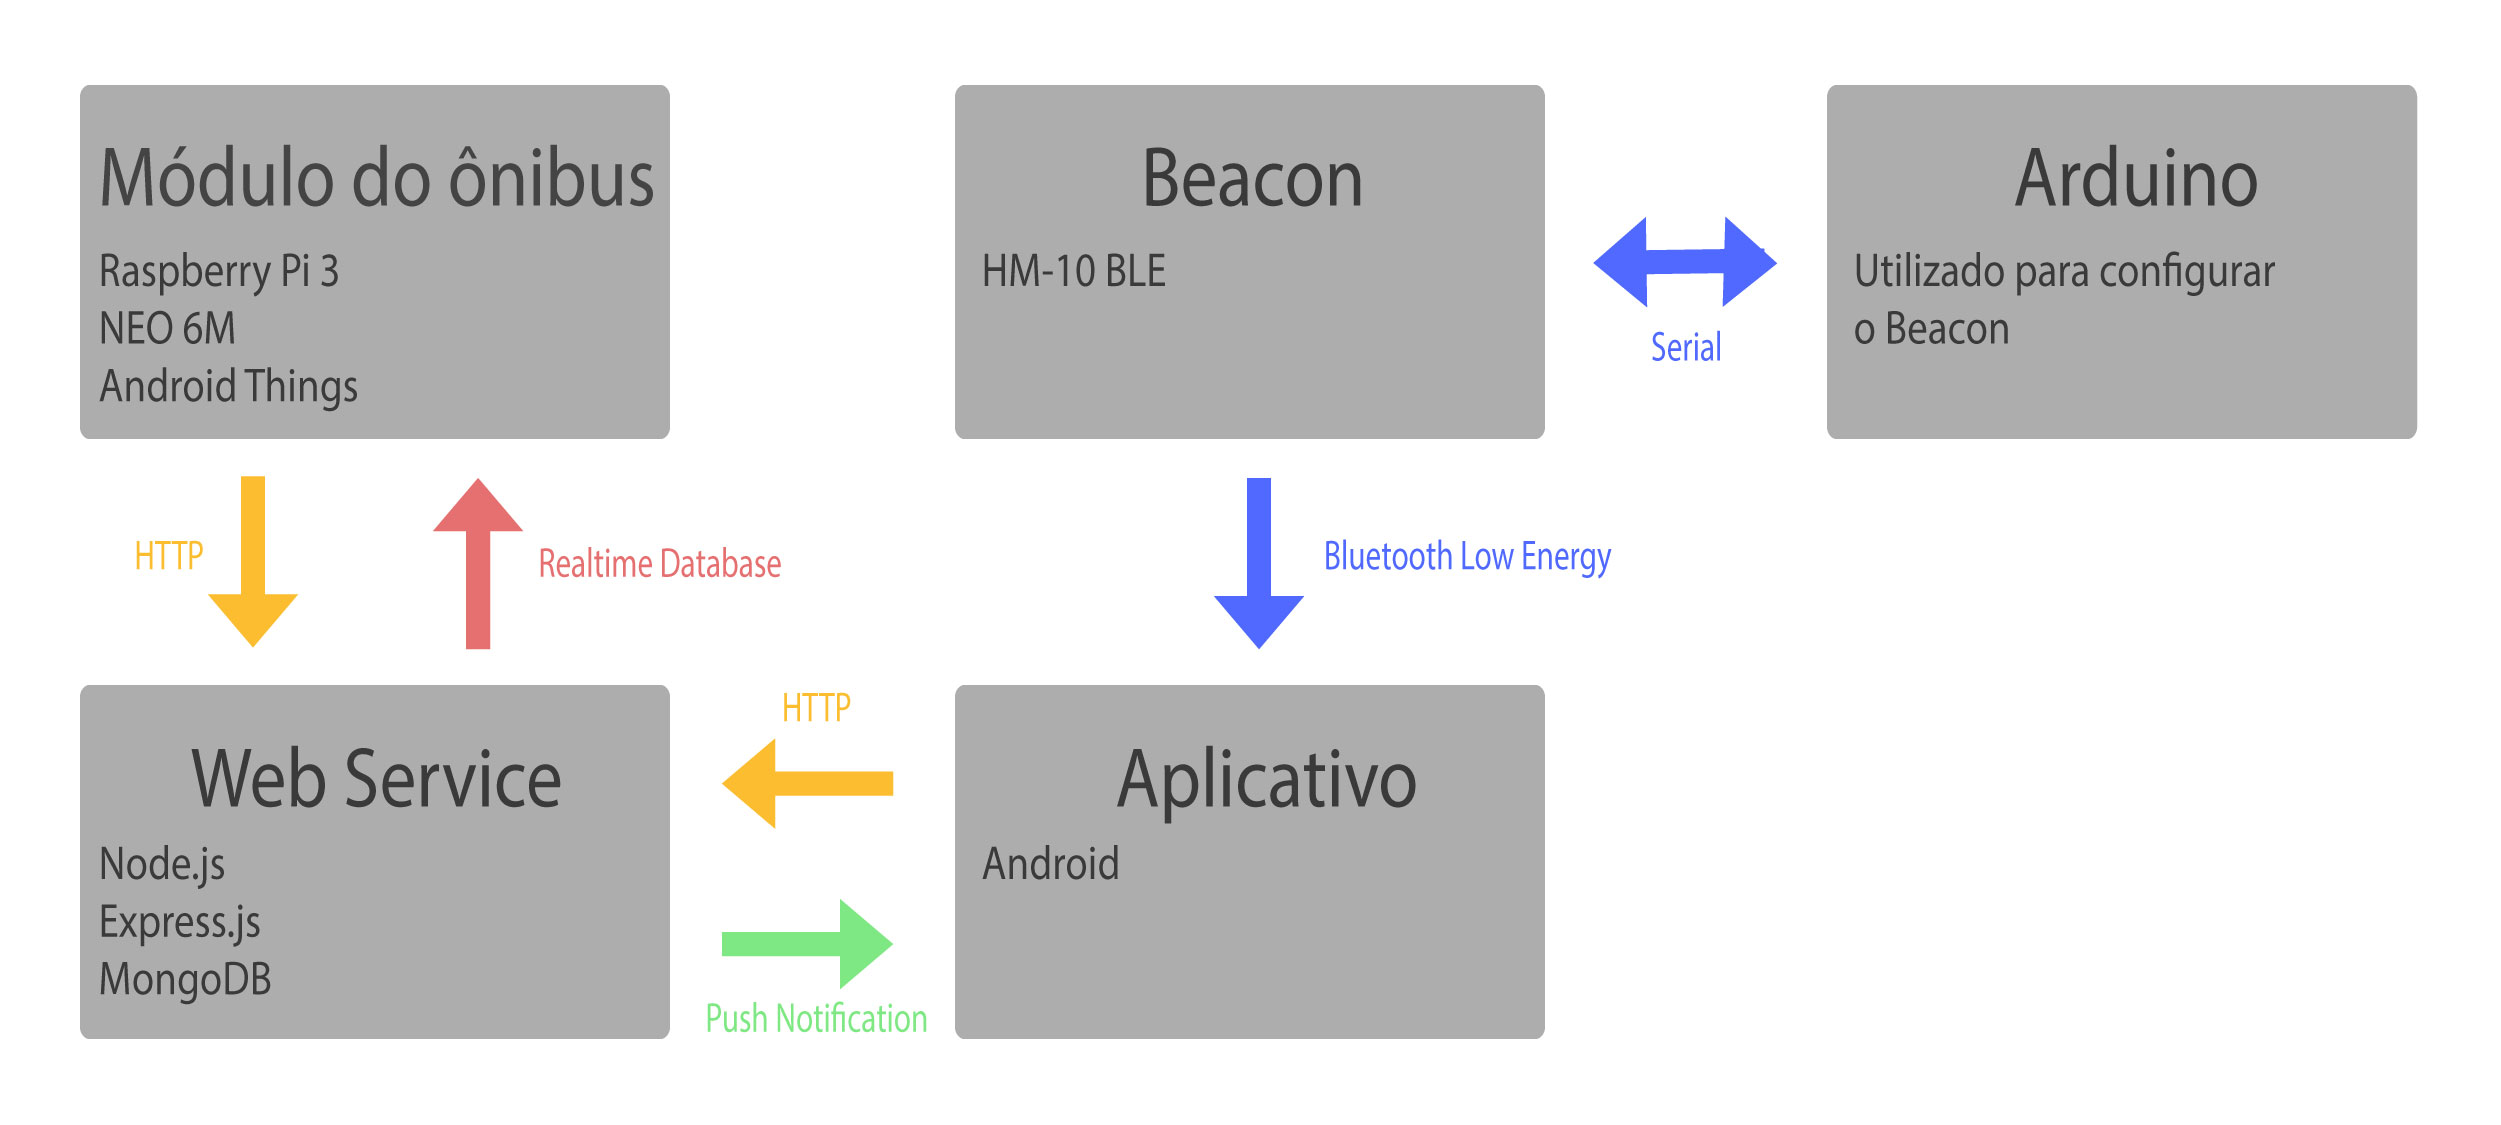
\includegraphics[width=10cm, center]{images/tech}
\caption{Tecnologias utilizadas.}
\label{tecnologias}
\end{figure}

\section{Comunicação}

\subsection{HTTP}

O Protocolo de transferência de hipertexto (do inglês \textit{Hypertext Transfer Protocol}), é um protocolo para tráfego de informações pela internet entre cliente e servidor. Sempre que o cliente deseja transmitir algo para o servidor, é enviada uma requisição \textit{HTTP} contendo nela um cabeçalho, com informações sobre a requisição, e o corpo, contendo uma mensagem a ser entregue. Uma requisição \textit{HTTP} pode ser do tipo GET, POST, PUT, DELETE, HEAD, TRACE, OPTIONS, ou CONNECT, e cada tipo defiine uma determinada ação solicitada pelo cliente ao servidor.
O cabeçalho do protocolo contém o campo \textit{Content-Type} com o tipo de \textit{MIME} contido no corpo da requisição. 

O tipo MIME (\textit{Multipurpose Internet Mail Extensions} - Extensões de correio de Internet multifunções) é um padrão proposto pelos laboratórios \textit{Bell Communications}, em 1991, para aumentar a possibilidade de inserir documentos (imagens, sons, texto, etc.) em uma mensagem. Desde então, o tipo MIME é usado para formatar tanto documentos anexos em uma mensagem quanto os transferidos pelo protocolo HTTP. \citecustom{CCM2017}

\subsection{Push Notification}

Como explica \citecustom{Finzi2016}
 \textit{Push Notification} é um serviço de entrega de mensagens, parecido com \textit{SMS} (\textit{Shot Message Service}), que utiliza a internet para isso. Um caso comum do uso de \textit{push notifications} é quando existe a necessidade de notificar um ou mais usuários de um aplicativo sobre algo, não sendo necessário que a aplicação esteja aberta. Alguns serviços são especializados na entrega de mensagens desse tipo, como o \textit{Firebase Cloud Messaging}, que provê um \textit{SDK} para que o desenvolvedor implemente o serviço de recebimento destas mensagens na sua aplicação para quando for preciso enviar uma mensagem, faça apenas requisições \textit{HTTP} para o serviço e ele se encarregue de entregar a mensagem para os dispositivos disponíveis.

\subsection{Beacons}

O \textit{Beacon} é um pequeno dispositivo que utiliza uma tecnologia chamada \textit{Bluetooth Low Energy} (BLE), que emite um sinal intermitente de ondas de rádio que consegue localizar seu smartphone em um determinado raio de cobertura deste sinal. \citecustom{CarneiroMaio}. 
A grande novidade desses aparelhos, além do custo acessível, é que eles podem ser instalados em paredes, produtos ou vitrines, permitindo a comunicação entre empresa e público por meio da localização e sem a necessidade de acesso à internet, já que utiliza o \textit{bluetooth} do \textit{smartphone} para enviar as mensagens \citecustom{Saes2014}.
Como explica \citecustom{CarneiroOutubro}, \textit{iBeacon} é um protocolo de comunicação para dispositivos \textit{Beacons}, lançado pela \textit{Apple} em 2013. 

De acordo com \citecustom{CarneiroOutubro} as informações do protocolo são formadas da seguinte forma:

\begin{enumerate}

\item Identificador Único Universal (do inglês \textit{Universal Unique Identifier} ou UUID): É a sequência que identifica cada dispositivo.
\item Major: Utilizado para criar grupos de \textit{Beacons}. Assim é possível fazer um filtro com todos dispositivos do mesmo grupo.
\item Minor: Utilizado para criar sub grupos, possibilitando o filtro dentro de grupos (\textit{Major)}.
\item Frequência de Transmissão: Intervalo que o sinal é transmitido.
Poder da transmissão: Alcance máximo do sinal.

\end{enumerate}

\subsection{Realtime Database}

O \textit{Firebase Realtime Database} é um banco de dados hospedado na nuvem. Os dados são armazenados no formato JSON e sincronizados em tempo real com todos os clientes conectados.
Em vez de solicitações HTTP típicas, o \textit{Firebase Realtime Database} usa a sincronização de dados. Sempre que os dados são alterados, todos os dispositivos conectados recebem essa atualização em milissegundos. \citecustom{Firebase}


\section{Hardware}

\subsection{Raspberry Pi 3}

\begin{figure}[H]
\centering
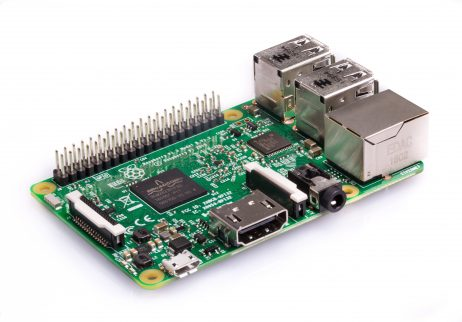
\includegraphics[width=10cm, center]{images/raspberry-pi}
\caption{Raspberry Pi 3}
\fonte{\citeauthor{raspimage}}
\label{Rotulo}
\end{figure}

Segundo Upton \citecustom{Upton2017}, "A \textit{Raspberry Pi} é uma máquina completa, com considerável poder de processamento, em uma placa de circuito impresso menor do que um cartão de crédito. Com ela você pode ter resultados impressionantes.". Esta pequena placa permite ter um computador em um pequeno espaço, contando com conectividades como \textit{Bluetooth} e \textit{WiFi}, é uma excelente opção para projetos que necessitam de mais poder de processamento em um pequeno espaço. 

A \textit{Fundação Raspberry Pi}, responsável pelo seu desenvolvimento, também mantém o foco da placa no meio educacional, apresentando uma plataforma acessível para que cada vez mais pessoas se interessem por desenvolvimento de softwares.

Especificações:

\begin{itemize}
\item Quad Core 1.2GHz Broadcom BCM2837 64bit CPU
\item 1GB RAM
\item BCM43438 \textit{wireless} LAN e \textit{Bluetooth Low Energy} (BLE)
\item 40-pin \textit{extended} GPIO
\item 4 USB 2 ports
\item 4 \textit{Pole stereo output} e \textit{composite video port}
\item Full size HDMI
\item CSI \textit{camera port} para conectar uma câmera \textit{Raspberry Pi}
\item DSI \textit{display port} para conectar um display \textit{touchscreen Raspberry Pi}
\item Micro SD \textit{port} para carregar o sistema operacional e armazenar dados
\end{itemize}


\subsection{HM-10}

\begin{figure}[H]
\centering
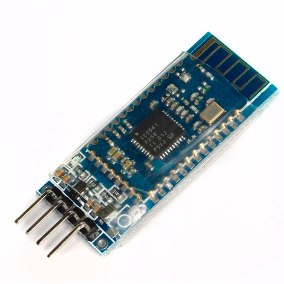
\includegraphics[width=5cm, center]{images/hm-10}
\caption{Módulo Bluetooth HM-10}
\fonte{\citeauthor{hm10image}}
\label{Rotulo}
\end{figure}

A empresa \textit{Jinan Huamao} é responsável pelo desenvolvimento do HM-10 (http://www.jnhuamao.cn/bluetooth.asp), um pequeno módulo \textit{Bluetooth} 4.0 BLE baseado no chip CC2540 que trabalha com alimentação de 3.3V. Com ele é possível realizar comunicações utilizando o protocolo \textit{Bluetooth}.

\subsection{Arduino Uno}

\begin{figure}[H]
\centering
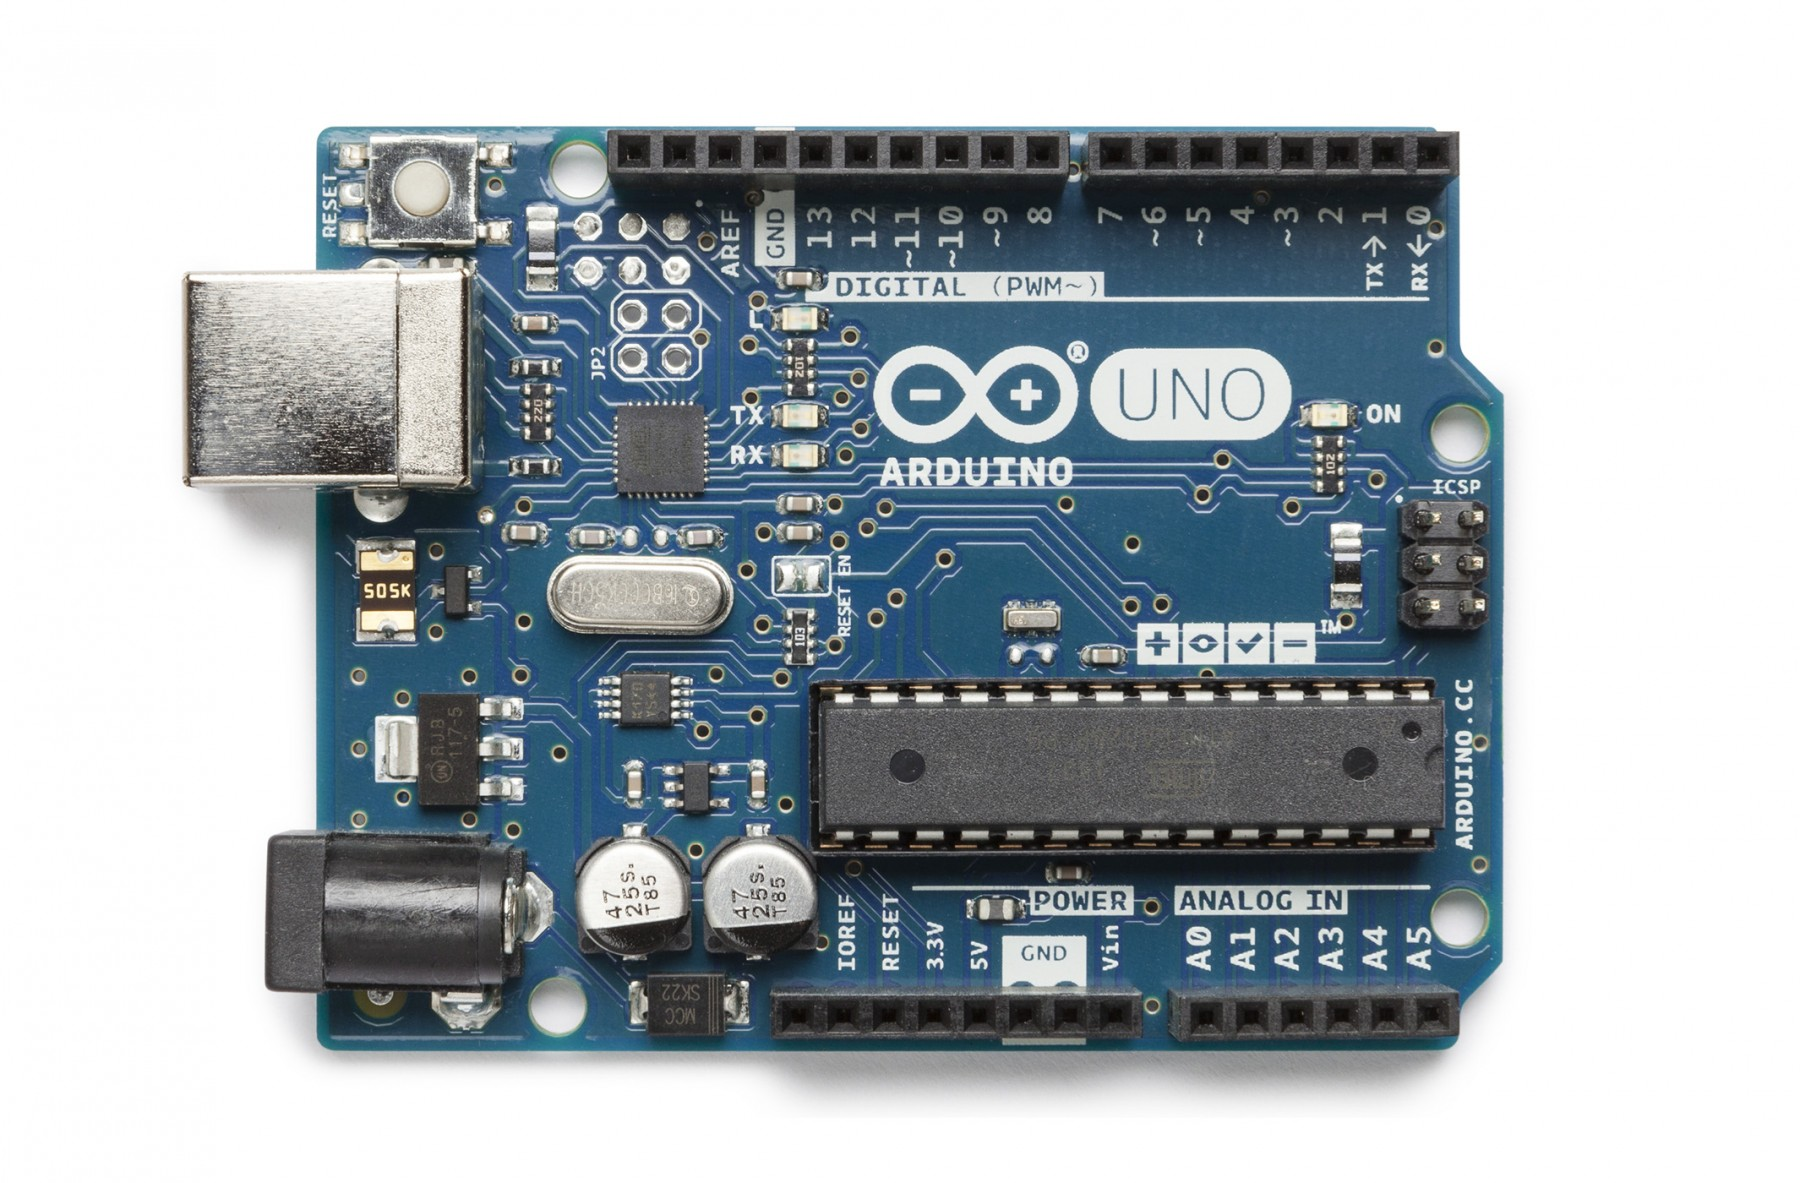
\includegraphics[width=7cm, center]{images/arduino}
\caption{Arduino Uno}
\fonte{\citeauthor{arduinounoimage}}
\label{Rotulo}
\end{figure}

\textit{Arduino} é uma plataforma de prototipagem desenvolvida em 2005, na Itália. Conectando a placa via USB em um computador, é possível programar o microcontrolador Atmel que ela possui, tendo a possibilidade de controlar dispositivos externos por meio de suas portas \textit{GPIO (General Purpose Input/Output)}.

O \textit{Arduino} pode ser utilizado para desenvolver objetos interativos independentes, ou pode ser conectado a um computador, a uma rede, ou até mesmo à Internet para recuperar e enviar dados do \textit{Arduino} e atuar sobre eles. \citecustom{mcroberts2011}

\newpage

\subsection{NEO 6M}

\begin{figure}[H]
\centering
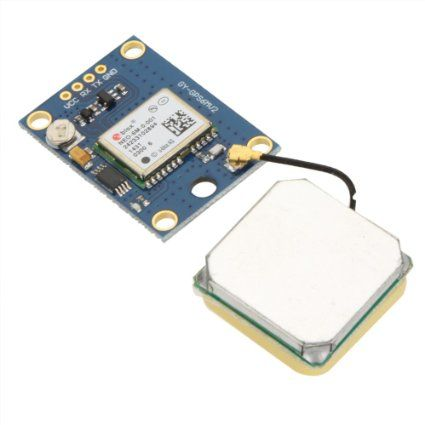
\includegraphics[width=5cm, center]{images/neo-6m}
\caption{Módulo NEO u-blox 6 GPS}
\fonte{\citeauthor{neo6mimage}}
\label{Rotulo}
\end{figure}

O NEO U-BLOX 6 é um módulo que permite obter a geolocalização por meio do \textit{GPS (Global Position System)}. De acordo com \citecustom{sousa2017extraccao} a obtenção da localização no globo é dada pela trilateração dos dados recebidos por pelo menos quatro satélites, onde cada um envia um sinal de sincronismo e em seguida sua posição. 

Para obter os dados do módulo, realiza-se uma comunicação com protocolo UART (Universal Asynchronous Receiver/Transmitter). Tais informações obtidas seguem a especificação NMEA 0183 da (\textit{National Marine Eletronic Association}). No trecho abaixo, \citecustom{sousa2017extraccao}, fala do protocolo no Android:

\begin{citacao}
O protocolo NMEA é o mecanismo de comunicação padrão entre os receptores GPS e os drivers
dos dispositivos receptores na arquitetura Android. Desta forma, os programas que fornecem
soluções de posicionamento precisam decodificar as mensagens NMEA. A ideia do protocolo,
no que diz respeito a coordenadas de posicionamento, consiste em enviar uma linha de dados,
codificada em ASCII, que pode conter informações de posição, velocidade, tempo, dentre
outros elementos processados pelo receptor GPS. 
\end{citacao}

\newpage

\section{Software}

\subsection{Sistemas Operacionais}

\subsubsection{Android}

Existem vários sistemas operacionais voltados para dispositivos móveis, sendo Android o mais popular. O sistema foi desenvolvido pela empresa Android Inc, posteriormente adquirida pela Google Inc. Foi lançado em 2008 e conta com o apoio da \textit{Open Handset Alliance} (um conjunto de empresas que atuam juntas para o melhoramento dos padrões da telefonia e também do desenvolvimento do sistema Android). 

Tal sistema é muito acessível e popular. Está disponível para uma enorme variedade de dispositivos. O Android tem como base o sistema operacional Linux, conhecido por ser um sistema flexível, adaptável a várias arquiteturas de processador, seguro e eficiente. Um dos grandes diferenciais do Android e que contribui para sua popularidade, é o fato de que o sistema é compatível com vários hardwares e pode estar disponível em \textit{smartphones} de diversos fabricantes. \citecustom{Android}

Segundo uma pesquisa feita pela IDC (\textit{International Data Corporation}) no primeiro quadrimestre de 2017, \citecustom{idc}, o Android se mostra um sistema consolidado no mercado, tendo participação de 85\% do mercado. O gráfico da Figura \ref{idc} mostra que desde 2014 é o sistema operacional mais utilizado em dispositivos móveis.

\begin{figure}[H]
\centering
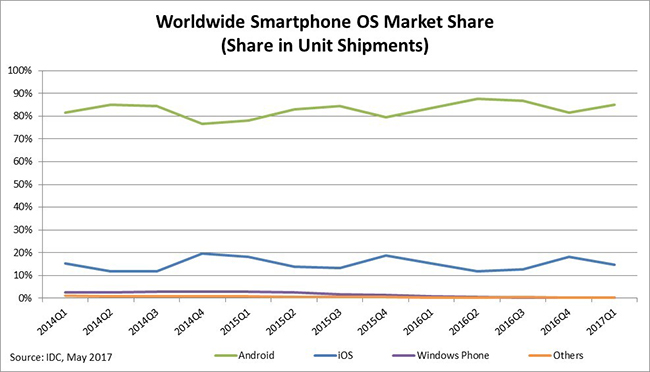
\includegraphics[width=11cm, center]{images/smartphone-share-market.jpg}
\caption{Pesquisa realizada pela IDC}
\fonte{\citeauthor{idc}}
\label{idc}
\end{figure}

\subsubsection{Android Things}

O Android Things foi criado voltado ao mercado \textit{IoT (Internet of Things)} e a partir da versão do Android para \textit{smartphones}, o que possibilitou o suporte a maioria das APIs disponíveis. Utilizando a mesma \textit{IDE} para desenvolvimento, qualquer desenvolvedor Android pode desenvolver soluções \textit{IoT} com os conhecimentos que já possui.
\citecustom{androidthings}

\begin{citacao}
\textit{A comprehensive way to build IoT products with the power of Android, one of the world's most supported operating systems. Now any Android developer can quickly build a smart device using Android APIs and Google services, while staying highly secure with updates direct from Google.} \citecustom{Piekarski2016}
\end{citacao}

Atualmente o sistema tem suporte para rodar nas seguintes plataformas:

\begin{itemize}
\item NXP Pico i.MX7D
\item NXP Pico i.MX6UL
\item NXP Argon i.MX6UL
\item NXP SprIoT i.MX6UL
\item Raspberry Pi 3
\end{itemize}

\textbf{Arquitetura utilizada}

\begin{figure}[H]
\centering
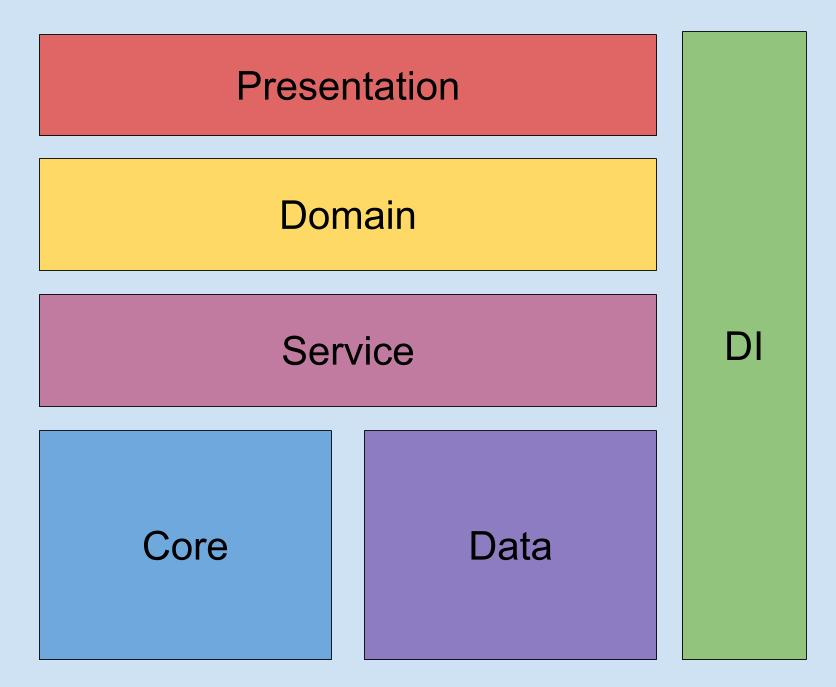
\includegraphics[width=10cm, center]{images/brick_diagram_beacon}
\caption{Diagrama de blocos do aplicativo móvel.}
\label{Rotulo}
\end{figure}

Para desenvolvimento das aplicações que rodam nos sistemas operacionais Android, foi adotado o padrão \textit{Clean Architecture}. Este padrão foi proposto por Robert Ceil Martin (conhecido como Uncle Bob) em \citecustom{martin2012clean}, e foca no domínio da aplicação, fazendo \textit{frameworks} e \textit{drivers} serem detalhes de implementação. Seguindo seus princípios, a estrutura de camadas ficou da seguinte forma:

\begin{description}

\item[Core] Não contém nenhuma lógica de negócio. Esta camada provê informações que são comuns para toda a aplicação, como informações estáticas e algumas classes e interfaces bases.

\item[Data] Responsável por prover dados para toda aplicação. Ela adota o Padrão de Arquitetura \textit{Repository}, tendo uma interface de acesso aos dados. Uma grande vantagem em utilizar essa camada com esse padrão de arquitetura, é o respeito a responsabilidade única, um dos princípios do \textit{SOLID}, \citecustom{solid}. Ela encapsula toda lógica de busca de dados, assim, caso uma classe precise de algum dado específico, ela solicita através da interface de comunicação e, a classe que implementa a interface, cuida de toda lógica de busca de dado, seja um dado armazenado localmente, em \textit{cache} ou em um servidor remoto. Tudo fica transparente para a classe que solicitou o dado.

\item[Service] Provê serviços para qualquer camada. No caso do aplicativo para \textit{smartphone}, a implementação do serviço de voz fica implementada neste pacote. Esta camada não existe no \textit{Android Things}, por não possuir serviços característicos da mesma. 

\item[Domain] Esta camada encapsula todas as regras de negócios da aplicação. Toda vez que é necessário realizar processamentos em dados para satisfazer funcionalidades, são feitos por esta camada.

\item[Presentation] Responsável por toda interface gráfica. Toda lógica de criação de telas e interceptação de interações do usuário com o aplicativo é feito aqui. Quando é necessário procurar dados para exibir ao usuário, são feitas solicitações deles para a camada \textit{Domain} ou \textit{Data} para que seja possível exibir os dados.

\item[DI] Esta camada utiliza o padrão de arquitetura Injeção de Dependências. Esta camada provê todas as dependências, fazendo a implementação mais limpa nas outras classes, já que não precisam saber como instânciar uma classe.
 
\end{description}

\subsubsection{Linguagem de Programação}

Segundo \citecustom{Avram2017}, a Google suportava as linguagens de programação Java e C++ para desenvolvimento de aplicativos Android. Em 2017, foi acrescentado suporte a linguagem Kotlin, por "ser concisa, expressiva e projetada para ser \textit{type-safe} e \textit{null safe}".
Para este trabalho, dentre as três linguagens disponíveis, foi escolhido o Kotlin por demonstrar ser uma linguagem de sintaxe mais simplificada e trabalhar bem, caso necessário, com Java, como cita \citecustom{Kewerson2017}: "Como consequência das boas decisões dos designers da linguagem, temos uma linguagem concisa com a possibilidade de interoperar código Kotlin com Java e Java com Kotlin".

\subsection{Backend}

\subsubsection{Linguagem}

Para o desenvolvimento do \textit{Web Service} foi escolhido um conjunto de tecnologias \textit{server-side} baseadas em JavaScript.

\subsubsubsection{JavaScript}

JavaScript é uma linguagem de programação \textit{client-side}, utilizada para manipular os comportamentos de uma página, controlando o HTML e o CSS. Outra característica é o fato de ser uma linguagem orientada à eventos.

Para explicar melhor o que são eventos, é importante citar que uma página HTML utiliza tags para representar seus elementos, podendo conter menus, botões e formulários, entre outros, em seu corpo. Cada elemento possui alguns atributos, sendo alguns desses chamados atributos de eventos, como por exemplo o \textit{onClick} que realiza alguma função caso o elemento referente seja clicado pelo usuário.

Para especificar as ações que devem ser tomadas quando um evento é acionado, pode-se utilizar o JavaScript. Com o decorrer do tempo, foram desenvolvidas algumas modificações na linguagem JavaScript para possibilitar a utilização do mesmo no \textit{server-side}, possibilitando o desenvolvimento de um \textit{Web Service}. 

Foram escolhidas, como ferramentas, o MongoDB, o Node.js e o Express.js, utilizando o \citecustom{Almeida2016} como referência teórica e prática para conhecer essas tecnologias.

\subsubsection{MongoDB}

É um banco de dados não relacional com uma escalabilidade muito boa. Ele utiliza conceitos de \textit{collections} e \textit{documents} em sua construção. 

As \textit{collections} são equivalentes aos bancos de um ambiente que utiliza o SQL. Já os \textit{documents}, se equivalem aos registros de cada banco. Os dados são guardados em arquivos similares aos de formato JSON (\textit{JavaScript Object Notation}).

Outro item importante sobre o MongoDB é o fato de ser \textit{schemaless}, tornando-o bem flexível em relação a inclusão de dados diferentes em uma mesma \textit{collection}, fazendo com que a validação de dados fique nas mãos dos desenvolvedores.

Apesar de \textit{schemaless}, é possível criar \textit{schemas} para auxiliar no desenvolvimento. Ao utilizar o mongoose, ferramenta desenvolvida em cima do MongoDB para trabalhar nele como se estivesse utilizando um banco relacional, é possível definir de antemão, quais os atributos que devem existir em cada \textit{collection} necessária para a aplicação.


\subsubsection{Node.js}

Plataforma principal para o funcionamento da aplicação, construída sobre o motor Javascript V8 do Google Chrome.
O Node.js foi desenvolvido para construir aplicações \textit{web} escaláveis de forma assíncrona, cuidando de várias conexões de maneira concorrente. Ele consegue isso através da utilização de \textit{callbacks}. \citecustom{Node2016}

Sempre que ocorre um evento, é disparado um \textit{callback} que dirá o que deve ser realizado pela aplicação. Esse processo é feito para todas as funções presentes na aplicação e sempre que houver um evento sendo disparado.

Como no lado do servidor, não existe uma interface gráfica a ser visualizada, os eventos nesse caso são dados de I/O, como algum parâmetro usado em uma busca no banco de dados, a resposta para aquele parâmetro, entre outros casos.

O Node.js é uma plataforma extremamente modularizada, com módulos criados por desenvolvedores ativos no mundo todo. Para gerenciar esses módulos, ele utiliza o npm, responsável por instalar, atualizar ou remover suas dependências. 

É o Node.js que realiza a conexão com servidores e diz quais bancos de dados serão utilizados pela aplicação, na configuração inicial.


\subsubsection{Express.js}

É um \textit{framework} para Node.js que ajuda na organização de sua aplicação, caso use a arquitetura MVC (\textit{Model View Control}), no lado do servidor. Uma de suas funções é a de facilitar a criação e manutenção de rotas, realizando uma configuração inicial com os caminhos para os \textit{controllers}, \textit{models} e \textit{views} utilizados pela sua aplicação, além de informar os dados de inicialização do servidor.


\subsubsection{REST}

Segundo \citecustom{Almeida2016} o padrão REST utiliza um conjunto de operações aplicáveis a todos os recursos de informação utilizando o protocolo HTTP. Suas operações mais utilizadas são DELETE, POST, PUT e GET.

No padrão REST, cada recurso possui um identificador único, representado, por exemplo no HTTP, pela sua URL de acesso.

Dentre os princípios do padrão REST, segundo \citecustom{Gomes2009}, é importante dar um foco em cinco deles.

São eles: 

\begin{description}

\item[Dar um identificador a todas as coisas]

Considerando as coisas como sendo os recursos, o principal benefício desse item é a utilização de URIs que identifiquem o necessário, especificando se os recursos que sua aplicação oferece são itens individuais, conjuntos de itens, objetos virtuais e físicos, ou resultados de computação.  

\item[Vincular as coisas]

Esse princípio facilita a utilização de serviços externos em sua aplicação. A vinculação, nesse caso, é feita através de links para que o servidor saiba aonde estão alocados os recursos necessários. Esse princípio é extremamente útil para o desenvolvimento de aplicações dinâmicas.

\item[Utilizar métodos padronizados]

Aqui entram os verbos HTTP, como GET, PUT, POST e DELETE. Esses verbos representam métodos padrões para que a aplicação \textit{web} saiba o que deve ser feito com determinada URI. Essa padronização faz com que seu navegador saiba exatamente o que fazer.

\item[Recursos com múltiplas representações]

Este princípio diz para oferecer formas diversas dos recursos para diferentes finalidades. 	

\item[Comunicar sem estado]

Manter o estado da comunicação no cliente ou transformá-lo no estado do recurso. Isso faz com que a escalabilidade da aplicação seja um dos focos desse princípio. Outro aspecto desse tópico, é o isolamento do cliente em relação ao servidor, fazendo com que o cliente não fique preso ao mesmo servidor para realizar duas solicitações consecutivas, com isso, ele recebe as informações do servidor sem precisar se preocupar se está ocorrendo alguma troca de disco rígido ou atualização de software no servidor.

\end{description} 


\subsection{Controle de Versão Distribuído}

Segundo Git SCM (Sistema de Controle de Versão do inglês \textit{Source Control Management}):

\begin{citacao}
O controle de versão é um sistema que registra as mudanças feitas em um arquivo ou um conjunto de arquivos ao longo do tempo de forma que possa recuperar versões específicas. [...]
O método preferido de controle de versão por muitas pessoas é copiar arquivos em outro diretório (talvez um diretório com data e hora, se forem espertos). Esta abordagem é muito comum por ser tão simples, mas é também muito suscetível a erros. É fácil esquecer em qual diretório você está e gravar acidentalmente no arquivo errado ou sobrescrever arquivos sem querer. Para lidar com esse problema, alguns programadores desenvolveram há muito tempo VCSs locais que armazenavam todas as alterações dos arquivos sob controle de revisão.[...]
Sistemas de Controle de Versão Distribuídos [...] os clientes não apenas fazem cópias das últimas versões dos arquivos: eles são cópias completas do repositório. Assim, se um servidor falha, qualquer um dos repositórios dos clientes pode ser copiado de volta para o servidor para restaurá-lo. \citecustom{Git2016}
\end{citacao}

Como explicado no site oficial do \citecustom{Git2016}, o uso de um \textit{software} controlador de versões trás para a equipe de desenvolvimento mais segurança ao longo do tempo, possibilitando voltar a estados anteriores do código. Isso facilita caso for necessário encontrar quais alterações foram incluídas que ocasionaram um problemas.

\textbf{Git e GitHub}

\begin{citacao}
Git é um sistema de controle de versão de arquivos. Através dele se pode desenvolver projetos onde diversas pessoas podem contribuir simultaneamente no mesmo, editando e criando novos arquivos e permitindo que os mesmos possam existir sem o risco de suas alterações serem sobrescritas.[...]

O Github é um serviço \textit{web} que oferece diversas funcionalidades extras aplicadas ao git. Resumindo, é possível utilizar gratuitamente o github para hospedar seus projetos pessoais. Além disso, quase todos os projetos/frameworks/bibliotecas sobre desenvolvimento \textit{open source} estão no github, o que permite acompanhá-los através de novas versões, contribuir informando \textit{bugs} ou até mesmo enviando código e correções. \citecustom{Schmitz2015}
\end{citacao}

O uso do Git com GitHub permitiu que neste trabalho mais de um integrante trabalhasse no código sem a necessidade de estar próximo do outro. Ao realizar uma alteração ela é adicionada ao histórico de alterações do Git e enviada ao GitHub, onde ficava disponível para o outro integrante puxar e integrar com suas alterações.


\chapter{Desenvolvimento}

Esse capítulo visa apresentar os subsistemas, indicando quais as formas de comunicação entre eles e quais funções eles possuem para o correto funcionamento do sistema. Também serão descritos, em maiores detalhes, as ferramentas, arquiteturas e hardwares utilizados para o desenvolvimento do projeto.

\section{Descrição da Informação}

Aqui os subsistemas são apresentados com uma breve descrição sobre eles e uma visão geral de como eles se comunicam.

\subsection{Visão Geral}

\begin{figure}[H]
\centering
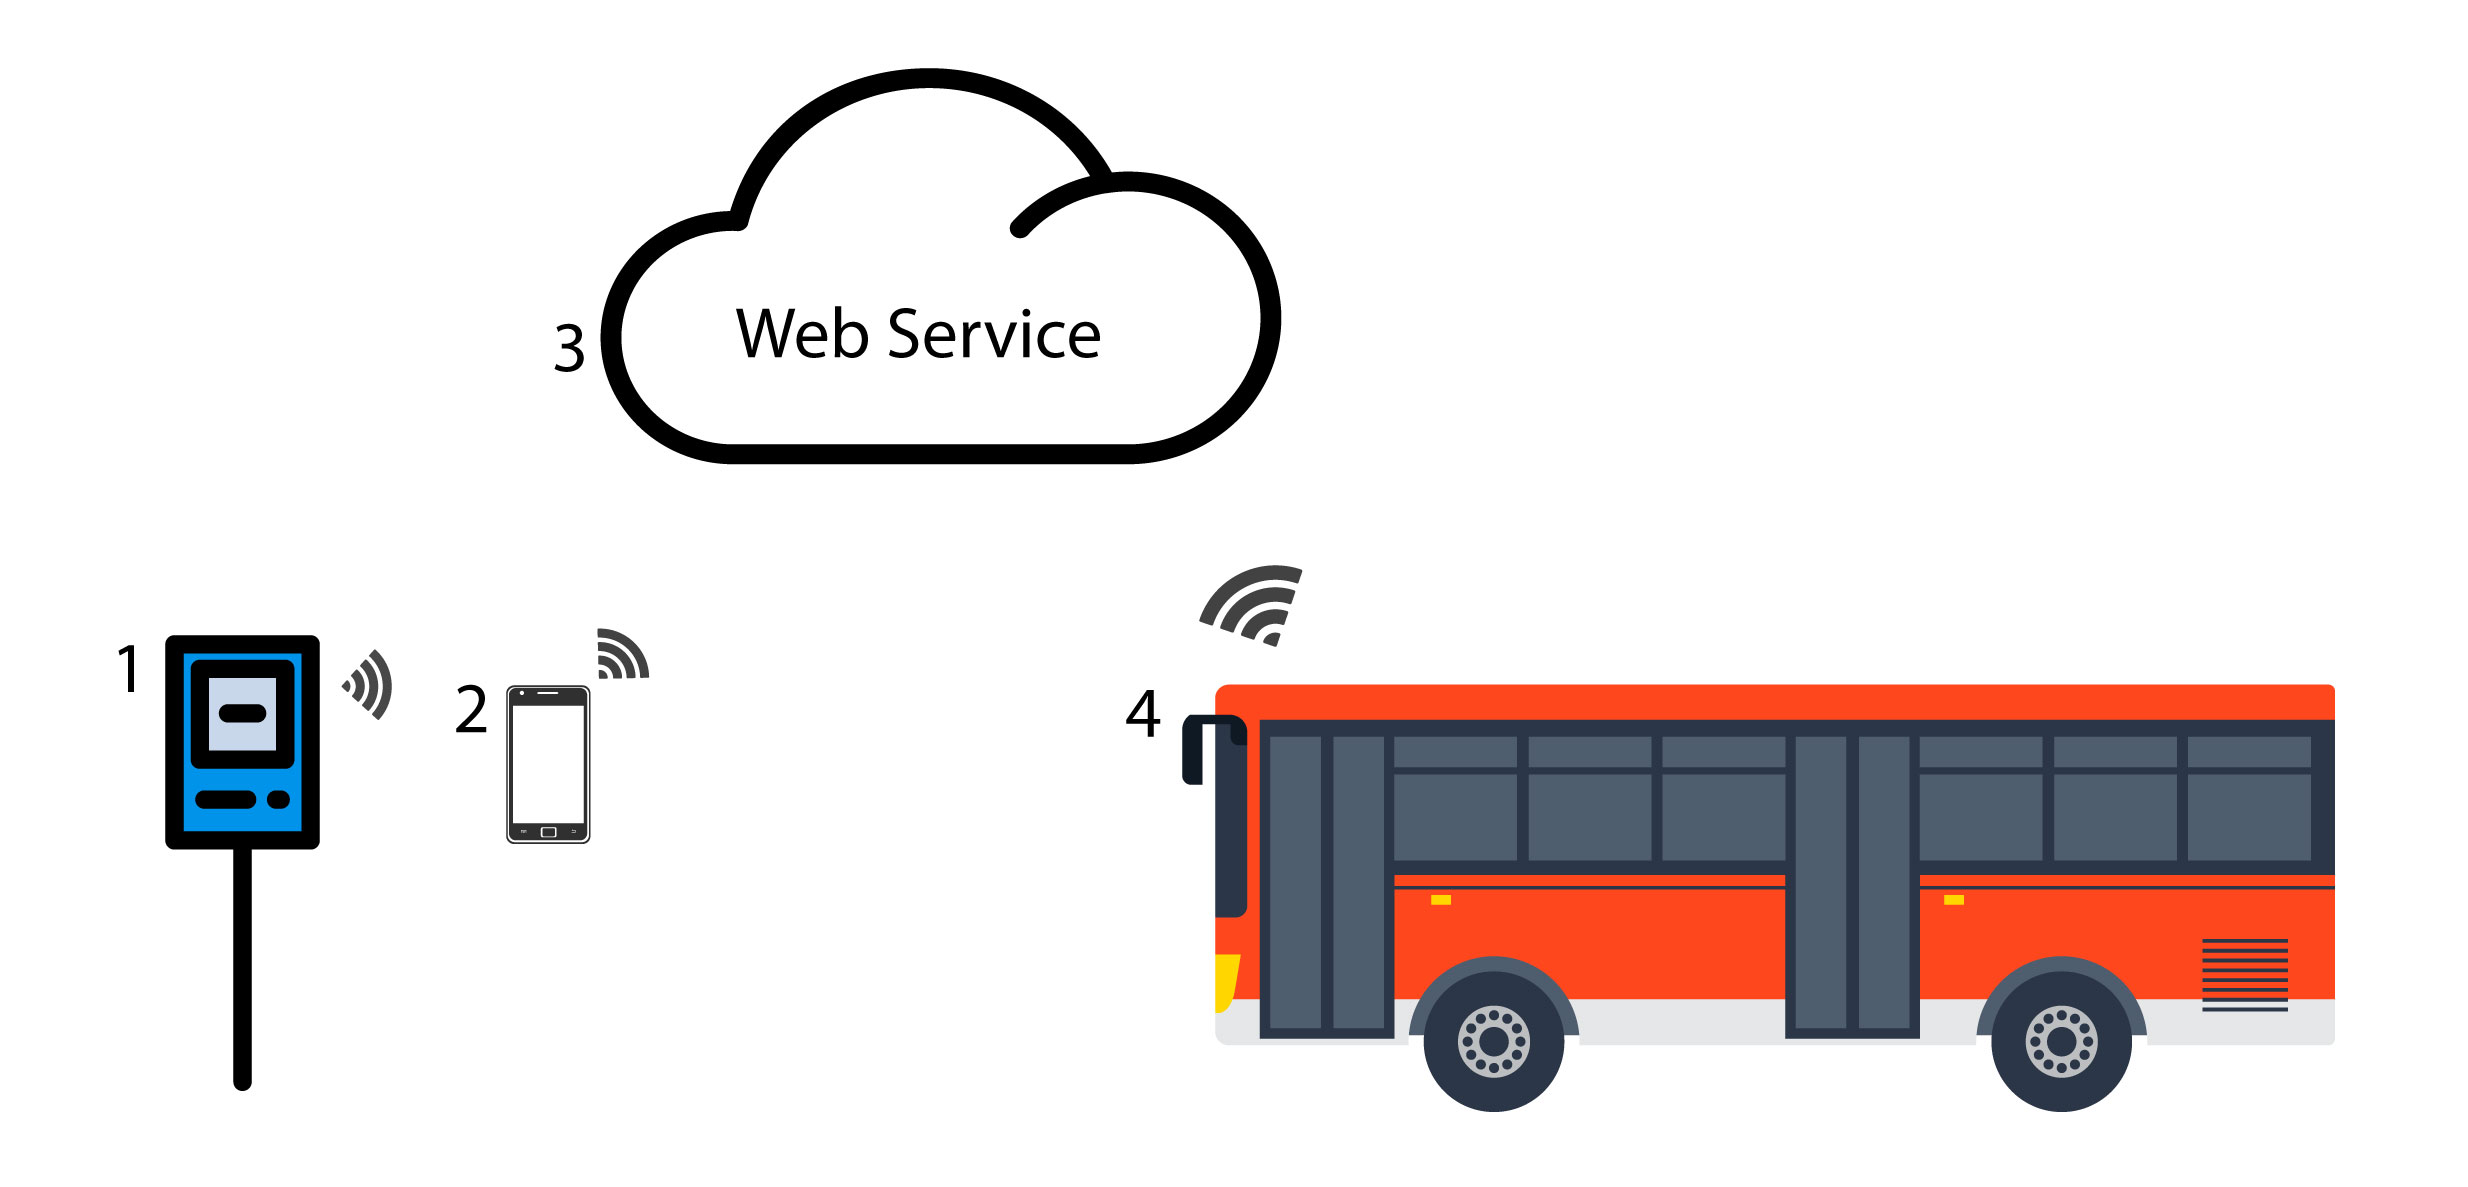
\includegraphics[width=10cm, center]{images/relations_system.jpg}
\caption{Visão geral da comunicação dos componentes.}
\label{Rotulo}
\end{figure}

\subsection{Descrição Funcional}

\subsubsection*{1. Módulo do ponto de ônibus}

Dispositivo localizado em um determinado ponto de parada de ônibus. Emite constantemente um sinal ID para a identificação do ponto que ele se refere.

\subsubsection*{2. Aplicativo para dispositivo móvel}

Aplicativo que irá interagir com o deficiente visual. Sua função é verificar qual \textit{Beacon} está mais próximo para que a API possa saber sua localização, podendo listar, via interface áudio-visual, para o usuário, quais linhas passam no ponto de parada que ele está.

\subsubsection*{3. Web Service}

Sistema que recebe informações do aplicativo e do módulo do ônibus. Tem como objetivo acessar os dados gravados no banco de dados para que possa prover informações de previsão ao aplicativo. Também é responsável por verificar se o módulo do ônibus deve alertar a presença de um usuário no próximo ponto. Além de calcular a previsão de um ônibus até o ponto de parada selecionado.

\subsubsection*{4. Módulo do ônibus}

Dispositivo instalado no ônibus. Mantém comunicação constante com a API para informar sua geolocalização. Verifica ao mesmo tempo a necessidade de alertar o motorista se existe um deficiente visual aguardando no próximo ponto de parada.



\subsection{Representação do Fluxo da Informação}

Aprofundando na parte da comunicação entre os subsistemas, a forma como eles se relacionam e os parâmetros necessários para o funcionamento, seguem a seguinte forma:

\begin{figure}[H]
\centering
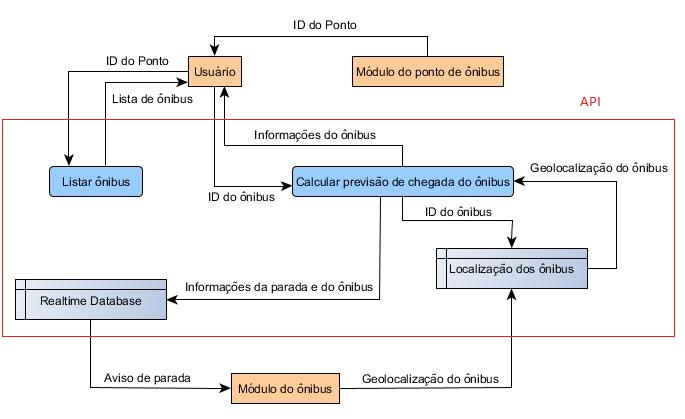
\includegraphics[width=11cm, center]{images/data-flux.jpg}
\caption{Diagrama de fluxo de dados.}
\label{Rotulo}
\end{figure}

\newpage

Para armazenar todas informações necessárias no sistema, foi utilizado o \textit{schema} conforme a Figura \ref{bancodedados}:

\begin{figure}[H]
\centering
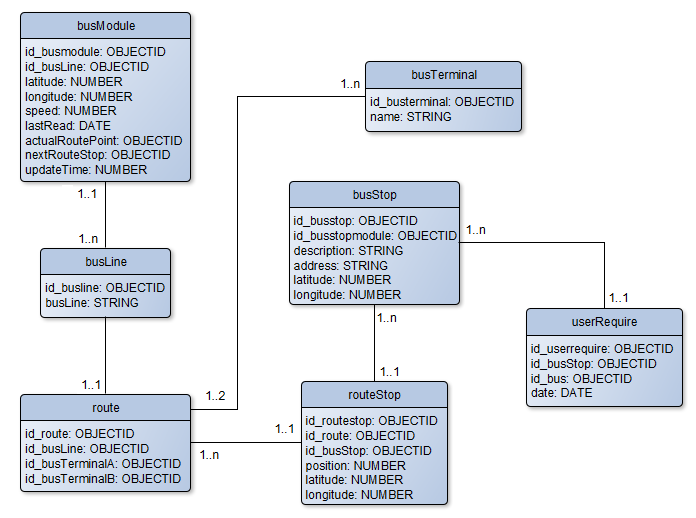
\includegraphics[width=15cm, center]{images/database-api.png}
\caption{Diagrama de banco de dados.}
\label{bancodedados}
\end{figure}

\noindent \textbf{busModule:} Contém as informações de todos módulos dos ônibus.\\
\textbf{busLine:} Contém os registros das linhas de ônibus disponíveis.\\
\textbf{route:} Contém o registro da rota que uma linha de ônibus faz. Nela é possível armazenar o terminal de origem e terminal de destino.\\
\textbf{busTerminal:} Contém os registros de todos terminais de ônibus.\\
\textbf{routePoint:} Cada registro em \textit{route} é associado a N registros em \textit{routePoint}, onde cada \textit{routePoint} representa um ponto geográfico da rota.\\
\textbf{busStop:} Contém todos registros de pontos de parada que existem. \\
\textbf{userRequire:} Contém todos registros de requisições de parada. Quando um usuário solicitar um ônibus, sua solicitação é armazenada nesta \textit{collection}.\\

\newpage

\subsection{Casos de Uso}

\begin{figure}[H]
\centering
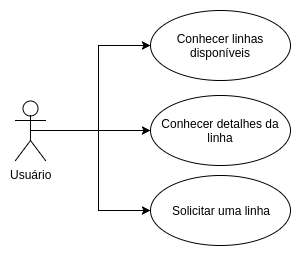
\includegraphics[width=6cm, center]{images/use-case-diagram.png}
\caption{Diagrama de caso de uso.}
\label{Rotulo}
\end{figure}

\subsubsection{Narrativas: Casos de Uso}

Solicitar horário do próximo ônibus da linha e sentido escolhido: este caso de uso acontece quando um usuário solicita qual será a previsão de horário do próximo ônibus, de uma linha e sentido que ele poderá escolher de acordo com o seu ponto de ônibus.

Solicitar parada do ônibus escolhido: este caso de uso é uma extensão do caso de uso “Solicitar horário do próximo ônibus da linha e sentido escolhido”, onde depois de escolher uma linha e sentido ele poderá solicitar a parada do próximo ônibus escolhido.

\newpage

\subsubsection{Diagramas de apoio para compreensão funcional}

\bgroup
\def\arraystretch{1.5}
\begin{table}[H]
\caption{Tabela com caso de uso UC001.}
\centering
\begin{tabular}{|l|l|}
\hline
\multicolumn{2}{|l|}{\textbf{Identificação:} UC001}                                                                 \\ \hline
\multicolumn{2}{|l|}{\textbf{Nome:} Solicitar horário do próximo ônibus}                                            \\ \hline
\multicolumn{2}{|l|}{\textbf{Atores:} Usuário}                                                                      \\ \hline
\multicolumn{2}{|l|}{\textbf{Pré-condições:} O aplicativo precisa ter lido o ID do módulo do ponto de ônibus}       \\ \hline
\multicolumn{2}{|l|}{\textbf{Pós-condições:} Retorno do horário do próximo ônibus e da solicitação de parada}       \\ \hline
\multicolumn{2}{|c|}{\textbf{Fluxo de eventos}}                                                           \\ \hline
\textbf{Ator}                       & \textbf{Sistema}                                                    \\ \hline
\begin{tabular}[c]{@{}l@{}}1. Usuário chega ao ponto de ônibus\end{tabular} & \begin{tabular}[c]{@{}l@{}}2. Sistema lê o ID do ponto de ônibus \\e retorna uma lista de linhas\end{tabular} \\ \hline
\begin{tabular}[c]{@{}l@{}}3. Usuário escolhe uma linha\end{tabular}        & \begin{tabular}[c]{@{}l@{}}4. Informar constantemente \\o horário do ônibus\end{tabular}                      \\ \hline
\multicolumn{2}{|c|}{\textbf{Fluxo alternativo}}                                                          \\ \hline
\multicolumn{2}{|l|}{Não possui fluxo alternativo}                                                        \\ \hline
\end{tabular}
\label{Rotulo}
\end{table}
\egroup

\bgroup
\def\arraystretch{1.5}
\begin{table}[H]
\caption{Tabela com caso de uso UC002.}
\centering
\begin{tabular}{|l|l|}
\hline
\multicolumn{2}{|l|}{\textbf{Identificação:} UC002}                                                                                                                                                                    \\ \hline
\multicolumn{2}{|l|}{\textbf{Nome:} Solicitar parada do ônibus escolhido}                                                                                                                                              \\ \hline
\multicolumn{2}{|l|}{\textbf{Atores:} Usuário}                                                                                                                                                                         \\ \hline
\multicolumn{2}{|l|}{\textbf{Pré-condições:} O usuário precisa ter solicitado o ônibus de uma linha}                                                                                                                   \\ \hline
\multicolumn{2}{|l|}{\textbf{Pós-condições:} Confirmação de parada}                                                                                                                                                    \\ \hline
\multicolumn{2}{|c|}{\textbf{Fluxo de eventos}}                                                                                                                                                                       \\ \hline
\textbf{Ator}                                                                                              & \textbf{Sistema} \\ \hline
\begin{tabular}[c]{@{}l@{}}1. Usuário confirma solicitação \\ de parada no seu ponto\end{tabular} & \begin{tabular}[c]{@{}l@{}}2. Sistema retorna tela de seleção\\  de ponto de ônibus destino\end{tabular} \\ \hline
\multicolumn{2}{|l|}{\textbf{Fluxo alternativo}}                                                                                                                                                                      \\ \hline
\begin{tabular}[c]{@{}l@{}}1.a 1. Usuário cancela \\ solicitação de parada\end{tabular}           & 2. Sistema retorna cancela operação                                                                      \\ \hline
\begin{tabular}[c]{@{}l@{}}3.a 1. Usuário cancela\\  escolha de ponto de ônibus\end{tabular}      & 2. Sistema retorna cancela operação                                                                      \\ \hline
\end{tabular}
\label{Rotulo}
\end{table}
\egroup

\newpage

\begin{figure}[H]
\centering
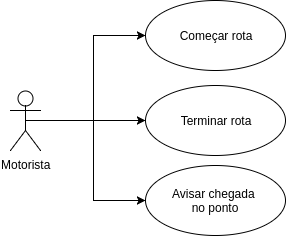
\includegraphics[width=6cm, center]{images/use-case-bus-module.png}
\caption{Diagrama de caso de uso.}
\label{Rotulo}
\end{figure}

\subsubsection{Narrativas: Casos de Uso}

Iniciar uma rota: Este caso de uso acontece quando o motorista inicia sua rota e precisa informar isso ao módulo, para que o dispositivo comece a enviar seus dados de geolocalização para o \textit{Web Service}.

Terminar uma rota: Este caso de uso acontece quando o motorista termina a rota do ônibus e precisa informar isso ao módulo, para que o dispositivo pare de enviar seus dados de geolocalização para o \textit{Web Service}.

Avisar chegada no ponto: Este caso de uso acontece quando um deficiente visual solicitou o ônibus e o motorista está parado no ponto de ônibus. Quando motorista avisa que chegou, é disparado um alerta para o deficiente visual.

\newpage

\subsubsection{Diagramas de apoio para compreensão funcional}

\bgroup
\def\arraystretch{1.5}
\begin{table}[H]
\caption{Tabela com caso de uso UC003.}
\centering
\begin{tabular}{|l|l|}
\hline
\multicolumn{2}{|l|}{\textbf{Identificação:} UC003}                                                                                                                                                                    \\ \hline
\multicolumn{2}{|l|}{\textbf{Nome:} Iniciar uma rota}                                                                                                                                              \\ \hline
\multicolumn{2}{|l|}{\textbf{Atores:} Motorista}                                                                                                                                                                         \\ \hline
\multicolumn{2}{|l|}{\textbf{Pré-condições:} O motorista precisa ter iniciado o módulo}                                                                                                                   \\ \hline
\multicolumn{2}{|l|}{\textbf{Pós-condições:} -}                                                                                                                                                    \\ \hline
\multicolumn{2}{|c|}{\textbf{Fluxo de eventos}}                                                                                                                                                                       \\ \hline
\textbf{Ator}                                                                                              & \textbf{Sistema} \\ \hline
\begin{tabular}[c]{@{}l@{}}1. Usuário confirma o inicio \\da rota\end{tabular} 
& \begin{tabular}[c]{@{}l@{}}2. Módulo começa a enviar dados\\ de geolocalização\end{tabular} 
\\ \hline
 & \begin{tabular}[c]{@{}l@{}}3. Sistema exibe tela com opção \\de parar envio de dados\end{tabular}  \\ \hline
\end{tabular}
\label{Rotulo}
\end{table}
\egroup

\bgroup
\def\arraystretch{1.5}
\begin{table}[H]
\caption{Tabela com caso de uso UC004.}
\centering
\begin{tabular}{|l|l|}
\hline
\multicolumn{2}{|l|}{\textbf{Identificação:} UC004}                                                                                                                                                                    \\ \hline
\multicolumn{2}{|l|}{\textbf{Nome:} Finalizar uma rota}                                                                                                                                              \\ \hline
\multicolumn{2}{|l|}{\textbf{Atores:} Motorista}                                                                                                                                                                         \\ \hline
\multicolumn{2}{|l|}{\textbf{Pré-condições:} O motorista precisa ter iniciado uma rota}                                                                                                                   \\ \hline
\multicolumn{2}{|l|}{\textbf{Pós-condições:} -}                                                                                                                                                    \\ \hline
\multicolumn{2}{|c|}{\textbf{Fluxo de eventos}}                                                                                                                                                                       \\ \hline
\textbf{Ator}                                                                                              & \textbf{Sistema} \\ \hline
\begin{tabular}[c]{@{}l@{}}1. Motorista confirma o fim \\da rota\end{tabular} 
& \begin{tabular}[c]{@{}l@{}}2. Módulo para de enviar dados\\ de geolocalização\end{tabular} 
\\ \hline
 & \begin{tabular}[c]{@{}l@{}}3. Sistema exibe tela com opção \\de iniciar envio de dados\end{tabular}  \\ \hline
\end{tabular}
\label{Rotulo}
\end{table}
\egroup

\newpage

\bgroup
\def\arraystretch{1.5}
\begin{table}[H]
\caption{Tabela com caso de uso UC005.}
\centering
\begin{tabular}{|l|l|}
\hline
\multicolumn{2}{|l|}{\textbf{Identificação:} UC005}                                                                                                                                                                    \\ \hline
\multicolumn{2}{|l|}{\textbf{Nome:} Avisar chegada no ponto}                                                                                                                                              \\ \hline
\multicolumn{2}{|l|}{\textbf{Atores:} Motorista}                                                                                                                                                                         \\ \hline
\multicolumn{2}{|l|}{\textbf{Pré-condições:} O motorista precisa ter iniciado uma rota}                                                                                                                   \\ \hline
\multicolumn{2}{|l|}{\textbf{Pós-condições:} -}                                                                                                                                                    \\ \hline
\multicolumn{2}{|c|}{\textbf{Fluxo de eventos}}                                                                                                                                                                       \\ \hline
\textbf{Ator}                                                                                              & \textbf{Sistema} \\ \hline
\begin{tabular}[c]{@{}l@{}}1. Motorista confirma chegada no \\ponto de ônibus\end{tabular} 
& \begin{tabular}[c]{@{}l@{}}2. Módulo enviar aviso\\ de chegada\end{tabular} 
\\ \hline
 & \begin{tabular}[c]{@{}l@{}}3. Sistema exibe tela com opção \\de parar envio de dados\end{tabular}  \\ \hline
\end{tabular}
\label{Rotulo}
\end{table}
\egroup

\newpage

\subsection{Interfaces com Sistema}

Neste tópico, serão apresentados as telas criadas tanto para o aplicativo, quanto para o módulo do ônibus.

\subsubsection{Aplicativo}

\subsubsubsection{Busca por um ponto próximo}

\begin{figure}[H]
\centering
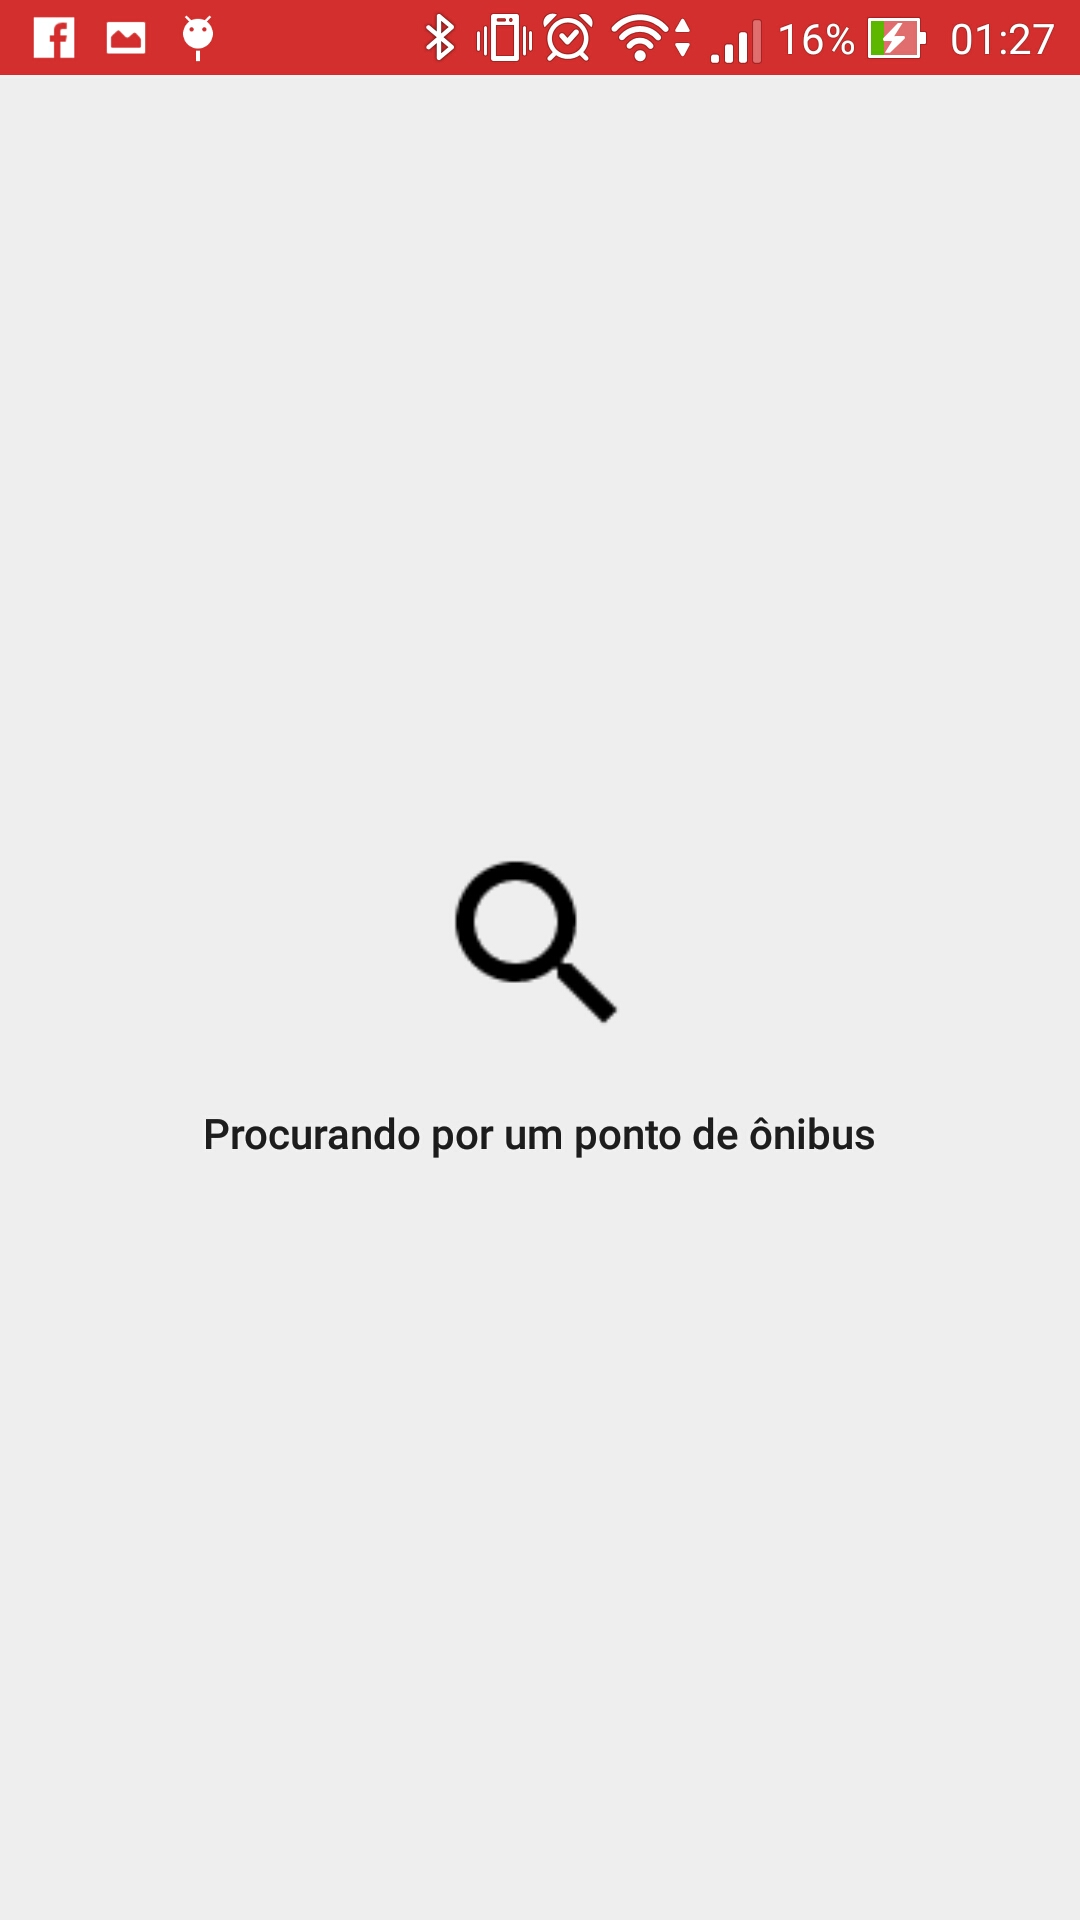
\includegraphics[width=5cm, center]{images/beacon_searching_bus_stop}
\caption{Tela do aplicativo ao buscar por um ponto de ônibus próximo.}
\label{Rotulo}
\end{figure}

\begin{table}[H]
\caption{Descrição dos elementos da tela de busca por ponto de ônibus próximo.}
\centering
\begin{tabular}{@{}|c|c|c|c|c|@{}}
\hline
Número & 
Nome & 
Descrição & 
Requisitos & 
Grupo\\ \hline
1 & \begin{tabular}[c]{@{}c@{}}Símbolo da busca \\ do ponto de ônibus\end{tabular} & \begin{tabular}[c]{@{}c@{}}Indica que o aplicativo \\ está procurando um \\ ponto de ônibus\end{tabular}                  & -                     & Imagem e texto \\ \hline
2 & Áudio sobre busca & \begin{tabular}[c]{@{}c@{}}Indica ao usuário que \\ está sendo feito uma \\ busca por algum \\ ponto próximo\end{tabular} & Função Talkback ativa & Áudio\\ \hline
\end{tabular}
\label{Rotulo}
\end{table}

\newpage

\subsubsubsection{Busca por um ponto na API}

\begin{figure}[H]
\centering
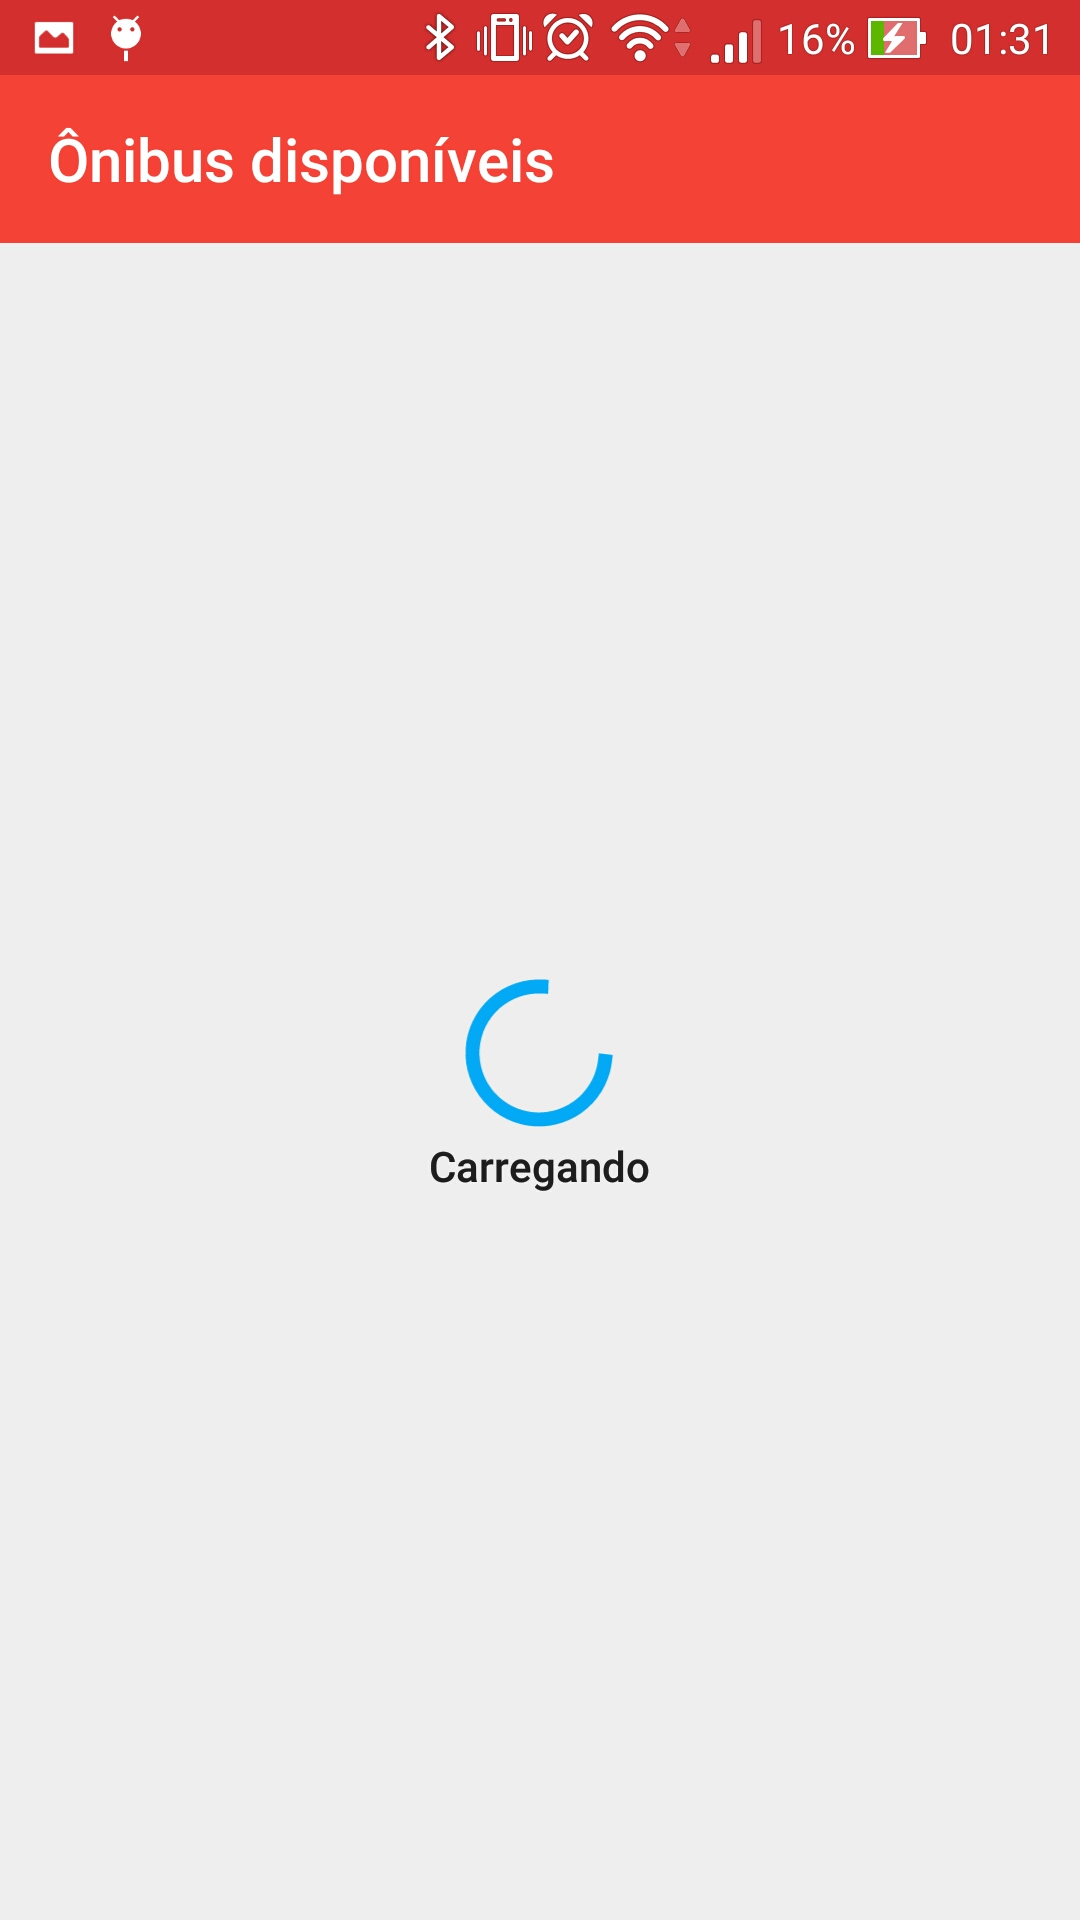
\includegraphics[width=5cm, center]{images/beacon_searching_list_bus}
\caption{Tela do aplicativo ao buscar por um ponto de ônibus na API.}
\label{Rotulo}
\end{figure}

\begin{table}[H]
\caption{Descrição dos elementos da tela de busca por ponto de ônibus na API.}
\centering
\begin{tabular}{@{}|c|c|c|c|c|@{}}
\hline
Número & 
Nome & 
Descrição & 
Requisitos & 
Grupo\\ \hline
1 & \begin{tabular}[c]{@{}c@{}}Símbolo da busca \\ das linhas de ônibus\end{tabular} & \begin{tabular}[c]{@{}c@{}}Indica que o \\ aplicativo \\ procura as\\linhas de ônibus\end{tabular} & \begin{tabular}[c]{@{}c@{}}O sistema deve ter\\detectado um ponto\\de ônibus\end{tabular} & Imagem e texto \\ \hline
2 & Áudio sobre busca & \begin{tabular}[c]{@{}c@{}}Indica ao usuário\\ que está sendo \\feito uma busca\\ dos ônibus disponíveis\end{tabular} & Função Talkback ativa & Áudio\\ \hline
\end{tabular}
\label{Rotulo}
\end{table}

\newpage

\subsubsubsection{Lista de ônibus disponíveis}

\begin{figure}[H]
\centering
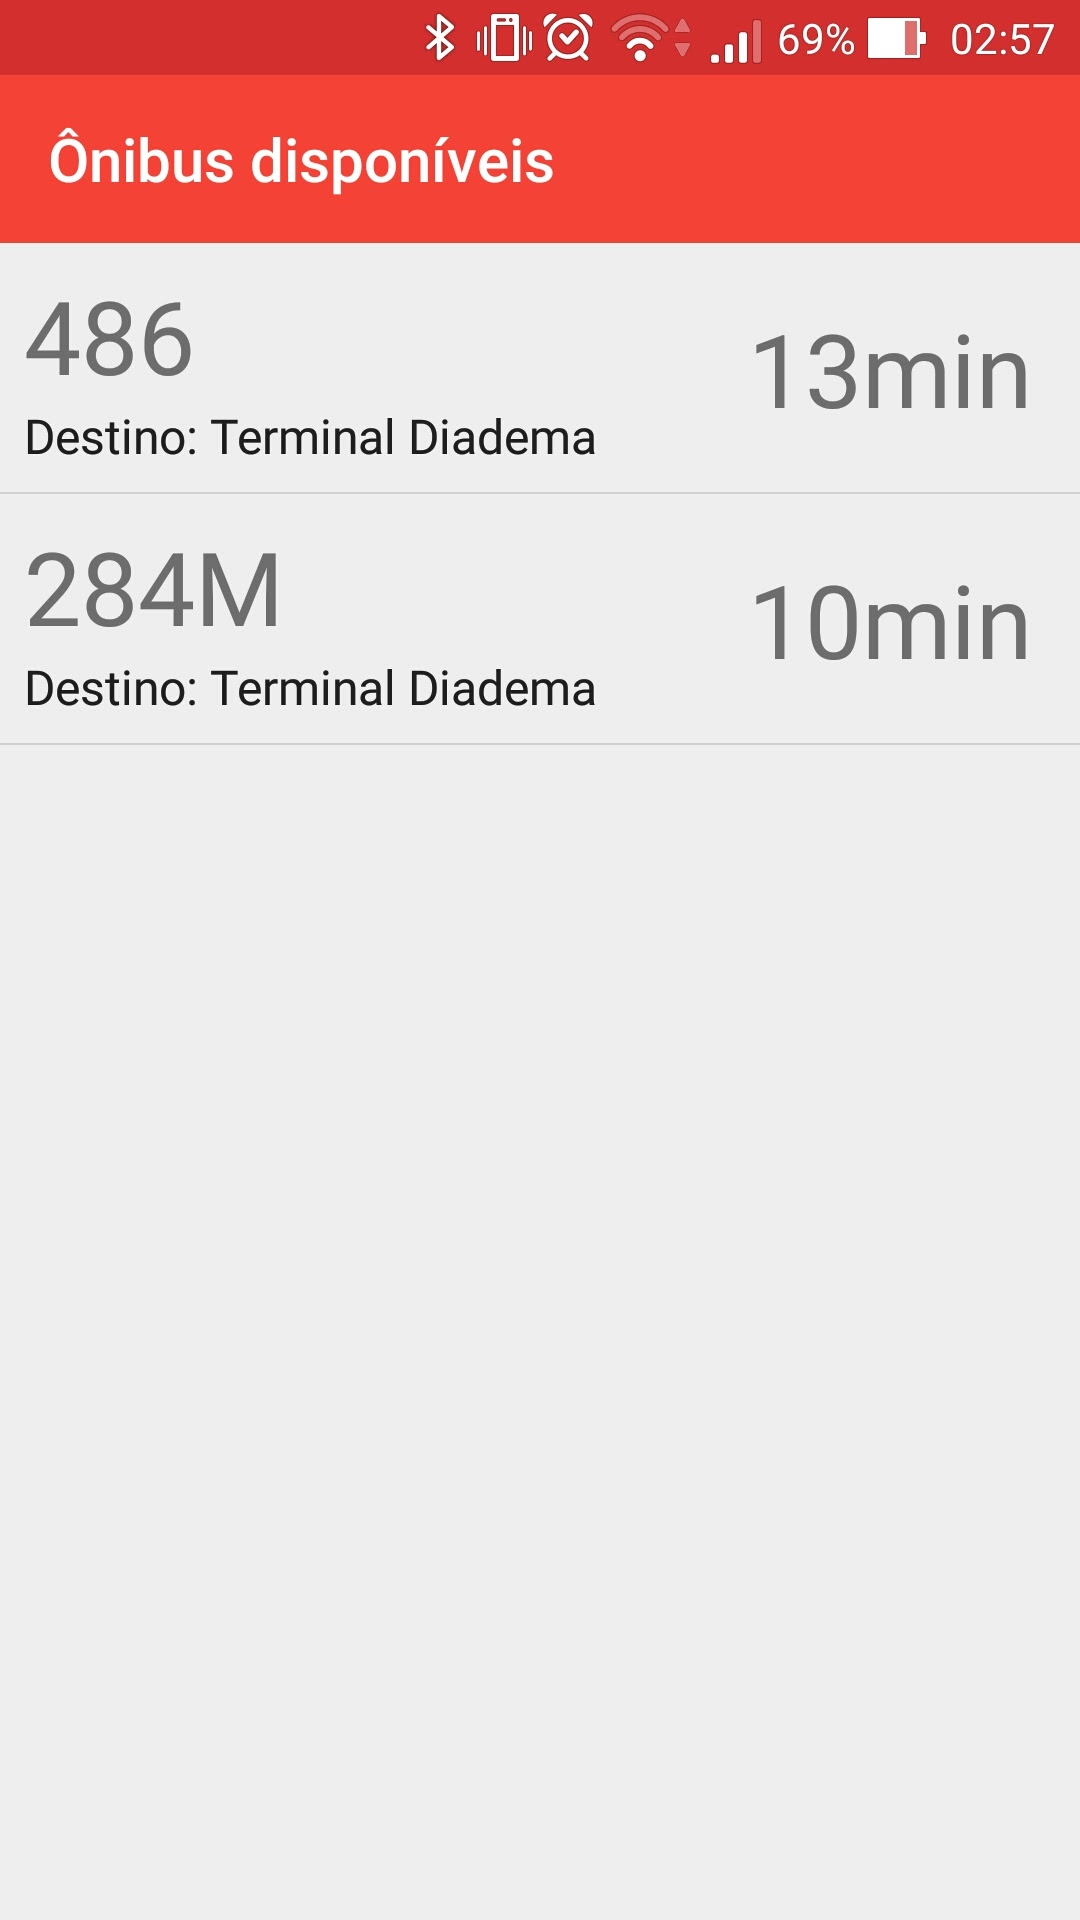
\includegraphics[width=5cm, center]{images/beacon-list-bus}
\caption{Tela do aplicativo com ônibus disponíveis.}
\label{Rotulo}
\end{figure}

\begin{table}[H]
\caption{Descrição dos elementos da tela de busca por ponto de ônibus na API.}
\centering
\begin{tabular}{@{}|c|c|c|c|c|@{}}
\hline
Número & 
Nome & 
Descrição & 
Requisitos & 
Grupo\\ \hline
1 & Lista de linhas & \begin{tabular}[c]{@{}c@{}}Lista de linhas\\ que o usuário\\ pode escolher\end{tabular} & \begin{tabular}[c]{@{}c@{}}Ter recebido uma\\ lista da API\end{tabular} & Botão \\ \hline
2 & \begin{tabular}[c]{@{}c@{}}Áudio sobre escolha\\ de um item\end{tabular} & \begin{tabular}[c]{@{}c@{}}Indica que a lista\\ de ônibus já está\\ disponível\end{tabular} & Função Talkback ativa & Áudio\\ \hline
\end{tabular}
\label{Rotulo}
\end{table}

\newpage

\subsubsubsection{Detalhes do ônibus}

\begin{figure}[H]
\centering
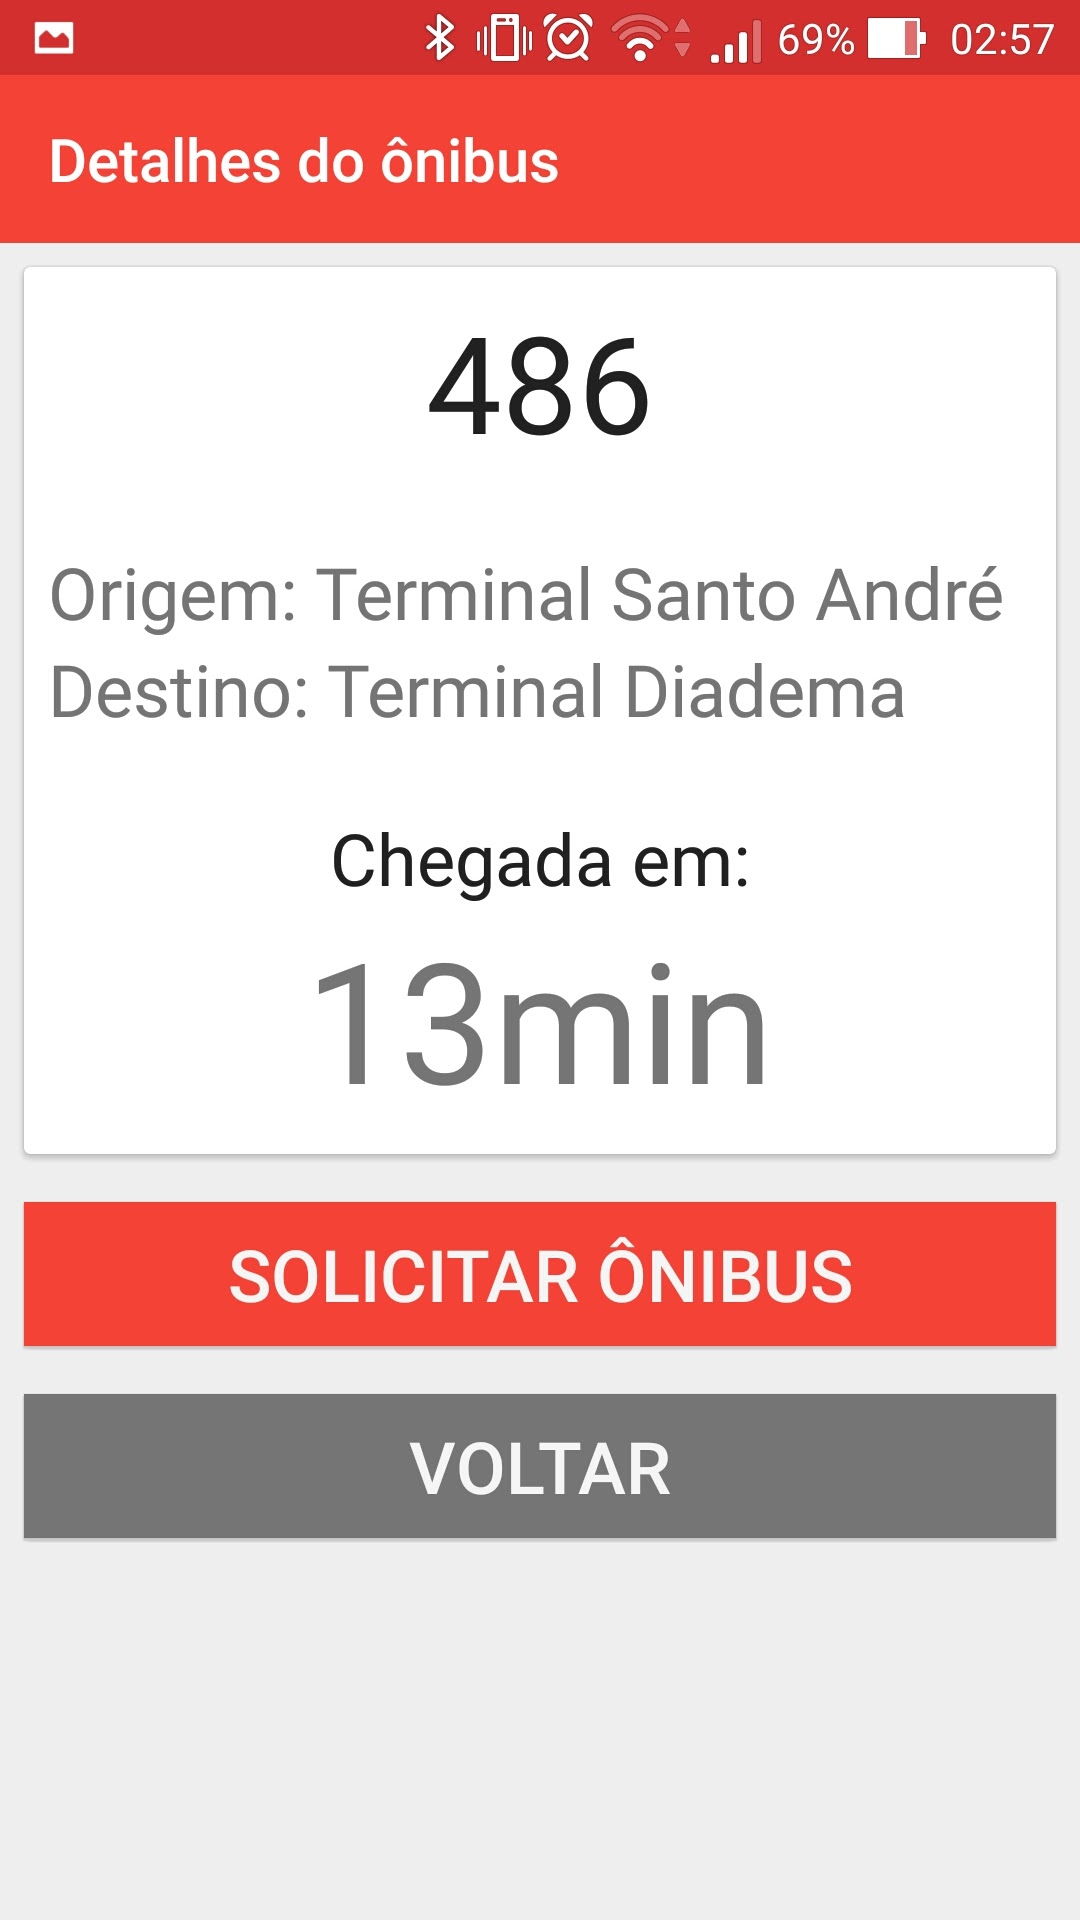
\includegraphics[width=5cm, center]{images/beacon-detail-bus}
\caption{Tela do aplicativo com detalhes de um ônibus.}
\label{Rotulo}
\end{figure}

\begin{table}[H]
\caption{Descrição dos elementos da tela de detalhes do ônibus.}
\centering
\begin{tabular}{@{}|c|c|c|c|c|@{}}
\hline
Número                  & Nome                                  & Descrição                                                                                                                                     & Requisitos                                                                              & Grupo                      \\ \hline
\multicolumn{1}{|c|}{1} & \multicolumn{1}{c|}{Linha X1}         & \multicolumn{1}{c|}{Mostra a linha selecionada}                                                                                               & \multicolumn{1}{c|}{\begin{tabular}[c]{@{}c@{}}Receber previsão \\ da API\end{tabular}} & \multicolumn{1}{c|}{Texto} \\ \hline
\multicolumn{1}{|c|}{2} & \multicolumn{1}{c|}{Origem}           & \multicolumn{1}{c|}{Exibe o ponto inicial da linha}                                                                                           & \multicolumn{1}{c|}{\begin{tabular}[c]{@{}c@{}}Receber previsão \\ da API\end{tabular}} & \multicolumn{1}{c|}{Texto} \\ \hline
\multicolumn{1}{|c|}{3} & \multicolumn{1}{c|}{Destino}          & \multicolumn{1}{c|}{Exibe o ponto final da linha}                                                                                             & \multicolumn{1}{c|}{\begin{tabular}[c]{@{}c@{}}Receber previsão \\ da API\end{tabular}} & \multicolumn{1}{c|}{Texto} \\ \hline
\multicolumn{1}{|c|}{4} & \multicolumn{1}{c|}{Chegada em}       & \multicolumn{1}{c|}{\begin{tabular}[c]{@{}c@{}}Exibe a previsão de\\  chegada da linha\end{tabular}}                                          & \multicolumn{1}{c|}{\begin{tabular}[c]{@{}c@{}}Receber previsão \\ da API\end{tabular}} & \multicolumn{1}{c|}{Texto} \\ \hline
\multicolumn{1}{|c|}{5} & \multicolumn{1}{c|}{Voltar}           & \multicolumn{1}{c|}{Volta para a seleção de linhas}                                                                                           & \multicolumn{1}{c|}{\begin{tabular}[c]{@{}c@{}}Receber previsão\\  da API\end{tabular}} & \multicolumn{1}{c|}{Botão} \\ \hline
\multicolumn{1}{|c|}{6} & \multicolumn{1}{c|}{Solicitar ônibus} & \multicolumn{1}{c|}{\begin{tabular}[c]{@{}c@{}}Solicita que o ônibus\\  pare no seu\\  ponto e acionar o \\ acompanhamento dele\end{tabular}} & \multicolumn{1}{c|}{\begin{tabular}[c]{@{}c@{}}Receber previsão \\ da API\end{tabular}} & \multicolumn{1}{c|}{Botão} \\ \hline
7                       & Áudio sobre previsão                  & \begin{tabular}[c]{@{}c@{}}Alerta ao usuário a\\  previsão do ônibus\end{tabular}                                                             & \begin{tabular}[c]{@{}c@{}}Receber previsão \\ da API\end{tabular}                      & Áudio                      \\ \hline
\end{tabular}
\label{Rotulo}
\end{table}

\newpage

\subsubsubsection{Aguardando um ônibus}

\begin{figure}[H]
\centering
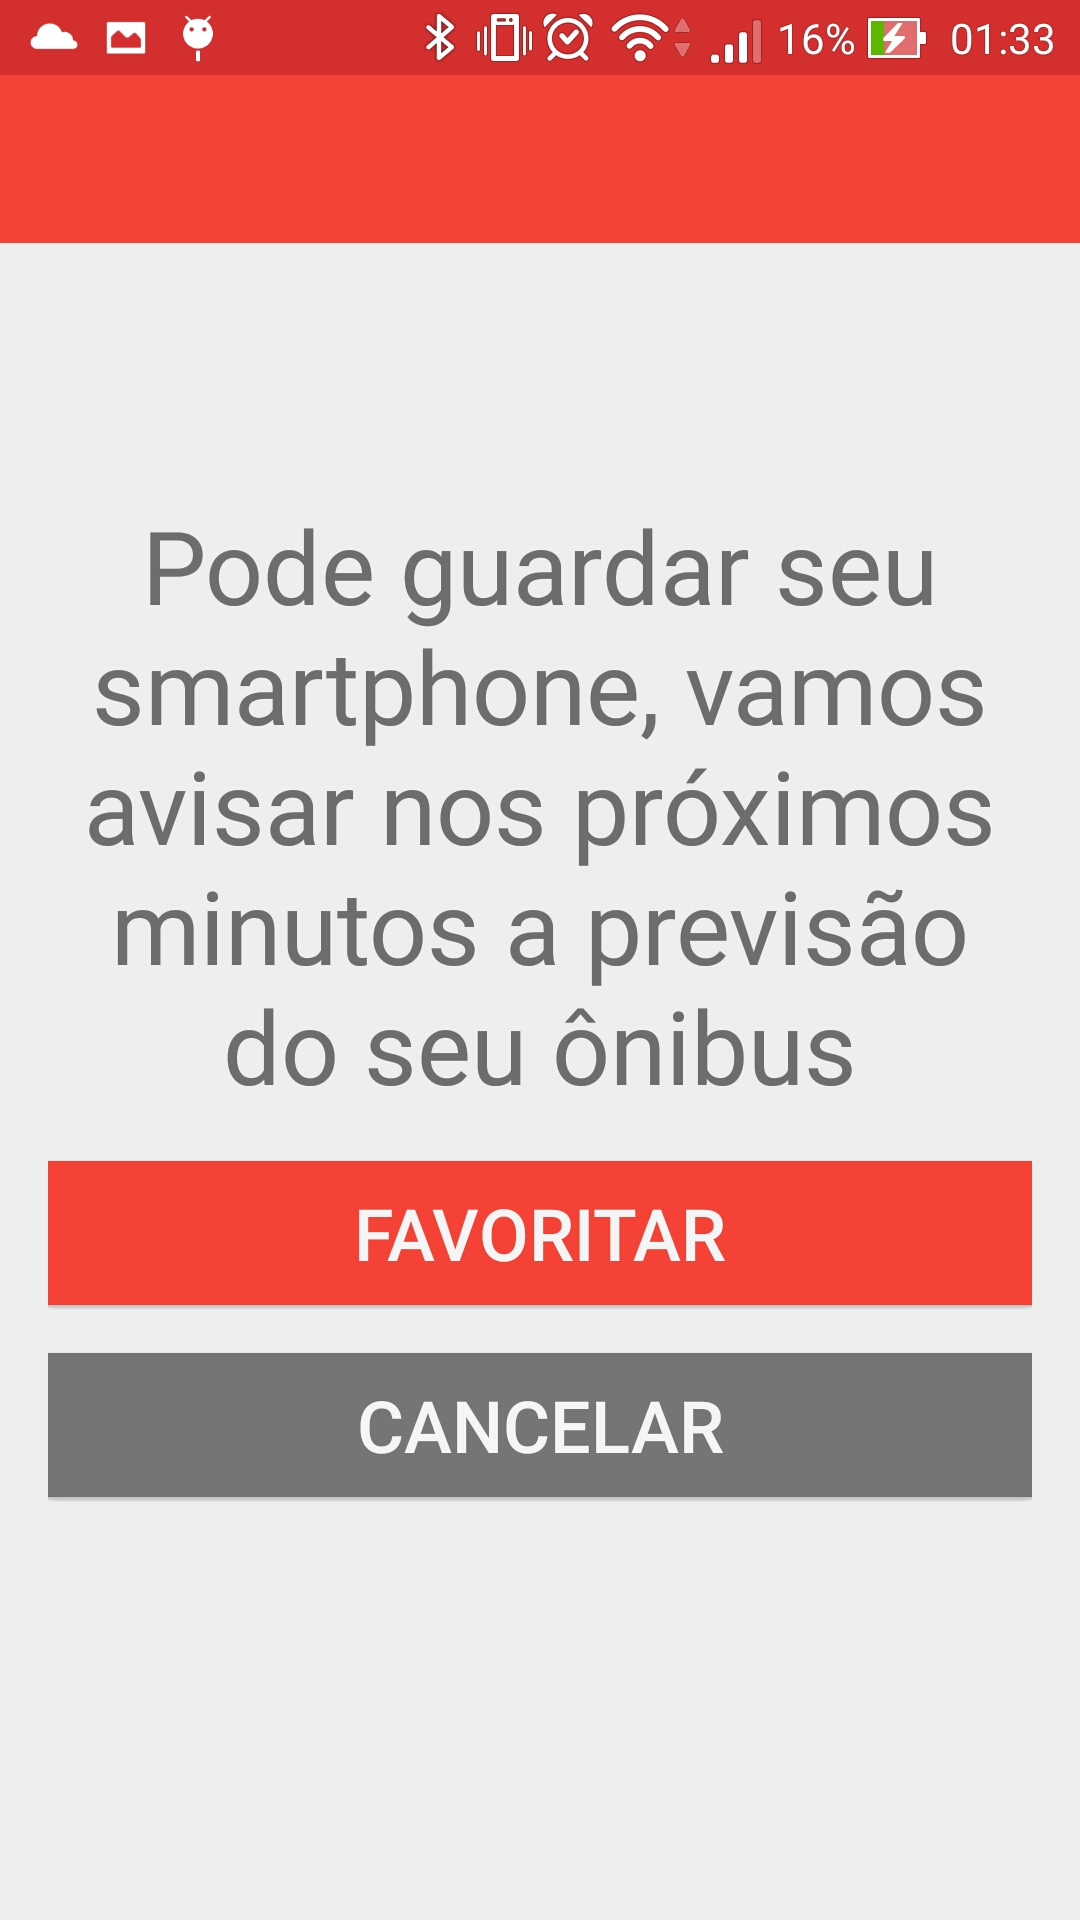
\includegraphics[width=5cm, center]{images/beacon_waiting_bus}
\caption{Tela do aplicativo sobre a solicitação de um ônibus.}
\label{Rotulo}
\end{figure}

\begin{table}[H]
\caption{Descrição dos elementos da tela sobre a solicitação de um ônibus.}
\centering
\begin{tabular}{|c|c|c|c|c|}
\hline
Número & Nome                                                                    & Descrição                                                                                                              & Requisitos                                                                                                                              & Grupo \\ \hline
1
 & \begin{tabular}[c]{@{}c@{}}Informação \\ de previsão\end{tabular}       & \begin{tabular}[c]{@{}c@{}}O sistema irá \\ informar o \\ usuário até a \\ chegada do ônibus\end{tabular}              & \begin{tabular}[c]{@{}c@{}}Ter selecionado botão \\ Solicitar ônibus\end{tabular}                                                       & Texto \\ \hline
2      & Favoritar                                                               & \begin{tabular}[c]{@{}c@{}}Adiciona ônibus\\ como favorito\end{tabular}                                                & \begin{tabular}[c]{@{}c@{}}O ônibus não pode \\ estar cadastrado \\ como favorito. \\ Caso esteja o \\ botão não é exibido\end{tabular} & Botão \\ \hline
3      & Cancelar                                                                & \begin{tabular}[c]{@{}c@{}}Cancela o acompanhamento \\ do ônibus e solicita \\ que não pare mais no ponto\end{tabular} & \begin{tabular}[c]{@{}c@{}}Ter selecionado botão\\  Solicitar ônibus\end{tabular}                                                       & Botão \\ \hline
4      & \begin{tabular}[c]{@{}c@{}}Áudio sobre o \\ acompanhamento\end{tabular} & \begin{tabular}[c]{@{}c@{}}Informa ao usuário \\ que está sendo \\ feito o acompanhamento \\ do ônibus\end{tabular}    & \begin{tabular}[c]{@{}c@{}}Ter escolhido acompanhar \\ um ônibus.\\ Função Talkback ativa\end{tabular}                                  & Áudio \\ \hline
\end{tabular}
\label{Rotulo}
\end{table}

\newpage

\subsubsection{Módulo do ônibus}

\subsubsubsection{Carregando Informações}

\begin{figure}[H]
\centering
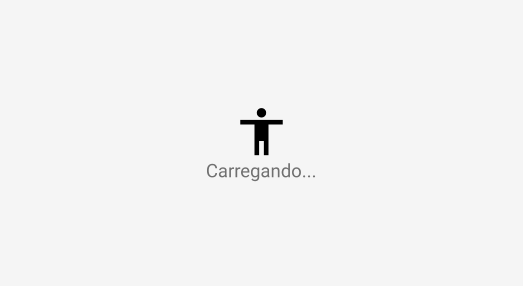
\includegraphics[width=15cm, center]{images/bus-tracker-loading}
\caption{Tela do módulo do ônibus quando está carregando informações.}
\label{Rotulo}
\end{figure}

\begin{table}[H]
\caption{Descrição dos elementos da tela sobre estar carregando informações.}
\centering
\begin{tabular}{|c|c|c|c|c|}
\hline
Número & Nome                                                                    & Descrição                                                                                                              & Requisitos                                                                                                                              & Grupo \\ 
\hline 
\begin{tabular}[c]{@{}c@{}}1\end{tabular}  & \begin{tabular}[c]{@{}c@{}}Mensagem\end{tabular}  & \begin{tabular}[c]{@{}c@{}}Informa que está carregando informações \\do servidor\end{tabular}  & \begin{tabular}[c]{@{}c@{}}Ter iniciado o sistema\end{tabular}  & \begin{tabular}[c]{@{}c@{}}Texto\end{tabular}  \\ 
\hline 
\end{tabular} 
\label{Rotulo}
\end{table}

\newpage

\subsubsubsection{Aguardando iniciar a rota}

\begin{figure}[H]
\centering
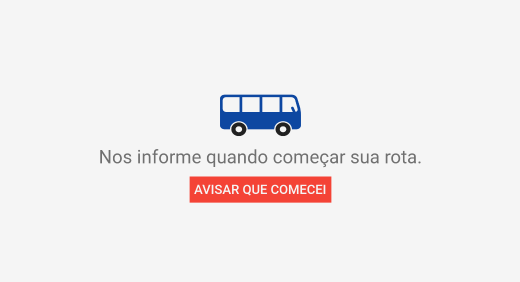
\includegraphics[width=15cm, center]{images/bus-tracker-waiting-start-route}
\caption{Tela do módulo do ônibus aguardando motorista iniciar rota.}
\label{Rotulo}
\end{figure}

\begin{table}[H]
\caption{Descrição dos elementos da tela sobre começar uma rota.}
\centering
\begin{tabular}{|c|c|c|c|c|}
\hline
Número & Nome                                                                    & Descrição                                                                                                              & Requisitos                                                                                                                              & Grupo \\
\hline 
\begin{tabular}[c]{@{}c@{}}1\end{tabular} 
& \begin{tabular}[c]{@{}c@{}}Informação para\\ começar rota\end{tabular} 
& \begin{tabular}[c]{@{}c@{}}Informar que precisa avisar \\ quando começar a rota\end{tabular} 
& \begin{tabular}[c]{@{}c@{}}-\end{tabular} & \begin{tabular}[c]{@{}c@{}}Texto\end{tabular} \\ 
\hline 
\begin{tabular}[c]{@{}c@{}}2\end{tabular} 
& \begin{tabular}[c]{@{}c@{}}Começar rota\end{tabular} 
& \begin{tabular}[c]{@{}c@{}}Começar rotina de envio da posição\end{tabular} 
& \begin{tabular}[c]{@{}c@{}}-\end{tabular} 
& \begin{tabular}[c]{@{}c@{}}Botão\end{tabular} \\ 
\hline 
\end{tabular} 
\label{Rotulo}
\end{table}

\newpage

\subsubsubsection{Realizando uma rota}

\begin{figure}[H]
\centering

\includegraphics[width=15cm, center]{images/bus-tracker-in-route}
\caption{Tela do módulo do ônibus quando motorista está fazendo a rota.}
\label{Rotulo}
\end{figure}

\begin{table}[H]
\caption{Descrição dos elementos da tela sobre terminar uma rota.}
\centering
\begin{tabular}{|c|c|c|c|c|}
\hline
Número & Nome                                                                    & Descrição                                                                                                              & Requisitos                                                                                                                              & Grupo \\
\hline 
\begin{tabular}[c]{@{}c@{}}1\end{tabular} 
& \begin{tabular}[c]{@{}c@{}}Informação sobre\\término da rota\end{tabular} 
& \begin{tabular}[c]{@{}c@{}}Informar que precisa avisar \\ quando terminar a rota\end{tabular} 
& \begin{tabular}[c]{@{}c@{}}Ter iniciado\\uma rota\end{tabular} & \begin{tabular}[c]{@{}c@{}}Texto\end{tabular} \\ 
\hline 
\begin{tabular}[c]{@{}c@{}}2\end{tabular} 
& \begin{tabular}[c]{@{}c@{}}Terminar rota\end{tabular} 
& \begin{tabular}[c]{@{}c@{}}Terminar rotina de envio da posição\end{tabular} 
& \begin{tabular}[c]{@{}c@{}}Ter iniciado\\uma rota\end{tabular} 
& \begin{tabular}[c]{@{}c@{}}Botão\end{tabular} \\ 
\hline 
\end{tabular} 
\label{Rotulo}
\end{table}

\newpage

\subsubsubsection{Aviso para parar no próximo ponto}

\begin{figure}[H]
\centering

\includegraphics[width=15cm, center]{images/bus-tracker-needs-to-stop}
\caption{Tela do módulo do ônibus quando motorista precisar parar no próximo ponto.}
\label{Rotulo}
\end{figure}

\begin{table}[H]
\caption{Descrição dos elementos da tela sobre terminar uma rota.}
\centering
\begin{tabular}{|c|c|c|c|c|}
\hline
Número & Nome                                                                    & Descrição                                                                                                              & Requisitos                                                                                                                              & Grupo \\
\hline 
\begin{tabular}[c]{@{}c@{}}1\end{tabular} 
& \begin{tabular}[c]{@{}c@{}}Símbolo de alerta\\ para parar\end{tabular} 
& \begin{tabular}[c]{@{}c@{}}Informar que precisa parar \\ no próximo ponto\end{tabular} 
& \begin{tabular}[c]{@{}c@{}}Servidor informar\\ a necessidade\end{tabular} & \begin{tabular}[c]{@{}c@{}}Imagem e Texto\end{tabular} \\ 
\hline 
\begin{tabular}[c]{@{}c@{}}2\end{tabular} 
& \begin{tabular}[c]{@{}c@{}}Informar chegada\end{tabular} 
& \begin{tabular}[c]{@{}c@{}}Envia informação que\\ chegou no ponto\end{tabular} 
& \begin{tabular}[c]{@{}c@{}}Ter chegado no\\ ponto\end{tabular} 
& \begin{tabular}[c]{@{}c@{}}Botão\end{tabular} \\ 
\hline 
\end{tabular} 
\label{Rotulo}
\end{table}

\newpage

\section{Módulo do Ponto de Ônibus}

\subsection{Hardware}

\begin{enumerate}
\item HM-10 - Bluetooth 4.0 BLE module
\item Arduino Uno
\end{enumerate}

\subsection{Software}

\begin{itemize}
\item Arduino IDE 1.8.3 ou superior, encontrado em <https://www.arduino.cc/en/main/software>. 
\end{itemize}

\subsection{Configuração}

Para configurar o módulo HM-10 utilizamos o Arduino como ponte. Para realizar tais configurações, foi montado o circuito conforme a Figura \ref{beacon}.

\begin{figure}[H]
\centering
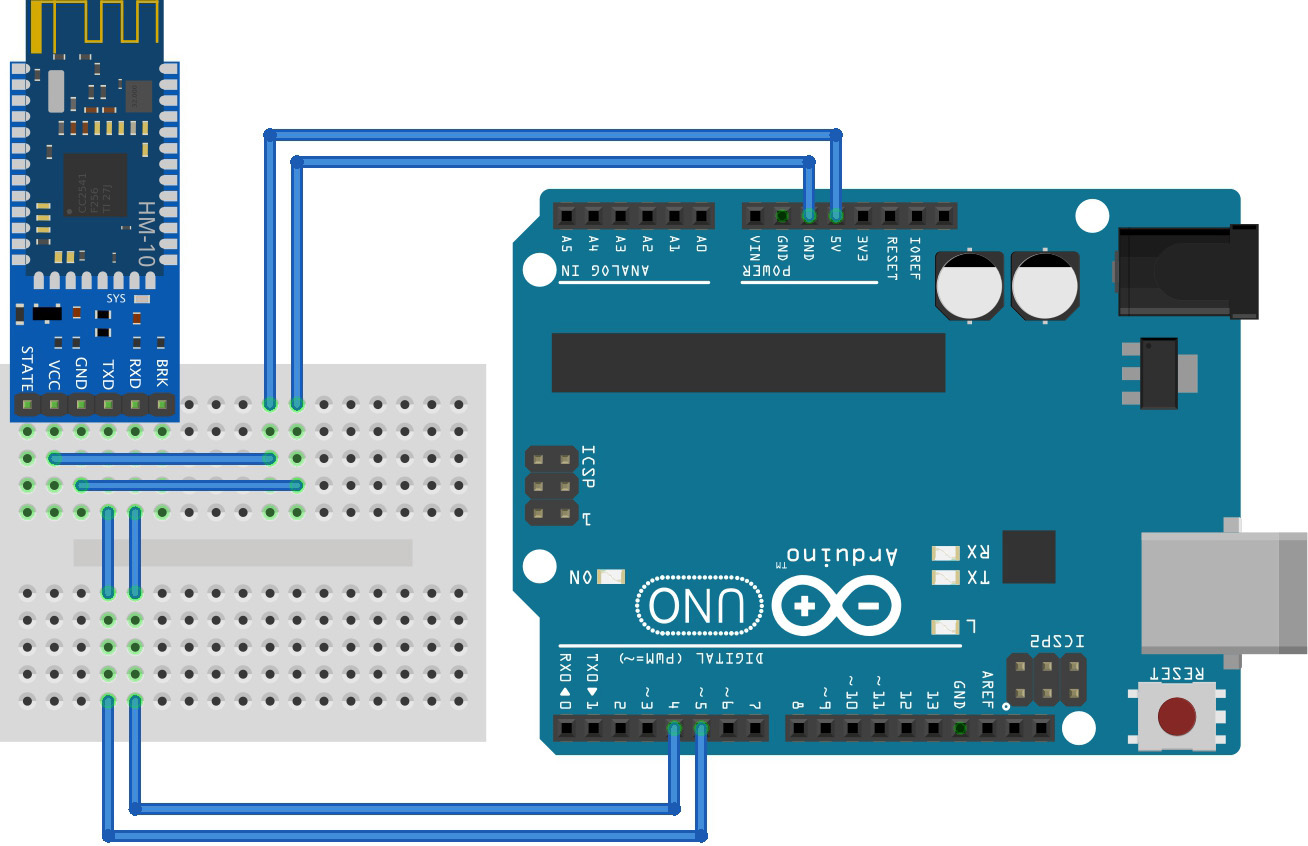
\includegraphics[width=10cm, center]{images/arduino-hm10}
\caption{Configurando o módulo \textit{Bluetooth} HM-10 via Arduino UNO.}
\label{beacon}
\end{figure}

Após conectar o Arduino ao computador, foi utilizado sua \textit{IDE} para escrever o código, que está no apêndice A. No código do Arduino, foi estabelecido uma comunicação serial com o módulo HM-10 para enviar os comandos AT necessários. Esses comandos são para otimizar o uso da bateria e ativar a função \textit{Beacon} do módulo. A seguir, a descrição dos comandos.

\begin{tabular}{|c|c|}
\hline 
Código & Descrição \\ 
\hline 
AT+RENEW & Coloca nos padrões de fábrica \\ 
\hline 
AT+RESET & Reinicia para aplicar os padrões de fábrica \\ 
\hline 
AT+MARJ0xNNNN & Define o valor Marjor \\ 
\hline 
AT+MINO0xNNNN & Define o valor Minor \\ 
\hline 
AT+NAMEMeuBeacon & Define o nome do dispositivo \\ 
\hline 
AT+ADVI5 & Define tempo de envio. 5 = 546.25 millisegundos \\ 
\hline 
AT+ADTY3 & Define como não pareável \\ 
\hline 
AT+IBEA1 & Habilita como \textit{Beacon} \\ 
\hline 
AT+DELO2 & Configura para apenas emitir sinal \\ 
\hline 
AT+PWRM0 & Habilita função auto-sleep para economizar energia \\ 
\hline 
AT+RESET & Reinicia para aplicar as configurações \\ 
\hline 
\end{tabular} 

Após configurado, o módulo pode ser ligado em uma bateria 3,3v para utilização.

\newpage

\section{Módulo do Ônibus}

\subsection{Hardware}

\begin{itemize}
\item Raspberry Pi 3
\item Tela LCD 7" \textit{Touch Screen}
\item NEO u-blox 6 GPS Modules
\end{itemize}

\begin{figure}[H]
\centering
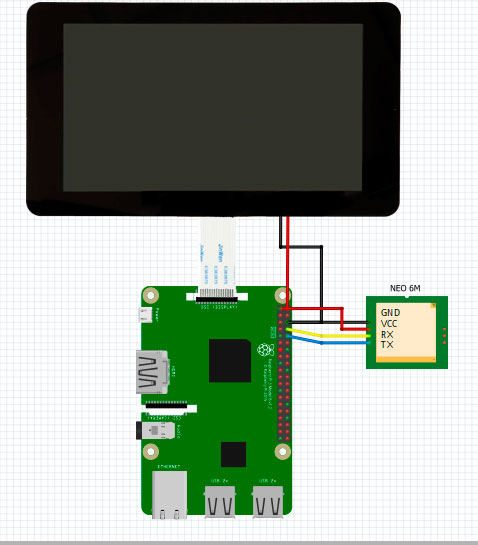
\includegraphics[width=10cm, center]{images/schematic-bus-module}
\caption{Hardware do módulo do ônibus.}
\label{Rotulo}
\end{figure}

\subsubsection{Intel Edison}

\begin{figure}[H]
\centering
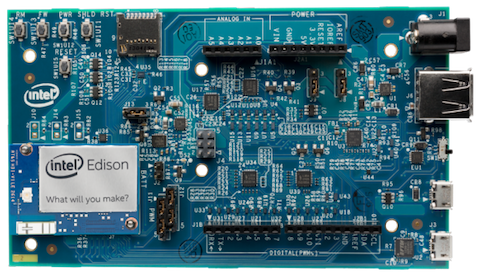
\includegraphics[width=10cm, center]{images/intel-edison-arduino-kit}
\caption{Intel Edison}
\fonte{\citeauthor{edisonimage}}
\label{Rotulo}
\end{figure}

Inicialmente foi adotado o \textit{Intel Edison} com placa de expansão Arduino. Foi escolhido devido a fácil acesso a um exemplar e ótimo hardware. Ele conta com \textit{WiFi}, \textit{Bluetooth}, portas I/O, processador Intel Atom de 500 MHz, 1GB de memória RAM DDR3 e 4GB eMMC. \\

Sua utilização foi fácil e não obtivemos nenhuma dificuldade em instalar o sistema escolhido.


Problemas encontrados em adotar como solução:
\\

\textbf{Preço}

Embora tenha um ótimo hardware e uma empresa séria por trás da sua construção, o preço, em 07/2017, que gira em torno de R\$ 600,00, não justifica sua adoção como a melhor solução para o projeto já que existem alternativas com preços melhores e bom desempenho, como o \textit{Raspberry Pi 3}.
\\

\textbf{Ausência de controlador gráfico}

Este projeto foi elaborado pensando em fazer alertas por meio de um \textit{display} gráfico. A placa Intel Edison nos permite fazer alertas visuais utilizando LEDs ou pequenos \textit{displays} OLED, o que não satisfaz a exigência do projeto.  
\\

\textbf{Descontinuidade da placa pela Intel}

Em 07/2017, a Intel anunciou a descontinuidade do desenvolvimento de algumas placas que fabrica, incluindo a placa Intel Edison.

\subsubsection{Raspberry Pi 3}

Testes realizados no Raspberry Pi 3 demonstraram ser uma boa alternativa ao Intel Edison. A instalação do sistema Android Things foi realizada sem dificuldade e a placa vem com saída HDMI e \textit{display port} que permite utilizar telas LCD para fazer os alertas visuais.
Seu preço, em 08/2017, gira em torno de R\$ 150,00, 1/4 do preço do Intel Edison Seu hardware contém boas especificações.

Embora tenha um hardware com especificações superiores ao Intel Edison, não houve ganho de desempenho ao rodar o sistema, devido a ausência de algoritmos complexos no sistema. Assim, a grande vantagem de se utilizar o Raspberry Pi 3 ao invés do Intel Edison, é seu baixo custo e recurso de chip gráfico.

\subsection{Software}

\subsubsection{Android Things}

Ele é, atualmente, uma versão do Android O reduzida. Sua escolha foi devido a facilidade de embarcar em placas como o Raspberry Pi e Intel Edison, além da variedade de recursos que já estão disponíveis no SO que facilitam o desenvolvimento do módulo, como serviços de geolocalização. 

Para obter uma imagem do Sistema Operacional, foi preciso realizar um cadastro na plataforma \textit{Android Things Console}, encontrado no link <https://partner.android.com/things/console/>. Foi necesssário cadastrar um produto, neste caso chamamos de \textit{BeaconBusTracker}, conseguindo acesso ao download da imagem do SO.

\begin{figure}[H]
\centering
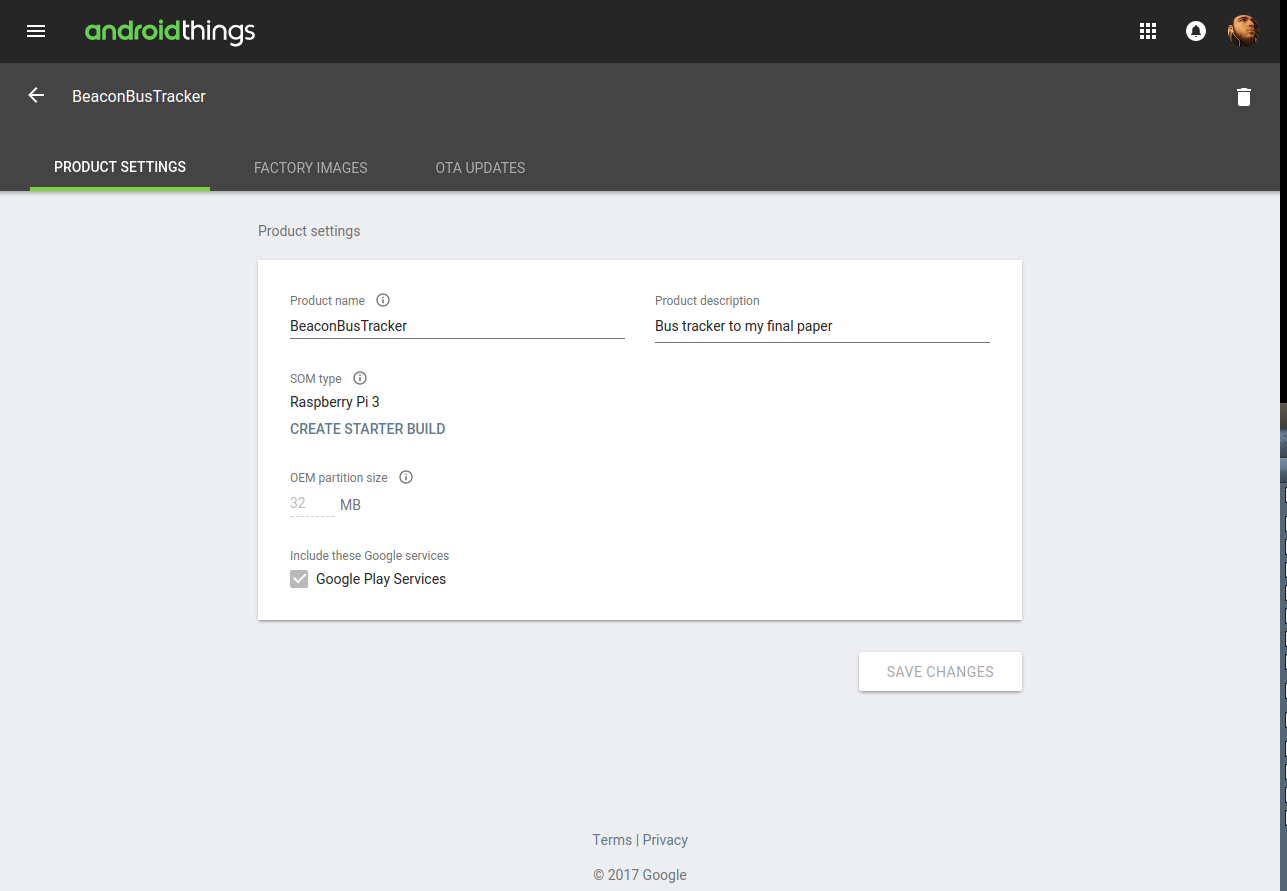
\includegraphics[width=15cm, center]{images/android-things-console-settings}
\caption{Página de configurações do produto criado.}
\label{Rotulo}
\end{figure}

\textbf{LocationManager}

O LocationManager é um serviço nativo que observa constantemente os dados de geolocalização do dispositivo. Com ele é possível ser notificado sobre as mudanças da posição, podendo configurar ser notificado quando se entra em determinada região, a cada tempo determinado ou quando se move por uma distância pré-definida. 

Este serviço abstrai toda lógica de acesso ao hardware e interpretação dos dados. Neste trabalho foi configurado para que ele notifique a geolocalização a cada 10 segundos.

\textbf{Peripheral Driver Library}

Não disponível na versão \textit{Android} para \textit{smartphones}, esta biblioteca oferece suporte ao \textit{Android Things} para que possa adicionar sensores e atuadores a placa utilizada, neste caso o \textit{Raspberry Pi 3}. Neste trabalho foi utilizado o \textit{Driver GPS} desta biblioteca para poder configurar o módulo \textit{NEO 6M}. O que possibilita o \textit{LocationManager} obter os dados de geolocalização, já que não existe sensor \textit{GPS} no \textit{Raspberry Pi 3}.

\subsubsection{IDE}

Foi escolhido o Android Studio como IDE do projeto. Ela é desenvolvida pela IntelliJ e tida pelo Google como ferramenta oficial de desenvolvimento para aplicativos Android.

\subsubsection{Animações}

Um dos tópicos mais presentes sobre melhorar experiência do usuário em \textit{Smartphones}, são as animações. Elas deixam o uso mais fluído e agradável para o usuário. 

Como cita \citecustom{Lecheta2015}, "Animações dão um acabamento profissional ao aplicativo, e costumam enriquecer a experiência do usuário.". Um dos tópicos mais presentes sobre melhorar experiência do usuário em \textit{smartphones}, são as animações, pois deixam o uso mais fluído e agradável para o usuário.

O \textit{Android Things} provê uma \textit{API} para animações que herdou da versão do \textit{Android} de \textit{smartphones}. Ela foi utilizada para melhorar a experiência de uso dos motoristas com o módulo, porém, foi observado uma baixa qualidade nas animações. O que fez ter o efeito contrário, pois passa a impressão de ser um sistema de baixo desempenho.

\section{Aplicativo}

\subsection{IDE}

Foi escolhido o Android Studio como IDE do projeto. Ela é desenvolvida pela IntelliJ e descrita pelo Google como a ferramenta oficial de desenvolvimento para aplicativos Android.

\subsection{Áudio Descrição}

Uma das funcionalidades do aplicativo é descrição em áudio da tela que o usuário está. O \textit{TalkBack} fala para o usuário em qual componente ele está tocando, porém, não descreve em qual tela ele acabou de entrar. 

A implementação por áudio descrição foi simples com uso da API nativa \textit{TextToSpeech}, onde podemos passar textos personalizados e o serviço se encarrega de sintetizar a voz.

O uso de uma camada de DI (Injeção de Dependências) facilitou o processo de implementação, fazendo ela na camada de serviço e configurando a instanciação no padrão \textit{Singleton} para que todos que vão utilizar (nesse caso são os \textit{presenters}), apenas solicitem a instância sendo passada por construtor.

\subsection{Usabilidade}

É uma boa prática no desenvolvimento de softwares, sempre confirmar se o usuário tem certeza que deseja executar alguma alteração que possa ter algum impacto no sistema ou em alguma funcionalidade, normalmente lançando alertas para garantir que o usuário não clicou sem querer em algum determinado botão, por exemplo. 

Inicialmente foi pensado em usar um \textit{dialog}, um pequeno quadrado que surge acima de todos componentes da tela com uma mensagem, para que o usuário confirme a ação de adicionar um ônibus como favorito, na tela de confirmação de acompanhamento. Ao testar a aplicação funcionando com \textit{Talkback}, foi observado que o sistema descreve o botão com o seguinte texto: \textit{"Adicionar aos favoritos. Botão, para acionar toque duas vezes"}. Esse texto já faz o usuário se assegurar da sua ação, tornando a prática de lançar um outro alerta ser algo desnecessário, fazendo o usuário ter um trabalho a mais de deslizar o dedo pela tela para encontrar os botões de \textit{OK} e cancelar do \textit{dialog.}

Com base nessas observações, não foi implementado \textit{dialogs} de confirmação. Deixando a responsabilidade de afirmar as ações do usuário para o \textit{Talkback} fazer. Embora seja uma pequena ação, tem grande impacto na usabilidade no quesito facilidade de uso do aplicativo por parte do usuário final, que são os deficientes visuais.

Outro ponto observado durante os testes foi a rotação da tela. O sistema operacional Android permite que aplicativos implementem variações da tela de acordo com a orientação do dispositivo, retrato ou paisagem. Isso permite que o layout do aplicativo se adapte a nova disposição de espaço.

Pensando no usuário final, para saber onde está cada elemento, ele precisa deslizar o dedo pela tela para conhecer a localização de cada um. Se ao rotacionar o aparelho, a disposição dos elementos mudar, o usuário precisa verificar novamente onde está cada um.

Como este trabalho desenvolve um aplicativo com poucos elementos na tela para simplificar o uso por deficientes visuais, foi bloqueado a mudança de tela ao rotacionar o aparelho. Isso garante um melhor conforto ao usar o aplicativo.


\section{Web service}

\subsection{Provedor de servidor}

%Falar sobre a umbler
Para tornar a aplicação acessível ao público, torna-se necessário que o servidor fique disponível constantemente, mantendo a API sempre ativa. 

Foram pesquisados três provedores de servidores, analisando qual deles apresentava melhores condições para realização do \textit{deploy} da aplicação. Foram eles a GoDaddy (https://br.godaddy.com/), Umbler (https://www.umbler.com/) e LocaWeb (https://www.locaweb.com.br).

Primeiro fator, que fez o serviço da GoDaddy ser excluído da lista, foi a questão de período de teste. A GoDaddy possui um período nulo de teste do serviço. Já a Umbler e LocaWeb fornecem créditos para novos desenvolvedores.

Em seguida, foi observada a disponibilidade de informações sobre como realizar o \textit{deploy} de um servidor em Node.js. Nesse aspecto, a LocaWeb não demonstra com clareza os procedimentos a serem seguidos.

A Umbler acabou sendo selecionada por ser muito intuitiva na hora de selecionar a linguagem da aplicação e qual o banco de dados a ser utilizado, com poucos cliques é possível iniciar um servidor funcional.


\subsection{Arquitetura}

Devido o uso do Express.js como intermediário para carregar os \textit{middlewares}, a arquitetura utilizada para o desenvolvimento da aplicação segue o padrão MVC.

\begin{figure}[H]
\centering
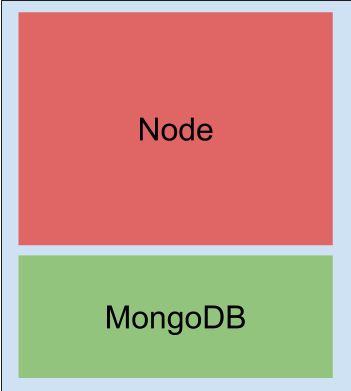
\includegraphics[width=5cm, center]{images/brick_diagram_framework_webservice}
\caption{Diagrama de blocos do Web Service.}
\label{Rotulo}
\end{figure}

\begin{description}
\item[Node] Cuida da parte de escalabilidade e conexão do servidor com os usuários da aplicação.
\item[MongoDB] Representa o banco de dados da aplicação, com as \textit{collections} necessárias para o funcionamento da aplicação.
\end{description}

O Node está subdividido da seguinte forma:

\begin{figure}[H]
\centering
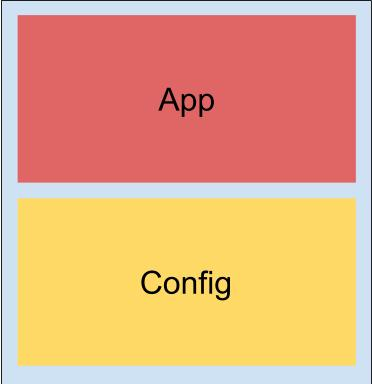
\includegraphics[width=5cm, center]{images/brick_diagram_node}
\caption{Diagrama de blocos do Node.}
\label{Rotulo}
\end{figure}

\begin{description}
\item[App] Conjunto com todas as funções da aplicação.
\item[Config] Possui os arquivos necessários para realizar as conexões com o servidor, banco de dados e o sistema de notificações.
\end{description}

Dentro do app é onde se observa a utilização da arquitetura MVC, ilustrada na Figura \ref{nodeapp}, representada da seguinte forma:

\begin{figure}[H]
\centering
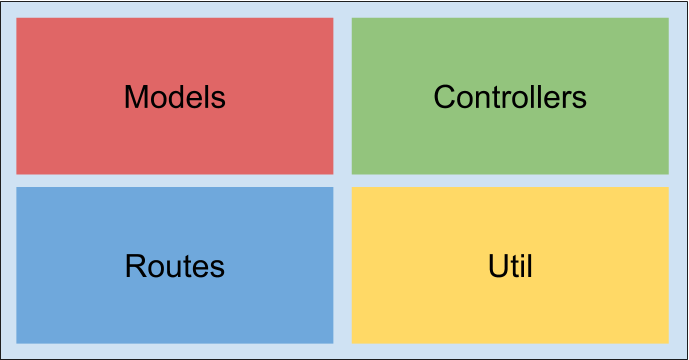
\includegraphics[width=10cm, center]{images/brick_diagram_node_app}
\caption{Diagrama de blocos do diretório app.}
\label{nodeapp}
\end{figure}

\begin{description}
\item[Models] Possui as regras de negócio da aplicação, com as informações necessárias para a criação das \textit{collections} do MongoDB através do mongoose e os arquivos com as funções de previsão de tempo e de correção de posição.
\item[Controllers] Possui as funções que utilizam os dados do banco de dados para gerar as informações adequadas aos usuários.
\item[Routes] Possui os arquivos com as rotas dos \textit{endpoints}, indicando qual arquivo e função dos \textit{controllers} será utilizado para a operação necessária pelo usuário, seguindo o padrão REST.
\item[Util] Possui as fórmulas necessárias para o desenvolvimento de certas funções da aplicação. 
\end{description}

\subsection{Localização do ônibus}

Ter conhecimento da posição do ônibus se faz necessário para realizar a previsão de chegada em um ponto de parada. Neste trabalho, sempre que o \textit{Web Service} recebe as coordenadas geográficas do ônibus, elas são corrigidas para um ponto válido da rota que este está fazendo.

Quando o \textit{Web Service} recupera as informações da rota do veículo, ele obtém todos os pontos referentes a ela, onde cada um tem informações de latitude, longitude e se este é um ponto de parada. Então é verificado qual ponto está mais próximo a localização recebida, o mais próximo é associado ao ônibus.

O cálculo de distância é feito a partir da fórmula \textit{Haversine}, encontrado em \citecustom{movablescripts}.

\begin{center}

$ a = \sin^2(\Delta\phi) + \cos\phi1 * \cos\phi2 * \sin^2(\Delta\lambda) $  \\
$ c = 2 * \atantwo(\sqrt{a},\sqrt{1 - a}) $ \\
$ d = R * c $ 

\end{center}

Onde: $ \Delta\phi = (latitude2 - latitude1), \phi1 = latitude1, \phi2 = latitude2, \Delta\lambda = longitude1 - longitude2 $ 

Foi observado que seria gasto muito processamento nessa parte. Uma tentativa de diminuir isso, foi o uso de um algoritmo de busca binária.

\textbf{Busca Binária}

\begin{flushright}
\textit{"Binary search is to algorithms
what a wheel is to mechanics:
It is simple, elegant, and immensely important."}
— Udi Manber, Introduction to Algorithms
\end{flushright}

Para otimizar a busca pelo ponto mais apto, foi estudado a busca binária. Ela segue o paradigma de dividir para conquistar. Tendo como premissa um \textit{array} de dados ordenados, primeiro observa os extremos do array, para em seguida observar o ponto médio entre eles. Caso um desses pontos seja igual ao valor procurado, assume ele como solução. Caso contrário se observa qual sub \textit{array} é mais apto, início até o centro ou do centro até o fim. O mais apto é submetido a uma nova busca binária. 

A vantagem em se utilizar uma busca binária ao invés de uma busca sequencial pode ser observado pelas suas complexidades. A busca binária possui complexidade $O(\log_2 n)$, enquanto a sequencial possui complexidade $O(n)$

A tabela a seguir mostra o número de vezes que cada busca iria precisar fazer para chegar no ponto mais apto.

\begin{tabular}{|c|c|c|c|}
\hline 
Rota & Número de Pontos & Busca Binária $(O(\log_2 n)$) & Busca Sequencial ($O(n)$) \\ 
\hline 
1 & 410 & \simeq 9 & 410 \\ 
\hline 
2 & 500 & \simeq 9 & 500 \\ 
\hline 
3 & 675 & \simeq 10 & 675 \\ 
\hline 
4 & 708 & \simeq 10 & 708 \\ 
\hline 
5 & 725 & \simeq 10 & 725 \\ 
\hline 
\end{tabular} 
\\

A implementação da busca ficou da seguinte forma:

Primeiro é calculado a distância entre a localização recebida do ônibus e o primeiro ponto da rota. 
Em seguida, calculamos a distância entre a localização recebida e o último ponto da rota. Com isso temos a distânciaInicio e distânciaFim. 

\begin{figure}[H]
\centering
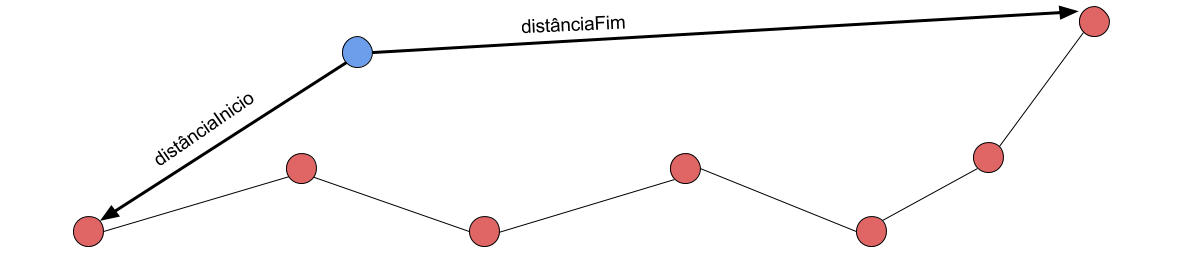
\includegraphics[width=12cm, center]{images/distanciainicio-distanciafim.png}
\caption{Representação da busca binária I.}
\label{Rotulo}
\end{figure}

Um terceiro cálculo é feito, a distância entre a localização recebida e o ponto do meio da rota.

\begin{figure}[H]
\centering
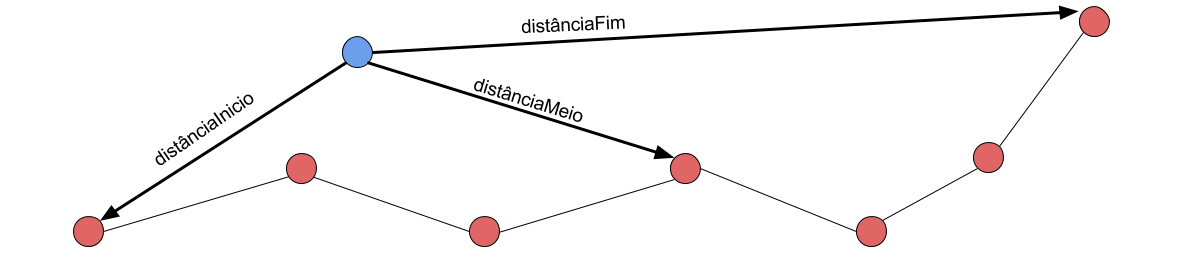
\includegraphics[width=12cm, center]{images/distanciainicio-distanciafim-distanciomeio.png}
\caption{Representação da busca binária II.}
\label{Rotulo}
\end{figure}

O algoritmo então verifica qual metade é mais apta, baseando-se nas distâncias mais curtas. Se distânciaFim é maior que distânciaInicio, é feito uma recursividade assumindo distânciaMeio como fim.

\begin{figure}[H]
\centering
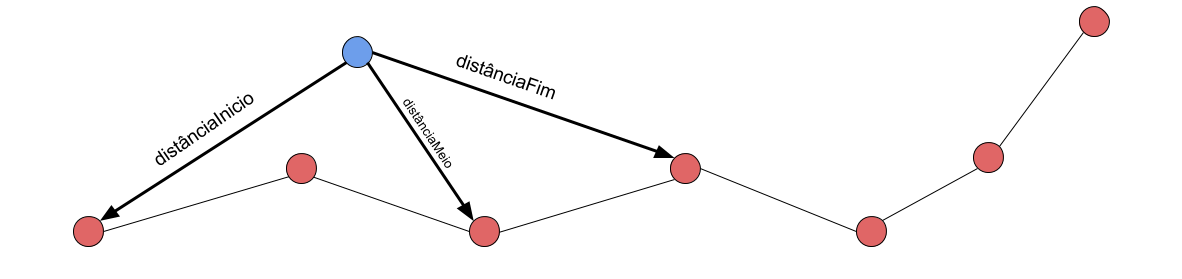
\includegraphics[width=12cm, center]{images/nova-distancia.png}
\caption{Representação da busca binária III.}
\label{Rotulo}
\end{figure}

Fazendo isso sucessivamente, chega uma hora que não é mais possível dividir, então o ponto mais próximo assume o posto de mais apto e é associado ao ônibus.

\textbf{Resultados}

Após realizar testes foi comprovado que embora exista a melhora em diminuir drasticamente o processamento, foi encontrado o problema do ponto correto estar em um sub \textit{array} que não é considerado o mais apto, como ilustra a Figura \ref{binary-search-problem}.

\begin{figure}[H]
\centering
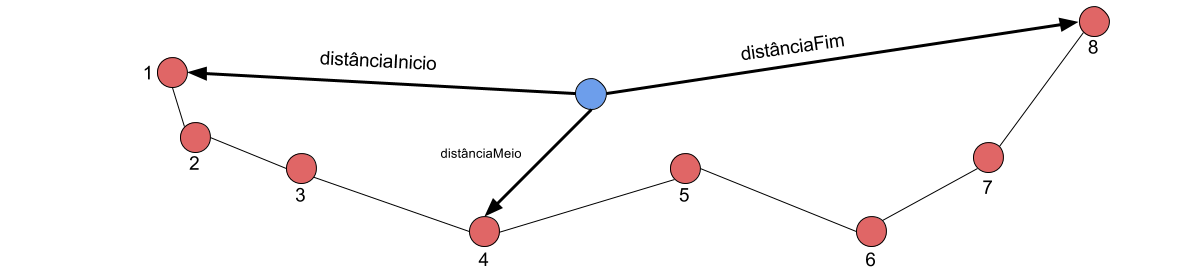
\includegraphics[width=12cm, center]{images/busca-binaria-problema}
\caption{Representação do problema da busca binária.}
\label{binary-search-problem}
\end{figure}

Como pode se observar na Figura \ref{binary-search-problem}, o ponto mais próximo em relação a posição recebida é o número 5. Quando se inicia a busca binária, o ponto número 4 é considerado o centro, tornando o sub \textit{array} distânciaInicio até distânciaMeio ser o mais apto para se realizar uma busca interna, fazendo o ponto número 5 ser desconsiderado.

Embora a busca binária demonstre ser mais eficiente que a busca sequencial, a implementação neste problema, tendo como heurística a menor distância, demonstrou não ser suficiente para diminuir o processamento e encontrar a melhor solução.

\subsection{Previsão de chegada}

Para calcular a previsão de chegada de um ônibus, é necessário saber a última localização conhecida dele e o ponto de parada escolhido. Com essas duas informações pode-se recuperar todos dados necessários para o cálculo.

\begin{figure}[H]
\centering
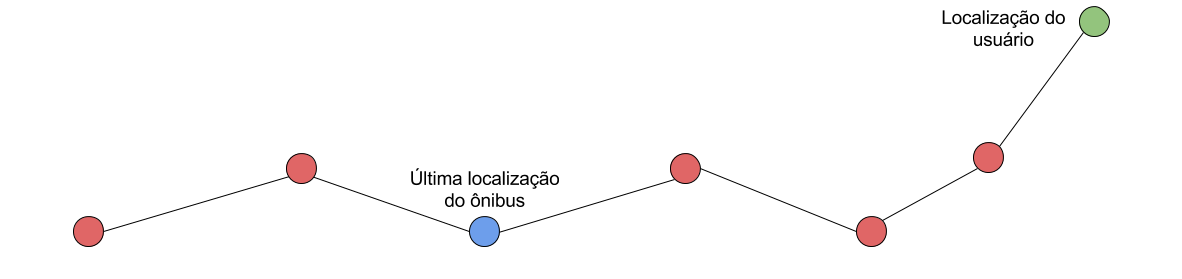
\includegraphics[width=15cm, center]{images/previsao-rota}
\caption{Representação de uma rota.}
\label{Rotulo}
\end{figure}

Primeiro é recuperado todos os dados da rota que o ônibus está fazendo. Cada rota possui N pontos associados a ela, onde cada um tem a informação de latitude, longitude e se este é um ponto de parada. Sabendo em qual ponto da rota o ônibus está e qual ponto de parada o usuário se encontra, podemos pegar todos os pontos que estão entre eles e calcular a distância com a seguinte fórmula.

\begin{center}
$t = \dfrac{s}{v}$ 
\end{center}

A partir disso se soma a distância dentre todos esses pontos, a partir do resultado se divide pela velocidade da pista e se obtém quanto tempo aproximado falta para o ônibus chegar na parada.

\subsection{Alertar motorista sobre parar}

O \textit{Android Things} não suporta serviço de \textit{push notification}. Para enviar mensagens instantâneas ao módulo foi utilizado o \textit{Realtime Database}, do \textit{Firebase}, que permite observar um nó. Sempre que existe uma alteração deste, quem está observando é notificado.

\begin{figure}[H]
\centering
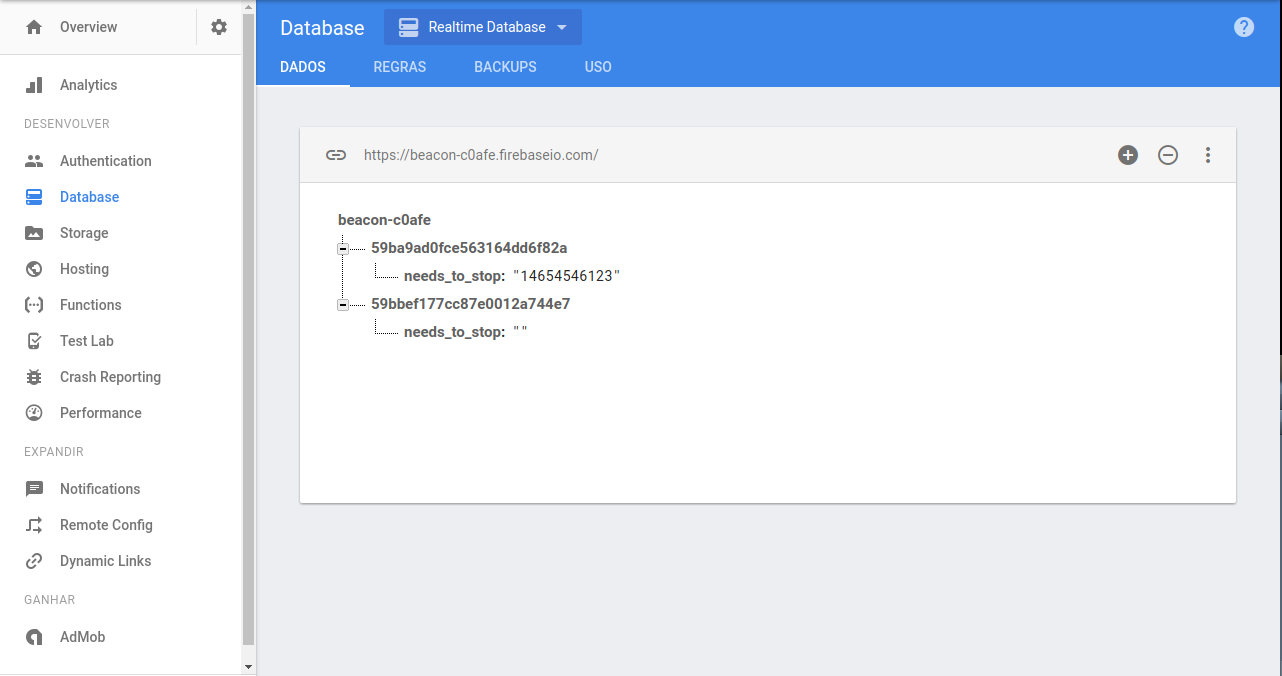
\includegraphics[width=15cm, center]{images/realtime-database}
\caption{Painel de controle do Firebase Realtime Database.}
\label{Rotulo}
\end{figure}

Quando um módulo do ônibus é conectado a internet, ele cria um nó com seu ID na base de dados e um nó filho intitulado \textit{needs\_to\_stop}, e passa a observá-lo. Quando o valor do nó filho é alterado, o módulo então dispara uma notificação para o motorista sobre a necessidade de parar no próximo ponto de ônibus.

O responsável por alterar o valor do nó filho é o \textit{Web Service}. Como visto na seção \textit{Localização do Ônibus}, é feito uma varredura para descobrir o ponto da rota que o ônibus se encontra. Em seguida também é verificado qual o próximo ponto que ele vai passar. Caso o próximo ponto esteja na lista de requisições de parada, é então alterado o valor do nó filho para que aquele módulo alerte o motorista.

\subsection{Alertar usuário que ônibus chegou}

Quando o motorista chega na parada, ele pressiona um botão para anunciar sua chegada. Quando \textit{Web Service} recebe esse alerta por meio de uma requisição \textit{HTTP}, ele verifica quais usuários estão aguardando aquele ônibus, então é disparado uma \textit{push notification}, por meio do \textit{Firebase}, avisando que o ônibus que ele aguarda está parado.

\chapter{Considerações Finais}

Com os avanços tecnológicos, surgem diversas ferramentas que facilitam a vida de seus usuários. Porém, nem sempre essas ferramentas alcançam a todos, sendo de difícil manuseio para determinados grupos, como, por exemplo, o dos deficientes visuais. Os aplicativos de monitoramento de transportes públicos, que indicam uma previsão de quanto tempo até que o ônibus chegue na parada em que o usuário se encontra é um desses casos. Começando com o fato de ser necessário que o usuário ajuste manualmente a sua posição inicial num mapa de modo a melhorar a precisão de sua localização. Esse passo dificulta muito a utilização do aplicativo para um usuário deficiente visual. Mesmo os aplicativos que possuem uma integração com algum tipo de tecnologia assistiva, como o Talkback da Google, acabam possuindo alguma dificuldade de uso.

Neste trabalho foi possível desenvolver um aplicativo nativo em Android, adaptado com o Talkback e com feedback descritivo das telas por meio de áudio, uma aplicação Web implementando a API do sistema, além dos protótipos dos módulos do ponto de ônibus e dos ônibus. O módulo do ponto envia um sinal constante com o ID do ponto, com isso, o aplicativo pede para a aplicação Web uma lista com os ônibus que estão em circulação e que passam por aquele ponto, além de obter uma previsão para sua chegada. Após o usuário confirmar qual ônibus ele deseja esperar, é criada uma requisição que analisa as informações, alimentadas pelo módulo do ônibus, para disparar um aviso ao módulo do ônibus dizendo que é preciso parar na próxima parada por existir um deficiente visual esperando-o. O sistema se comportou como esperado, provendo facilidades de uso na hora de escolher o ônibus, demonstrando ser uma boa solução para facilitar o uso deste transporte público.

O objetivo principal deste trabalho foi desenvolver uma solução para facilitar a forma como deficientes visuais utilizam os ônibus, sem o foco de elaborar um sistema de previsão de horários mais preciso. Isso gerou a possibilidade de diversos aprimoramentos futuros que podem ser adicionados a este sistema, como: alterar a linha quando termina uma rota; melhorar a tratativa de velocidade do ônibus para considerar velocidades médias de um trecho possibilitando uma previsão de chegada mais precisa; e a implementação de uma interface gráfica para controlar os registros que existem no banco de dados da aplicação Web, a fim de facilitar seu uso.

\postextual

\bibliography{beacon-final-paper}

\begin{apendicesenv}
\partapendices

\chapter{Diagrama de Classes}

\begin{figure}[H]
\centering
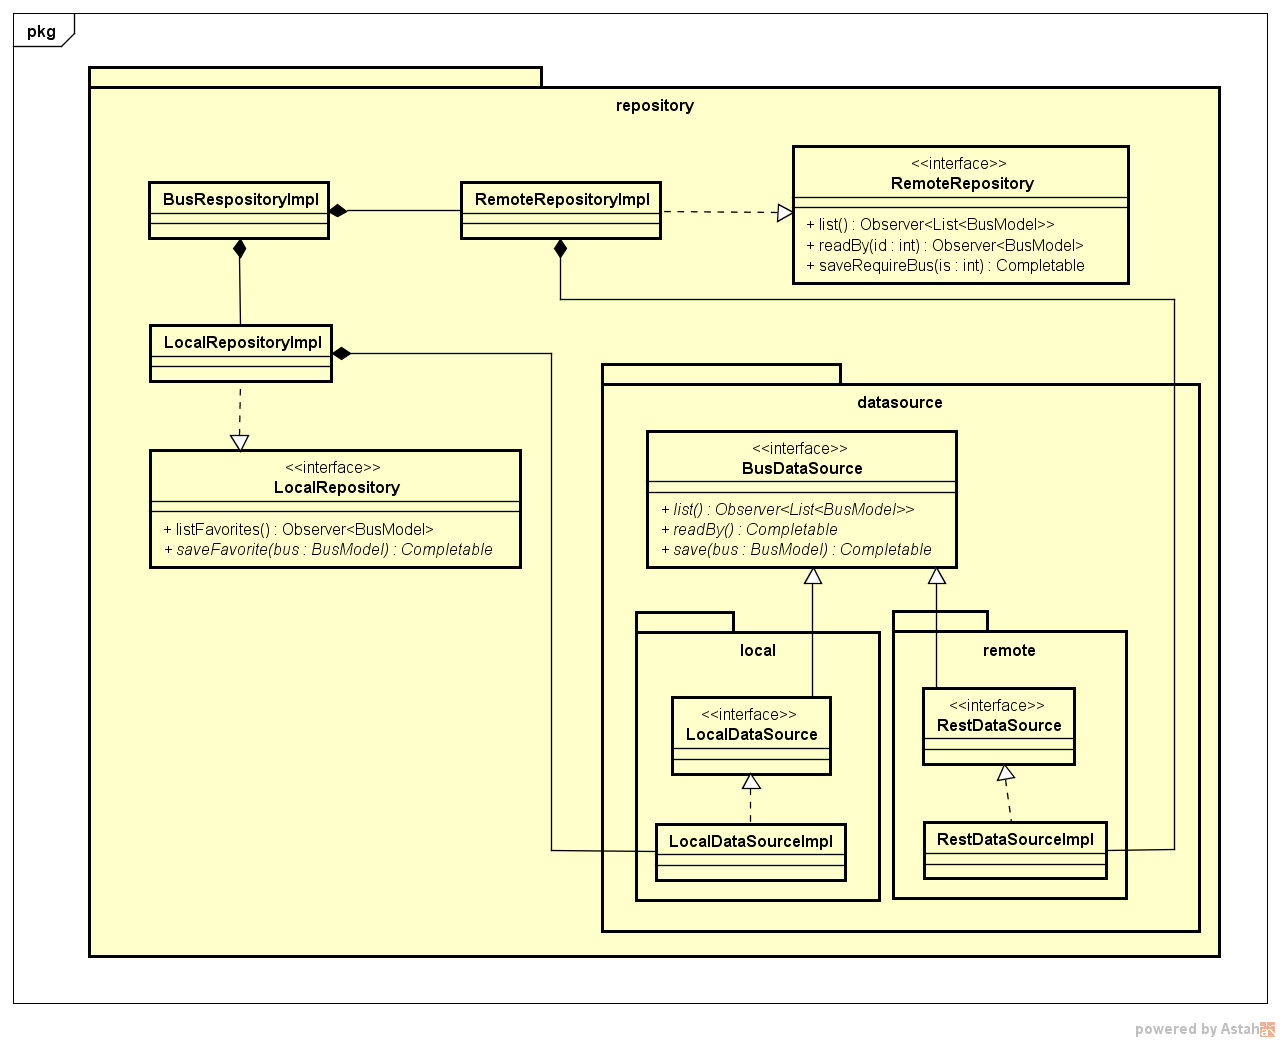
\includegraphics[width=15cm, center]{images/data-layer}
\caption{Diagrama de classes da camada de dados.}
\label{Rotulo}
\end{figure}

\begin{figure}[H]
\centering
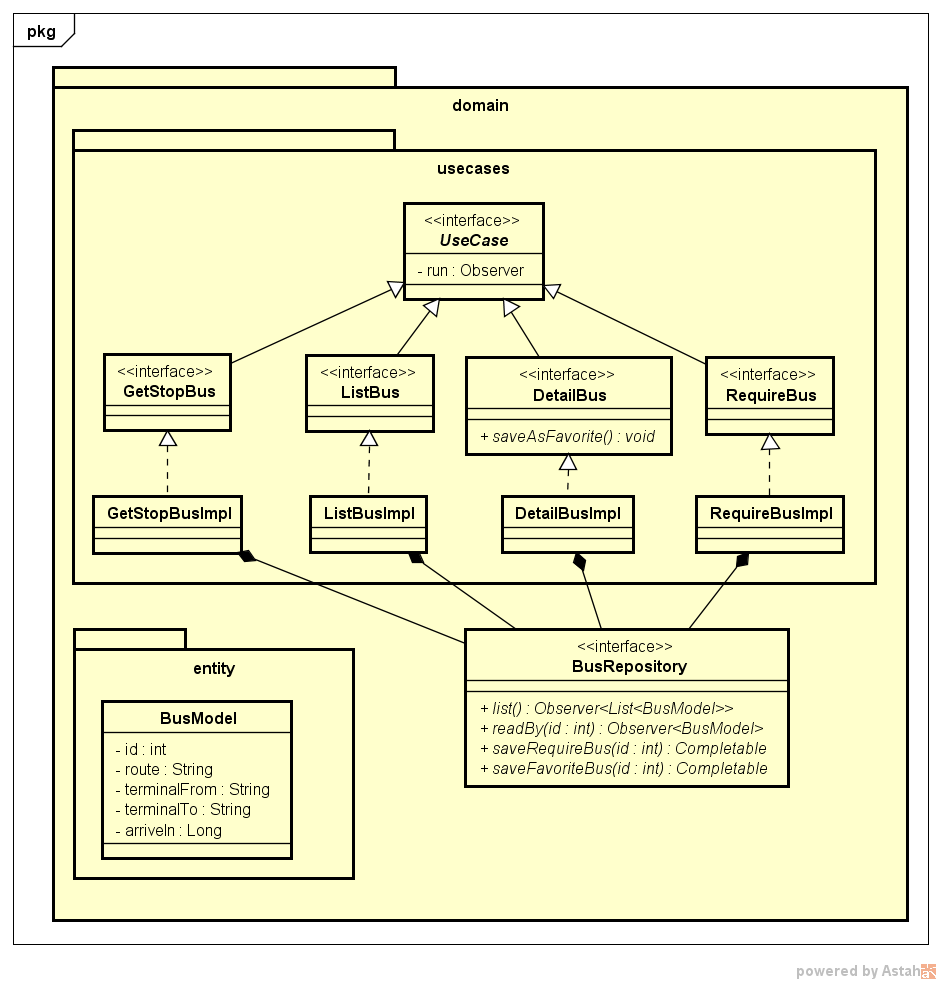
\includegraphics[width=15cm, center]{images/domain-layer}
\caption{Diagrama de classes da camada de domínio.}
\label{Rotulo}
\end{figure}

\begin{figure}[H]
\centering
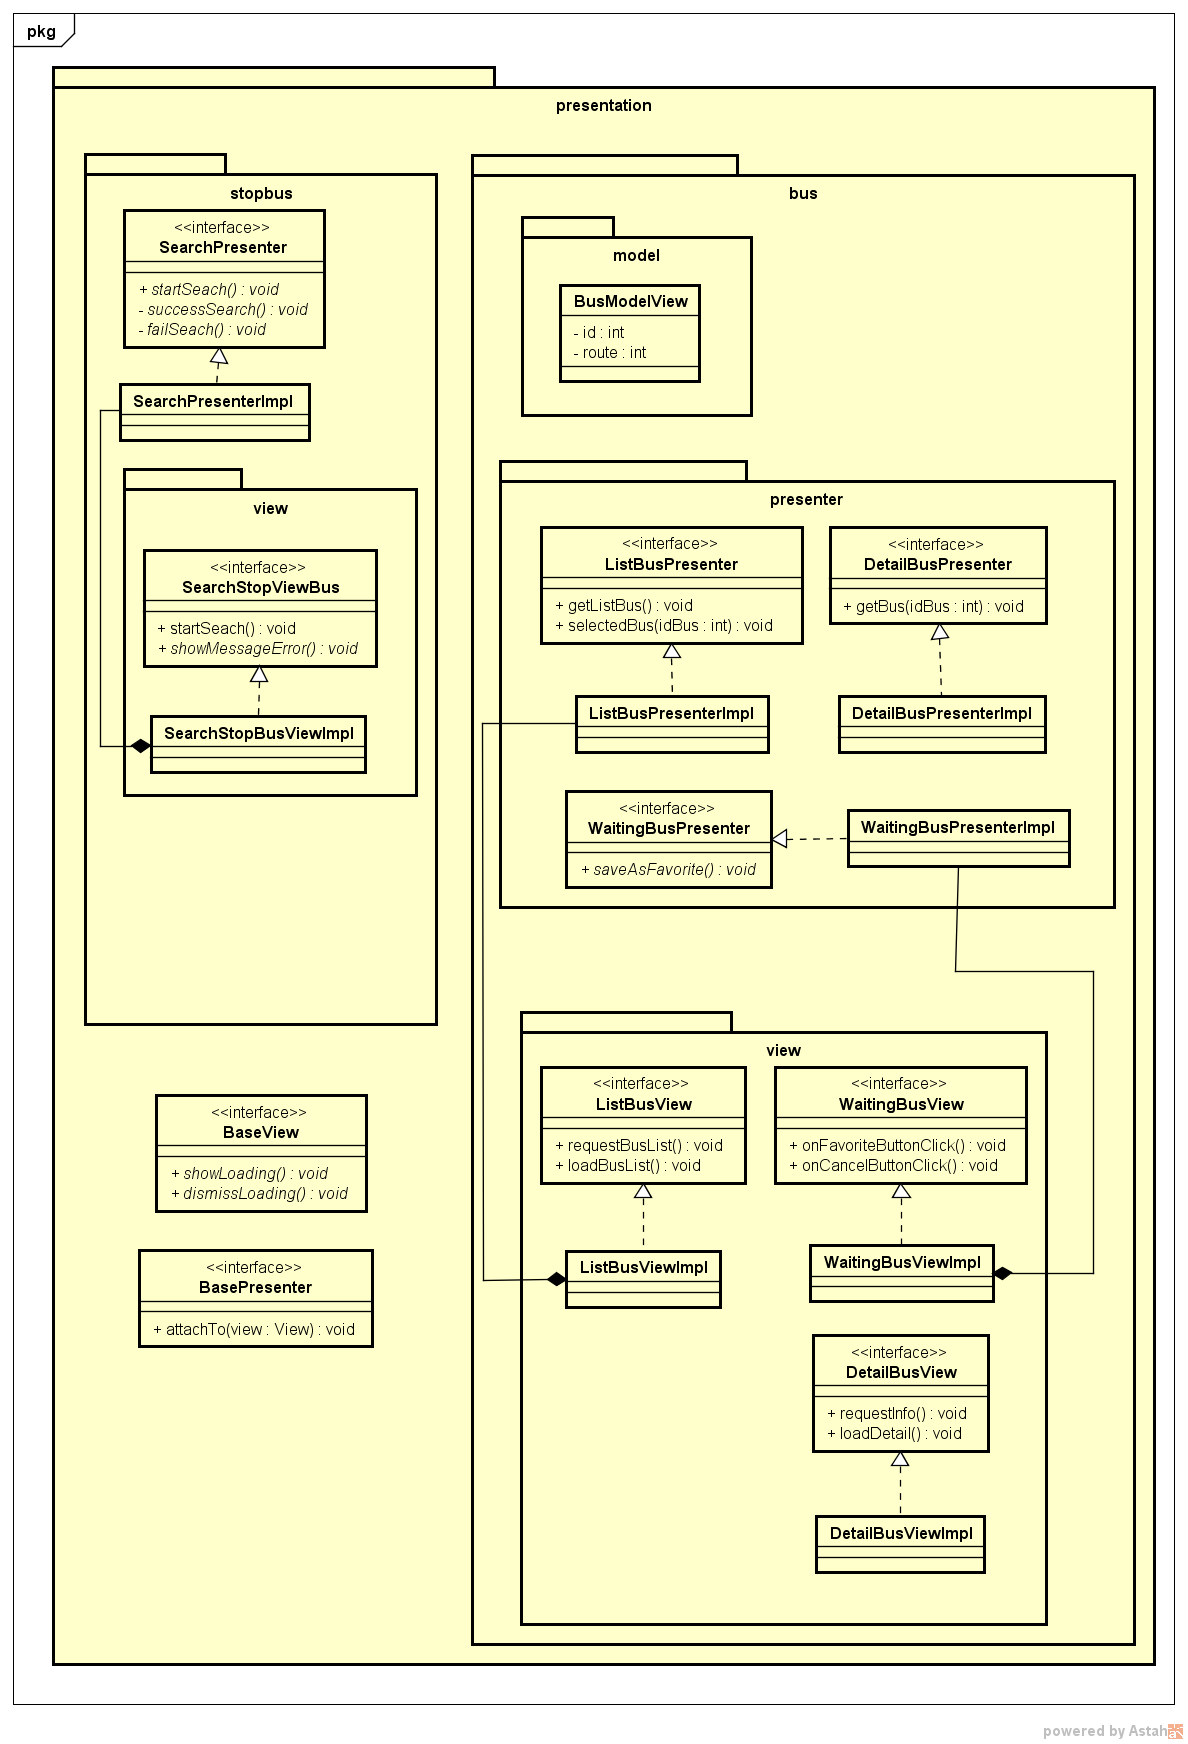
\includegraphics[width=15cm, center]{images/presentation-layer}
\caption{Diagrama de classes da camada de apresentação.}
\label{Rotulo}
\end{figure}

\chapter{Wireframes}

\begin{figure}[H]
\centering
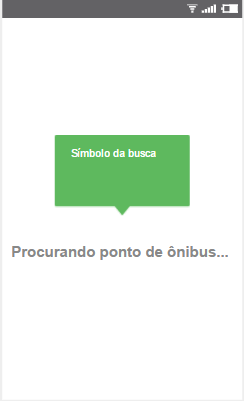
\includegraphics[width=5cm, center]{images/tela-1-buscando-beacon.PNG}
\caption{Wireframe da tela do aplicativo ao buscar por um ponto de ônibus próximo.}
\label{Rotulo}
\end{figure}

\begin{figure}[H]
\centering
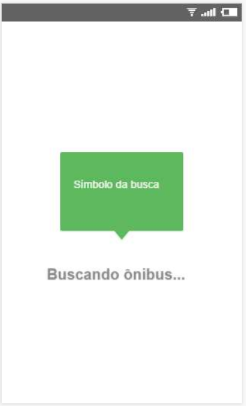
\includegraphics[width=5cm, center]{images/tela-2-buscando-ponto.PNG}
\caption{Wireframe da tela do aplicativo ao buscar por um ponto de ônibus na API.}
\label{Rotulo}
\end{figure}

\begin{figure}[H]
\centering
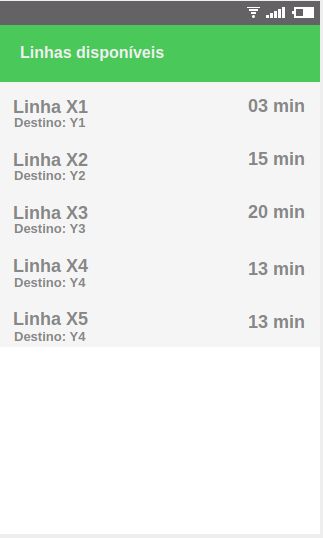
\includegraphics[width=5cm, center]{images/tela-3-lista-de-onibus.PNG}
\caption{Wireframe da tela do aplicativo com ônibus disponíveis.}
\label{Rotulo}
\end{figure}

\begin{figure}[H]
\centering
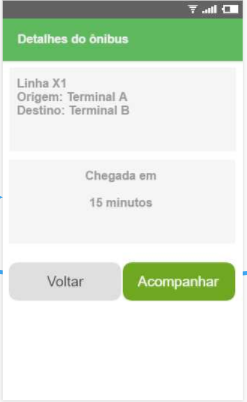
\includegraphics[width=5cm, center]{images/tela-4-informacoes-do-onibus.PNG}
\caption{Wireframe da tela do aplicativo com detalhes de um ônibus.}
\label{Rotulo}
\end{figure}

\begin{figure}[H]
\centering
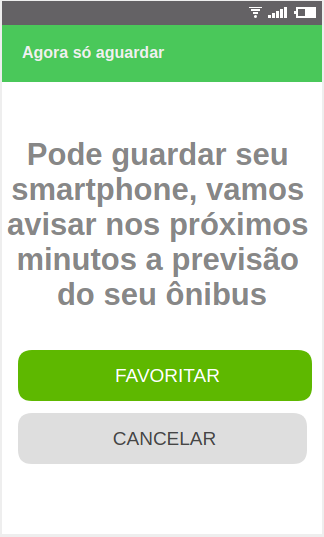
\includegraphics[width=5cm, center]{images/tela-5-acompanhamento-do-onibus.PNG}
\caption{Wireframe da tela do aplicativo sobre a solicitação de um ônibus.}
\label{Rotulo}
\end{figure}

\begin{figure}[H]
\centering
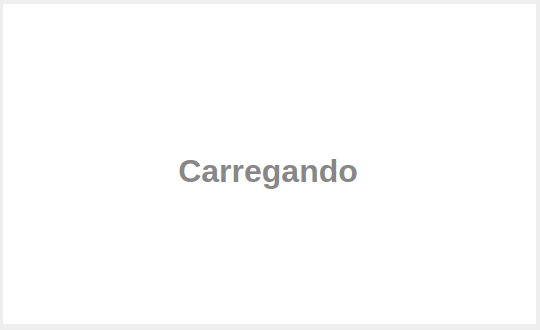
\includegraphics[width=10cm, center]{images/busmodule-carregando}
\caption{Wireframe da tela do módulo do ônibus quando está carregando informações.}
\label{Rotulo}
\end{figure}

\begin{figure}[H]
\centering
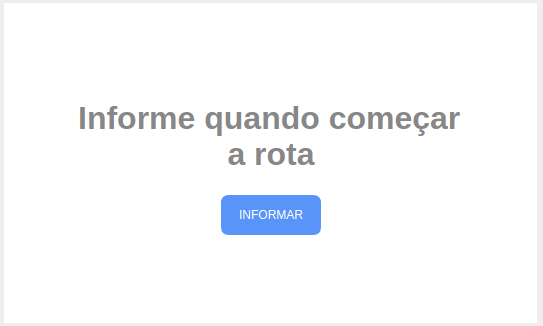
\includegraphics[width=10cm, center]{images/busmodule-comecar-rota}
\caption{Wireframe da tela do módulo do ônibus aguardando motorista iniciar rota.}
\label{Rotulo}
\end{figure}

\begin{figure}[H]
\centering
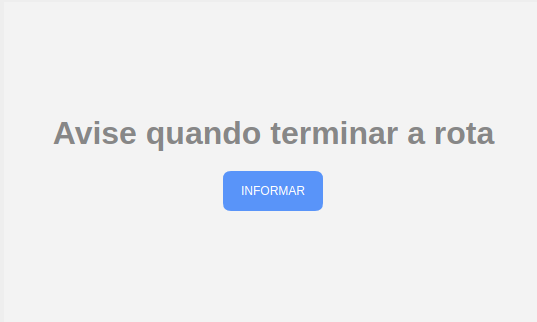
\includegraphics[width=10cm, center]{images/busmodule-finish-route}
\caption{Wireframe da tela do módulo do ônibus quando motorista está fazendo a rota.}
\label{Rotulo}
\end{figure}

\begin{figure}[H]
\centering
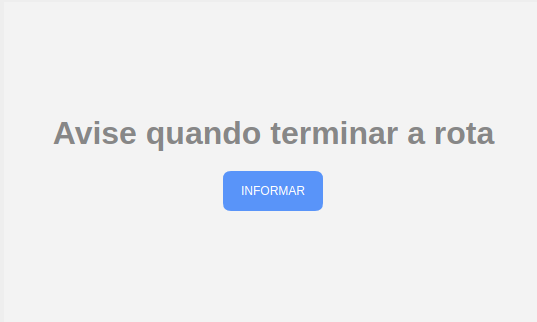
\includegraphics[width=10cm, center]{images/busmodule-finish-route}
\caption{Wireframe da tela do módulo do ônibus quando motorista está fazendo a rota.}
\label{Rotulo}
\end{figure}

\begin{figure}[H]
\centering
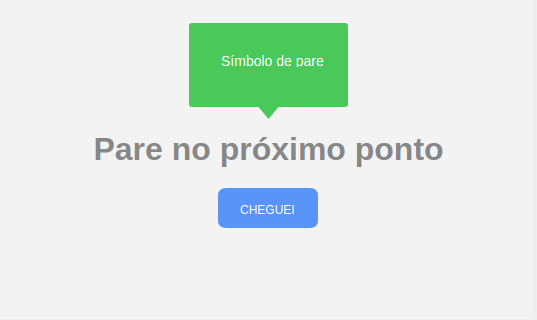
\includegraphics[width=10cm, center]{images/busmodule-pare}
\caption{Wireframe da tela do módulo do ônibus quando motorista precisar parar no próximo ponto.}
\label{Rotulo}
\end{figure}

\chapter{Testes de aceitação}

Os testes de aceitação visam fazer um conjunto de testes isolados uns dos outros para garantir a qualidade e as funcionalidades do aplicativo.

Cada teste está organizado na seguinte estrutura:

\bgroup
\def\arraystretch{1.5}
\begin{table}[H]

\begin{tabularx}{\textwidth}{|l|>{\hsize=2\hsize}X|c|}
\hline 
\textbf{ID:} x.x.x & \textbf{Título:}  & \textbf{Nível do teste} \\ 
\hline 
\multicolumn{3}{|>{\hsize=\dimexpr3\hsize+3\tabcolsep+\arrayrulewidth\relax}X|}{\textbf{Descrição:}} \\ 
\hline  
\multicolumn{3}{|>{\hsize=\dimexpr3\hsize+3\tabcolsep+\arrayrulewidth\relax}X|}{\textbf{Necessário para:}} \\ 
\hline 
\multicolumn{3}{|>{\hsize=\dimexpr3\hsize+3\tabcolsep+\arrayrulewidth\relax}X|}{\textbf{Nota de teste:}} \\ 
\hline 
\multicolumn{3}{|>{\hsize=\dimexpr3\hsize+3\tabcolsep+\arrayrulewidth\relax}X|}{\textbf{Etapas:}} \\ 
\hline 
\multicolumn{3}{|X|}{\textbf{Resultado:} Sucesso/Falha} \\ 
\hline 
\end{tabularx} 

\end{table}
\egroup

\begin{itemize}

\item \textbf{ID:} Identificador único para um teste.
\item \textbf{Título: }Texto breve que identifica o que será testado.
\item \textbf{Nível do teste:} Identifica se o teste é crítico para o sistema.
\item \textbf{Descrição:} Texto explicando com mais detalhes o que será testado.
\item \textbf{Necessário para:} Cliente que fará uso da funcionalidade.
\item \textbf{Nota de teste:} Observações a serem feitas antes de realizar o teste.
\item \textbf{Etapas:} Passo a passo para reprodução do teste.
\item \textbf{Resultado:} Apresenta o resultado do teste realizado.

\end{itemize}

\newpage

\subsection*{Nível de teste}

Os sistemas possuem diversas funcionalidades e pré-requisitos para funcionar corretamente. Cada uma tem seu grau de importância para o sistema, que dependendo deste grau, pode afetar totalmente ou parcialmente seu uso caso esteja com algum problema na implementação. Por isso, é de extrema importância identificar o quanto um teste pode impactar no sistema, para quando falhar, gerar um alerta de mau funcionamento.

Os níveis dos testes, indicados no canto superior direito da tabela de cada teste, servem para alertar o quão importante o teste significa para o correto funcionamento do sistema que a funcionalidade pertence, podendo apresentar dois níveis: “Crítico” ou “Atenção”.

Crítico: Representa uma funcionalidade de extrema importância para o correto funcionamento do sistema. Caso este teste falhe, o sistema não terá o comportamento necessário para funcionar como o usuário deseja. Sua indicação apresenta um fundo vermelho. 

Atenção: Representa uma funcionalidade importante para o sistema. Caso o teste falhe, não afetará o funcionamento do sistema. Pode impactar em performance ou usabilidade reduzida, mas não em valores entregues ao usuário. Sua indicação apresenta um fundo azul.

\newpage

\subsection*{Módulo do ponto de ônibus (\textit{Beacon})}

\subsubsection*{Emissão de sinal}

\bgroup
\def\arraystretch{1.5}

\begin{table}[H]

\begin{tabularx}{\textwidth}{|l|>{\hsize=2\hsize}X|c|}
\hline 
\textbf{ID:} 1.1.1 & \textbf{Título:} Emissão de ID único
 & \textbf{Crítico} \\ 
\hline 
\multicolumn{3}{|>{\hsize=\dimexpr3\hsize+3\tabcolsep+\arrayrulewidth\relax}X|}{\textbf{Descrição:} Este teste irá verificar se o módulo está emitindo um sinal com id único de acordo com padrões estabelecidos.
} \\ 
\hline  
\multicolumn{3}{|>{\hsize=\dimexpr3\hsize+3\tabcolsep+\arrayrulewidth\relax}X|}{\textbf{Necessário para:} Aplicativo} \\ 
\hline 
\multicolumn{3}{|>{\hsize=\dimexpr3\hsize+3\tabcolsep+\arrayrulewidth\relax}X|}{\textbf{Nota de teste:} O sinal emitido é de acordo com a tecnologia \textit{Bluetooth BLE} (4.+).
O canal utilizado para a emissão do ID é o “id1” de acordo com as especificações dos \textit{Beacons}.
O padrão estabelecido para o ID emitido é 655xxxx, sendo ‘x’ qualquer valor do conjunto dos números Naturais.
} \\ 
\hline 
\multicolumn{3}{|>{\hsize=3\hsize}X|}{\textbf{Etapas:} 


1. Ativar o módulo 


2. Receber o sinal


3. Verificar se o canal "id1" está de acordo com o padrão
} \\ 
\hline 
\multicolumn{3}{|X|}{\textbf{Resultado:} } \\ 
\hline 
\end{tabularx} 

\end{table}

\egroup

\newpage

\subsection*{Módulo do ônibus}

\subsubsection*{Geolocalização}

\bgroup
\def\arraystretch{1.5}
\begin{table}[H]

\begin{tabularx}{\textwidth}{|l|>{\hsize=2\hsize}X|c|}
\hline 
\textbf{ID:} 2.1.1 & \textbf{Título:} Emissão de geolocalização & \textbf{Crítico} \\ 
\hline 
\multicolumn{3}{|>{\hsize=\dimexpr3\hsize+3\tabcolsep+\arrayrulewidth\relax}X|}{\textbf{Descrição:} Este teste irá verificar se o módulo está enviando a geolocalização do veículo
} \\ 
\hline  
\multicolumn{3}{|>{\hsize=\dimexpr3\hsize+3\tabcolsep+\arrayrulewidth\relax}X|}{\textbf{Necessário para:} \textit{Web service}} \\ 
\hline 
\multicolumn{3}{|>{\hsize=\dimexpr3\hsize+3\tabcolsep+\arrayrulewidth\relax}X|}{\textbf{Nota de teste:} O envio dos dados deve estar de acordo com a notação JSON. Deve ser enviado em determinados intervalos de tempo, conforme definido no \textit{web service}.} \\ 
\hline 
\multicolumn{3}{|>{\hsize=\dimexpr3\hsize+3\tabcolsep+\arrayrulewidth\relax}X|}{\textbf{Etapas:}

1. Ativar o módulo

2. Verificar se o \textit{Web Service} está recebendo a geolocalização

3. Verificar se os dados recebidos estão chegando de acordo com o tempo definido
} \\ 
\hline 
\multicolumn{3}{|X|}{\textbf{Resultado:} } \\ 
\hline 
\end{tabularx} 
\end{table}
\egroup

\subsubsection*{Interação com motorista}

\bgroup
\def\arraystretch{1.5}
\begin{table}[H]

\begin{tabularx}{\textwidth}{|l|>{\hsize=2\hsize}X|c|}
\hline 
\textbf{ID:} 2.2.1 & \textbf{Título:} Emissão de alerta de parada & \textbf{Crítico} \\ 
\hline 
\multicolumn{3}{|>{\hsize=\dimexpr3\hsize+3\tabcolsep+\arrayrulewidth\relax}X|}{\textbf{Descrição:} Este teste irá verificar se o módulo está recebendo notificações de alerta e notificando ao motorista sobre a necessidade de parada no próximo ponto} \\ 
\hline  
\multicolumn{3}{|>{\hsize=\dimexpr3\hsize+3\tabcolsep+\arrayrulewidth\relax}X|}{\textbf{Necessário para:} Módulo de ônibus} \\ 
\hline 
\multicolumn{3}{|>{\hsize=\dimexpr3\hsize+3\tabcolsep+\arrayrulewidth\relax}X|}{\textbf{Nota de teste:} O envio do alerta se faz por meio do serviço do \textit{Firebase Realtime Database}.} \\ 
\hline 
\multicolumn{3}{|>{\hsize=\dimexpr3\hsize+3\tabcolsep+\arrayrulewidth\relax}X|}{\textbf{Etapas:}

1. Ativar o módulo

2. Alterar a variável no \textit{Firebase Realtime Database} de alerta de parada

3. Verificar se houve a emissão do alerta de parada
} \\ 
\hline 
\multicolumn{3}{|X|}{\textbf{Resultado:}} \\ 
\hline 
\end{tabularx} 
\end{table}
\egroup

\subsection*{Aplicativo Mobile}

\subsubsection*{Instalação}

\bgroup
\def\arraystretch{1.5}
\begin{table}[H]

\begin{tabularx}{\textwidth}{|l|>{\hsize=2\hsize}X|c|}
\hline 
\textbf{ID:} 3.1.1 & \textbf{Título:} Instalação realizada com sucesso
 & \textbf{Crítico} \\ 
\hline 
\multicolumn{3}{|>{\hsize=\dimexpr3\hsize+3\tabcolsep+\arrayrulewidth\relax}X|}{\textbf{Descrição:} Este teste irá verificar se o aplicativo foi instalado com sucesso} \\ 
\hline  
\multicolumn{3}{|>{\hsize=\dimexpr3\hsize+3\tabcolsep+\arrayrulewidth\relax}X|}{\textbf{Necessário para:}} \\ 
\hline 
\multicolumn{3}{|>{\hsize=\dimexpr3\hsize+3\tabcolsep+\arrayrulewidth\relax}X|}{\textbf{Nota de teste:}  A versão do Android instalada deve ser no mínimo a versão Jelly Beans (v4.1).
} \\ 
\hline 
\multicolumn{3}{|>{\hsize=\dimexpr3\hsize+3\tabcolsep+\arrayrulewidth\relax}X|}{\textbf{Etapas:}

1. Instale a aplicação no dispositivo

2. Navegue até a lista de aplicativos

3. Verifique se o aplicativo \textit{Beacon} está listado.
} \\ 
\hline 
\multicolumn{3}{|X|}{\textbf{Resultado:}} \\ 
\hline 
\end{tabularx} 
\end{table}
\egroup

\bgroup
\def\arraystretch{1.5}
\begin{table}[H]

\begin{tabularx}{\textwidth}{|l|>{\hsize=2\hsize}X|c|}
\hline 
\textbf{ID:} 3.1.2 & \textbf{Título:} Talkback ativo & \textbf{Atenção} \\ 
\hline 
\multicolumn{3}{|>{\hsize=\dimexpr3\hsize+3\tabcolsep+\arrayrulewidth\relax}X|}{\textbf{Descrição:} Este teste irá verificar se o talkback está ativo} \\ 
\hline  
\multicolumn{3}{|>{\hsize=\dimexpr3\hsize+3\tabcolsep+\arrayrulewidth\relax}X|}{\textbf{Necessário para:}} \\ 
\hline 
\multicolumn{3}{|>{\hsize=\dimexpr3\hsize+3\tabcolsep+\arrayrulewidth\relax}X|}{\textbf{Nota de teste:}} \\ 
\hline 
\multicolumn{3}{|>{\hsize=\dimexpr3\hsize+3\tabcolsep+\arrayrulewidth\relax}X|}{\textbf{Etapas:}

1. Navegue pela tela passando pelos ícones disponíveis

2. Verifique se está sendo emitido a áudio descrição dos ícones.
} \\ 
\hline 
\multicolumn{3}{|X|}{\textbf{Resultado:}} \\ 
\hline 
\end{tabularx} 
\end{table}
\egroup

\subsubsection*{Tela}

\bgroup
\def\arraystretch{1.5}
\begin{table}[H]

\begin{tabularx}{\textwidth}{|l|>{\hsize=2\hsize}X|c|}
\hline 
\textbf{ID:} 3.2.1 & \textbf{Título:}  Áudio descrições
 & \textbf{Atenção} \\ 
\hline 
\multicolumn{3}{|>{\hsize=\dimexpr3\hsize+3\tabcolsep+\arrayrulewidth\relax}X|}{\textbf{Descrição:}  Este teste irá verificar se o talkback está conseguindo ler os componentes da tela no aplicativo
} \\ 
\hline  
\multicolumn{3}{|>{\hsize=\dimexpr3\hsize+3\tabcolsep+\arrayrulewidth\relax}X|}{\textbf{Necessário para:} A navegação pelos componentes visuais deve ser de acordo com as regras de navegação do Talkback.
} \\ 
\hline 
\multicolumn{3}{|>{\hsize=\dimexpr3\hsize+3\tabcolsep+\arrayrulewidth\relax}X|}{\textbf{Nota de teste:}} \\ 
\hline 
\multicolumn{3}{|>{\hsize=\dimexpr3\hsize+3\tabcolsep+\arrayrulewidth\relax}X|}{\textbf{Etapas:}

1. Abra o aplicativo

2. Navegue pelos componentes visuais.

3. Verifique se está sendo emitido a áudio descrição dos componentes.
} \\ 
\hline 
\multicolumn{3}{|X|}{\textbf{Resultado:}} \\ 
\hline 
\end{tabularx} 
\end{table}
\egroup

\bgroup
\def\arraystretch{1.5}
\begin{table}[H]

\begin{tabularx}{\textwidth}{|l|>{\hsize=2\hsize}X|c|}
\hline 
\textbf{ID:} 3.2.2 & \textbf{Título:} Orientação da tela & \textbf{Atenção} \\ 
\hline 
\multicolumn{3}{|>{\hsize=\dimexpr3\hsize+3\tabcolsep+\arrayrulewidth\relax}X|}{\textbf{Descrição:} Este teste irá verificar se o aplicativo funciona corretamente ao rotacionar a tela.
} \\ 
\hline  
\multicolumn{3}{|>{\hsize=\dimexpr3\hsize+3\tabcolsep+\arrayrulewidth\relax}X|}{\textbf{Necessário para:}} \\ 
\hline 
\multicolumn{3}{|>{\hsize=\dimexpr3\hsize+3\tabcolsep+\arrayrulewidth\relax}X|}{\textbf{Nota de teste:} Para melhorar usabilidade, a mudança de layout ao rotacionar é bloqueada.} \\ 
\hline 
\multicolumn{3}{|>{\hsize=\dimexpr3\hsize+3\tabcolsep+\arrayrulewidth\relax}X|}{\textbf{Etapas:}

1. Segure o dispositivo na posição \textit{portrait}.

2. Abra o aplicativo.

3. Gire o dispositivo para posição \textit{landscape}.

4. Verifique se o aplicativo não rotacionou a tela.
} \\ 
\hline 
\multicolumn{3}{|X|}{\textbf{Resultado:}} \\ 
\hline 
\end{tabularx} 
\end{table}
\egroup

\subsubsection*{Geolocalização}

\bgroup
\def\arraystretch{1.5}
\begin{table}[H]

\begin{tabularx}{\textwidth}{|l|>{\hsize=2\hsize}X|c|}
\hline 
\textbf{ID:} 3.3.1 & \textbf{Título:} Reconhecimento do ponto de ônibus & \textbf{Crítico} \\ 
\hline 
\multicolumn{3}{|>{\hsize=\dimexpr3\hsize+3\tabcolsep+\arrayrulewidth\relax}X|}{\textbf{Descrição:} Este teste irá verificar se o aplicativo está reconhecendo o ID emitido pelo módulo do ponto ônibus
} \\ 
\hline  
\multicolumn{3}{|>{\hsize=\dimexpr3\hsize+3\tabcolsep+\arrayrulewidth\relax}X|}{\textbf{Necessário para:} \textit{Web Service}} \\ 
\hline 
\multicolumn{3}{|>{\hsize=\dimexpr3\hsize+3\tabcolsep+\arrayrulewidth\relax}X|}{\textbf{Nota de teste:} O reconhecimento do ID deve seguir as especificações do módulo do ponto de ônibus.
} \\ 
\hline 
\multicolumn{3}{|>{\hsize=\dimexpr3\hsize+3\tabcolsep+\arrayrulewidth\relax}X|}{\textbf{Etapas:}

1. Ligar o \textit{bluetooth} do dispositivo mobile

2. Abrir o aplicativo \textit{Beacon} próximo a um módulo de ponto de ônibus válido

3. Visualizar a tela de \textit{loading}

4. Aguardar carregar lista com ônibus
} \\ 
\hline 
\multicolumn{3}{|X|}{\textbf{Resultado:}} \\ 
\hline 
\end{tabularx} 
\end{table}
\egroup

\subsubsection*{Ônibus disponíveis}

\bgroup
\def\arraystretch{1.5}
\begin{table}[H]

\begin{tabularx}{\textwidth}{|l|>{\hsize=2\hsize}X|c|}
\hline 
\textbf{ID:} 3.4.1 & \textbf{Título:} Listagem de ônibus disponíveis
 & \textbf{Crítico} \\ 
\hline 
\multicolumn{3}{|>{\hsize=\dimexpr3\hsize+3\tabcolsep+\arrayrulewidth\relax}X|}{\textbf{Descrição:} Este teste irá verificar se o aplicativo está carregando corretamente os ônibus disponíveis para um determinado ponto de ônibus} \\ 
\hline  
\multicolumn{3}{|>{\hsize=\dimexpr3\hsize+3\tabcolsep+\arrayrulewidth\relax}X|}{\textbf{Necessário para:} Usuário} \\ 
\hline 
\multicolumn{3}{|>{\hsize=\dimexpr3\hsize+3\tabcolsep+\arrayrulewidth\relax}X|}{\textbf{Nota de teste:} O reconhecimento do ID deve seguir as especificações do módulo do ponto de ônibus.
} \\ 
\hline 
\multicolumn{3}{|>{\hsize=\dimexpr3\hsize+3\tabcolsep+\arrayrulewidth\relax}X|}{\textbf{Etapas:}

1. Ligar o \textit{bluetooth} do dispositivo mobile.

2. Abrir o aplicativo \textit{Beacon} próximo a um módulo de ponto de ônibus válido.

3. Visualizar a tela de \textit{loading}.

4. Aguardar carregar lista com ônibus disponíveis para aquele ID módulo de ponto de ônibus.
} \\ 
\hline 
\multicolumn{3}{|X|}{\textbf{Resultado:}} \\ 
\hline 
\end{tabularx} 
\end{table}
\egroup

\bgroup
\def\arraystretch{1.5}
\begin{table}[H]

\begin{tabularx}{\textwidth}{|l|>{\hsize=2\hsize}X|c|}
\hline 
\textbf{ID:} 3.4.2 & \textbf{Título:} Detalhes dos ônibus disponíveis
 & \textbf{Crítico} \\ 
\hline 
\multicolumn{3}{|>{\hsize=\dimexpr3\hsize+3\tabcolsep+\arrayrulewidth\relax}X|}{\textbf{Descrição:} Este teste irá verificar se o aplicativo está exibindo os detalhes corretamente dos ônibus disponíveis.
} \\ 
\hline  
\multicolumn{3}{|>{\hsize=\dimexpr3\hsize+3\tabcolsep+\arrayrulewidth\relax}X|}{\textbf{Necessário para:} Usuário} \\ 
\hline 
\multicolumn{3}{|>{\hsize=\dimexpr3\hsize+3\tabcolsep+\arrayrulewidth\relax}X|}{\textbf{Nota de teste:} O reconhecimento do ID deve seguir as especificações do módulo do ponto de ônibus.
} \\ 
\hline 
\multicolumn{3}{|>{\hsize=\dimexpr3\hsize+3\tabcolsep+\arrayrulewidth\relax}X|}{\textbf{Etapas:}

1. Ligar o bluetooth do dispositivo mobile.

2. Abrir o aplicativo \textit{Beacon} próximo a um módulo de ponto de ônibus válido.

3. Visualizar a tela de loading.

4. Aguardar carregar lista com ônibus disponíveis para aquele ID módulo de ponto de ônibus.

5. Selecionar um ônibus na lista.

6. Verificar se as informações estão de acordo com a lista.
} \\ 
\hline 
\multicolumn{3}{|X|}{\textbf{Resultado:}} \\ 
\hline 
\end{tabularx} 
\end{table}
\egroup

\bgroup
\def\arraystretch{1.5}
\begin{table}[H]

\begin{tabularx}{\textwidth}{|l|>{\hsize=2\hsize}X|c|}
\hline 
\textbf{ID:} 3.4.3 & \textbf{Título:} Requisitar um dos ônibus disponíveis & \textbf{Crítico} \\ 
\hline 
\multicolumn{3}{|>{\hsize=\dimexpr3\hsize+3\tabcolsep+\arrayrulewidth\relax}X|}{\textbf{Descrição:} Este teste irá verificar se o aplicativo está realizando a requisição de um ônibus disponível.
} \\ 
\hline  
\multicolumn{3}{|>{\hsize=\dimexpr3\hsize+3\tabcolsep+\arrayrulewidth\relax}X|}{\textbf{Necessário para:} Usuário
} \\ 
\hline 
\multicolumn{3}{|>{\hsize=\dimexpr3\hsize+3\tabcolsep+\arrayrulewidth\relax}X|}{\textbf{Nota de teste:} Este teste não aborda a validação no \textit{web service}} \\ 
\hline 
\multicolumn{3}{|>{\hsize=\dimexpr3\hsize+3\tabcolsep+\arrayrulewidth\relax}X|}{\textbf{Etapas:}

1. Ligar o \textit{bluetooth} do dispositivo \textit{mobile}.

2. Abrir o aplicativo \textit{Beacon} próximo a um módulo de ponto de ônibus válido.

3. Aguardar carregar lista com ônibus disponíveis para aquele ID módulo de ponto de ônibus.

4. Selecionar um ônibus na lista.

5. Clicar no botão “Solicitar Ônibus”.

6. Aguardar mensagem de solicitação realizada com sucesso.
} \\ 
\hline 
\multicolumn{3}{|X|}{\textbf{Resultado:}} \\ 
\hline 
\end{tabularx} 
\end{table}
\egroup

\bgroup
\def\arraystretch{1.5}
\begin{table}[H]

\begin{tabularx}{\textwidth}{|l|>{\hsize=2\hsize}X|c|}
\hline 
\textbf{ID:} 3.4.4 & \textbf{Título:} Cancelar a requisição de um dos ônibus disponíveis  & \textbf{Crítico} \\ 
\hline 
\multicolumn{3}{|>{\hsize=\dimexpr3\hsize+3\tabcolsep+\arrayrulewidth\relax}X|}{\textbf{Descrição:} Este teste irá verificar se o aplicativo está realizando o cancelamento da requisição de um ônibus disponível.
} \\ 
\hline  
\multicolumn{3}{|>{\hsize=\dimexpr3\hsize+3\tabcolsep+\arrayrulewidth\relax}X|}{\textbf{Necessário para:} Usuário
} \\ 
\hline 
\multicolumn{3}{|>{\hsize=\dimexpr3\hsize+3\tabcolsep+\arrayrulewidth\relax}X|}{\textbf{Nota de teste:} Este teste não aborda a validação no web service} \\ 
\hline 
\multicolumn{3}{|>{\hsize=\dimexpr3\hsize+3\tabcolsep+\arrayrulewidth\relax}X|}{\textbf{Etapas:}

1. Ligar o bluetooth do dispositivo mobile.

2. Abrir o aplicativo \textit{Beacon} próximo a um módulo de ponto de ônibus válido.

3. Aguardar carregar lista com ônibus disponíveis para aquele ID módulo de ponto de ônibus.

4. Selecionar um ônibus na lista.

5. Clicar no botão “Solicitar Ônibus”.

6. Aguardar mensagem de solicitação realizada com sucesso.

7. Na tela de requisição bem sucedida, clicar no botão “Cancelar”.

8. Aguardar mensagem de sucesso.
} \\ 
\hline 
\multicolumn{3}{|X|}{\textbf{Resultado:}} \\ 
\hline 
\end{tabularx} 
\end{table}
\egroup

\subsubsection*{Rede}

\bgroup
\def\arraystretch{1.5}
\begin{table}[H]

\begin{tabularx}{\textwidth}{|l|>{\hsize=2\hsize}X|c|}
\hline 
\textbf{ID:} 3.5.1 & \textbf{Título:} Alerta sobre ausência de conexão & \textbf{Crítico} \\ 
\hline 
\multicolumn{3}{|>{\hsize=\dimexpr3\hsize+3\tabcolsep+\arrayrulewidth\relax}X|}{\textbf{Descrição:} Este teste irá verificar se o aplicativo identifica o estado da conexão com a rede. Caso esteja desligado, deve alertar o usuário
} \\ 
\hline  
\multicolumn{3}{|>{\hsize=\dimexpr3\hsize+3\tabcolsep+\arrayrulewidth\relax}X|}{\textbf{Necessário para:} Usuário} \\ 
\hline 
\multicolumn{3}{|>{\hsize=\dimexpr3\hsize+3\tabcolsep+\arrayrulewidth\relax}X|}{\textbf{Nota de teste:}} \\ 
\hline 
\multicolumn{3}{|>{\hsize=\dimexpr3\hsize+3\tabcolsep+\arrayrulewidth\relax}X|}{\textbf{Etapas:}

1. Abrir o aplicativo \textit{Beacon}

2. Visualizar um dialog com alerta sobre ausência de conexão.
} \\ 
\hline 
\multicolumn{3}{|X|}{\textbf{Resultado:}} \\ 
\hline 
\end{tabularx} 
\end{table}
\egroup

\bgroup
\def\arraystretch{1.5}
\begin{table}[H]

\begin{tabularx}{\textwidth}{|l|>{\hsize=2\hsize}X|c|}
\hline 
\textbf{ID:} & \textbf{Título:} Alerta sobre \textit{bluetooth} desligado & \textbf{Crítico} \\ 
\hline 
\multicolumn{3}{|>{\hsize=\dimexpr3\hsize+3\tabcolsep+\arrayrulewidth\relax}X|}{\textbf{Descrição:} Este teste irá verificar se o aplicativo identifica o estado do \textit{Bluetooth}. Caso esteja desligado, deve alertar o usuário
} \\ 
\hline  
\multicolumn{3}{|>{\hsize=\dimexpr3\hsize+3\tabcolsep+\arrayrulewidth\relax}X|}{\textbf{Necessário para:} Usuário} \\ 
\hline 
\multicolumn{3}{|>{\hsize=\dimexpr3\hsize+3\tabcolsep+\arrayrulewidth\relax}X|}{\textbf{Nota de teste:}} \\ 
\hline 
\multicolumn{3}{|>{\hsize=\dimexpr3\hsize+3\tabcolsep+\arrayrulewidth\relax}X|}{\textbf{Etapas:}

1. Desligar o \textit{Bluetooth} do dispositivo \textit{mobile}

2. Abrir o aplicativo \textit{Beacon} 

3. Visualizar um dialog com alerta sobre o \textit{Bluetooth} desligado
} \\ 
\hline 
\multicolumn{3}{|X|}{\textbf{Resultado:}} \\ 
\hline 
\end{tabularx} 
\end{table}
\egroup

\subsubsection*{Acessibilidade}

\bgroup
\def\arraystretch{1.5}
\begin{table}[H]

\begin{tabularx}{\textwidth}{|l|>{\hsize=2\hsize}X|c|}
\hline 
\textbf{ID:} 3.5.1 & \textbf{Título:} Alerta sonoro sobre busca do ponto de ônibus & \textbf{Atenção} \\ 
\hline 
\multicolumn{3}{|>{\hsize=\dimexpr3\hsize+3\tabcolsep+\arrayrulewidth\relax}X|}{\textbf{Descrição:} Este teste irá verificar se o aplicativo emite um aviso sonoro indicando ter encontrado um ponto de ônibus.
} \\ 
\hline  
\multicolumn{3}{|>{\hsize=\dimexpr3\hsize+3\tabcolsep+\arrayrulewidth\relax}X|}{\textbf{Necessário para:} Usuário} \\ 
\hline 
\multicolumn{3}{|>{\hsize=\dimexpr3\hsize+3\tabcolsep+\arrayrulewidth\relax}X|}{\textbf{Nota de teste:}} \\ 
\hline 
\multicolumn{3}{|>{\hsize=\dimexpr3\hsize+3\tabcolsep+\arrayrulewidth\relax}X|}{\textbf{Etapas:}

1. Ligar o bluetooth do dispositivo mobile

2. Deixar o alto falante do dispositivo mobile ligado

3. Abrir o aplicativo \textit{Beacon} próximo a um módulo de ponto de ônibus válido.

4. Verificar se foi emitido um aviso sonoro indicando qual ponto de ônibus foi encontrado. 
} \\ 
\hline 
\multicolumn{3}{|X|}{\textbf{Resultado:}} \\ 
\hline 
\end{tabularx} 
\end{table}
\egroup

\bgroup
\def\arraystretch{1.5}
\begin{table}[H]

\begin{tabularx}{\textwidth}{|l|>{\hsize=2\hsize}X|c|}
\hline 
\textbf{ID:} 3.5.2 & \textbf{Título:} Alerta sonoro sobre quantidade de ônibus disponíveis & \textbf{Atenção} \\ 
\hline 
\multicolumn{3}{|>{\hsize=\dimexpr3\hsize+3\tabcolsep+\arrayrulewidth\relax}X|}{\textbf{Descrição:} Este teste irá verificar se o aplicativo emite um aviso sonoro indicando o número de ônibus disponíveis.
} \\ 
\hline  
\multicolumn{3}{|>{\hsize=\dimexpr3\hsize+3\tabcolsep+\arrayrulewidth\relax}X|}{\textbf{Necessário para:} Usuário} \\ 
\hline 
\multicolumn{3}{|>{\hsize=\dimexpr3\hsize+3\tabcolsep+\arrayrulewidth\relax}X|}{\textbf{Nota de teste:}} \\ 
\hline 
\multicolumn{3}{|>{\hsize=\dimexpr3\hsize+3\tabcolsep+\arrayrulewidth\relax}X|}{\textbf{Etapas:}

1. Ligar o bluetooth do dispositivo mobile

2. Deixar o alto falante do dispositivo mobile ligado

3. Abrir o aplicativo \textit{Beacon} próximo a um módulo de ponto de ônibus válido.

4. Verificar se foi emitido um aviso sonoro indicando qual ponto de ônibus foi encontrado. 

5. Verificar se foi emitido um aviso sonoro indicando o número de ônibus disponíveis.
} \\ 
\hline 
\multicolumn{3}{|X|}{\textbf{Resultado:}} \\ 
\hline 
\end{tabularx} 
\end{table}
\egroup

\bgroup
\def\arraystretch{1.5}
\begin{table}[H]

\begin{tabularx}{\textwidth}{|l|>{\hsize=2\hsize}X|c|}
\hline 
\textbf{ID:} & \textbf{Título:} Alerta sonoro sobre detalhes de um ônibus disponível & \textbf{Atenção} \\ 
\hline 
\multicolumn{3}{|>{\hsize=\dimexpr3\hsize+3\tabcolsep+\arrayrulewidth\relax}X|}{\textbf{Descrição:} Este teste irá verificar se o aplicativo emite um aviso sonoro indicando os detalhes de um ônibus disponível.
} \\ 
\hline  
\multicolumn{3}{|>{\hsize=\dimexpr3\hsize+3\tabcolsep+\arrayrulewidth\relax}X|}{\textbf{Necessário para:} Usuário} \\ 
\hline 
\multicolumn{3}{|>{\hsize=\dimexpr3\hsize+3\tabcolsep+\arrayrulewidth\relax}X|}{\textbf{Nota de teste:}} \\ 
\hline 
\multicolumn{3}{|>{\hsize=\dimexpr3\hsize+3\tabcolsep+\arrayrulewidth\relax}X|}{\textbf{Etapas:}

1. Ligar o bluetooth do dispositivo mobile

2. Deixar o alto falante do dispositivo mobile ligado

3. Abrir o aplicativo \textit{Beacon} próximo a um módulo de ponto de ônibus válido.

4. Selecionar um ônibus disponível.

5. Na tela de detalhes, verificar se foi emitido aviso sonoro sobre os detalhes do ônibus e sua previsão de chegada.
} \\ 
\hline 
\multicolumn{3}{|X|}{\textbf{Resultado:}} \\ 
\hline 
\end{tabularx} 
\end{table}
\egroup

\bgroup
\def\arraystretch{1.5}
\begin{table}[H]

\begin{tabularx}{\textwidth}{|l|>{\hsize=2\hsize}X|c|}
\hline 
\textbf{ID:} 3.5.4 & \textbf{Título:} Alerta sonoro “Requisitando”
 & \textbf{Atenção} \\ 
\hline 
\multicolumn{3}{|>{\hsize=\dimexpr3\hsize+3\tabcolsep+\arrayrulewidth\relax}X|}{\textbf{Descrição:} Este teste irá verificar se o aplicativo emite um aviso sonoro indicando estar realizando a requisição de um ônibus.
} \\ 
\hline  
\multicolumn{3}{|>{\hsize=\dimexpr3\hsize+3\tabcolsep+\arrayrulewidth\relax}X|}{\textbf{Necessário para:} Usuário} \\ 
\hline 
\multicolumn{3}{|>{\hsize=\dimexpr3\hsize+3\tabcolsep+\arrayrulewidth\relax}X|}{\textbf{Nota de teste:}} \\ 
\hline 
\multicolumn{3}{|>{\hsize=\dimexpr3\hsize+3\tabcolsep+\arrayrulewidth\relax}X|}{\textbf{Etapas:}

1. Ligar o \textit{Bluetooth} do dispositivo \textit{mobile}.

2. Deixar o alto falante do dispositivo mobile ligado.

3. Abrir o aplicativo \textit{Beacon} próximo a um módulo de ponto de ônibus válido.

4. Selecionar um ônibus disponível.

5. Na tela de detalhes, clicar em “Solicitar Ônibus”.

6. Verificar se foi emitido o aviso sonoro alertando estar requisitando um ônibus
} \\ 
\hline 
\multicolumn{3}{|X|}{\textbf{Resultado:}} \\ 
\hline 
\end{tabularx} 
\end{table}
\egroup

\bgroup
\def\arraystretch{1.5}
\begin{table}[H]

\begin{tabularx}{\textwidth}{|l|>{\hsize=2\hsize}X|c|}
\hline 
\textbf{ID:} 3.5.5 & \textbf{Título:} Alerta sonoro sobre sucesso da requisição & \textbf{Atenção} \\ 
\hline 
\multicolumn{3}{|>{\hsize=\dimexpr3\hsize+3\tabcolsep+\arrayrulewidth\relax}X|}{\textbf{Descrição:} Este teste irá verificar se o aplicativo emite um aviso sonoro indicando ter tido sucesso para fazer requisição.
} \\ 
\hline  
\multicolumn{3}{|>{\hsize=\dimexpr3\hsize+3\tabcolsep+\arrayrulewidth\relax}X|}{\textbf{Necessário para:} Usuário} \\ 
\hline 
\multicolumn{3}{|>{\hsize=\dimexpr3\hsize+3\tabcolsep+\arrayrulewidth\relax}X|}{\textbf{Nota de teste:}} \\ 
\hline 
\multicolumn{3}{|>{\hsize=\dimexpr3\hsize+3\tabcolsep+\arrayrulewidth\relax}X|}{\textbf{Etapas:}

1. Ligar o \textit{Bluetooth} do dispositivo \textit{mobile}.

2. Deixar o alto falante do dispositivo mobile ligado.

3. Abrir o aplicativo \textit{Beacon} próximo a um módulo de ponto de ônibus válido.

4. Selecionar um ônibus disponível.

5. Na tela de detalhes, clicar em “Solicitar Ônibus”.

6. Aguardar emitir sinal sonoro sobre o status “Requisitando”.

7. Verificar se foi emitido sinal sonoro sobre sucesso da requisição.
} \\ 
\hline 
\multicolumn{3}{|X|}{\textbf{Resultado:}} \\ 
\hline 
\end{tabularx} 
\end{table}
\egroup

\subsection*{Web Service}

\bgroup
\def\arraystretch{1.5}
\begin{table}[H]

\begin{tabularx}{\textwidth}{|l|>{\hsize=2\hsize}X|c|}
\hline 
\textbf{ID:} 4.1.1 & \textbf{Título:} Teste de listagem de ônibus & \textbf{Crítico} \\ 
\hline 
\multicolumn{3}{|>{\hsize=\dimexpr3\hsize+3\tabcolsep+\arrayrulewidth\relax}X|}{\textbf{Descrição:} Este teste irá verificar se o \textit{web service} consegue obter a lista com os ônibus próximos
} \\ 
\hline  
\multicolumn{3}{|>{\hsize=\dimexpr3\hsize+3\tabcolsep+\arrayrulewidth\relax}X|}{\textbf{Necessário para:} Aplicativo} \\ 
\hline 
\multicolumn{3}{|>{\hsize=\dimexpr3\hsize+3\tabcolsep+\arrayrulewidth\relax}X|}{\textbf{Nota de teste:} Esse teste verificará se o \textit{web service} obtém a lista de ônibus que passarão pela parada correspondente
} \\ 
\hline 
\multicolumn{3}{|>{\hsize=\dimexpr3\hsize+3\tabcolsep+\arrayrulewidth\relax}X|}{\textbf{Etapas:}

1. Enviar o ID da parada.

2. Buscar os ônibus que possuem o mesmo ID da parada.

3. Verificar as informações enviadas para o aplicativo.
} \\ 
\hline 
\multicolumn{3}{|X|}{\textbf{Resultado:}} \\ 
\hline 
\end{tabularx} 
\end{table}
\egroup

\bgroup
\def\arraystretch{1.5}
\begin{table}[H]

\begin{tabularx}{\textwidth}{|l|>{\hsize=2\hsize}X|c|}
\hline 
\textbf{ID:} 4.1.2 & \textbf{Título:} Teste de resposta de previsão de chegada & \textbf{Crítico} \\ 
\hline 
\multicolumn{3}{|>{\hsize=\dimexpr3\hsize+3\tabcolsep+\arrayrulewidth\relax}X|}{\textbf{Descrição:} Esse teste verificará o tempo demorado para calcular a previsão de chegada
} \\ 
\hline  
\multicolumn{3}{|>{\hsize=\dimexpr3\hsize+3\tabcolsep+\arrayrulewidth\relax}X|}{\textbf{Necessário para:} Aplicativo} \\ 
\hline 
\multicolumn{3}{|>{\hsize=\dimexpr3\hsize+3\tabcolsep+\arrayrulewidth\relax}X|}{\textbf{Nota de teste:} Deve ser calculado com antecedência o tempo de chegada entre a ultima posição conhecida do ônibus e a posição de um ponto de ônibus para comparar os resultados do teste.} \\ 
\hline 
\multicolumn{3}{|>{\hsize=\dimexpr3\hsize+3\tabcolsep+\arrayrulewidth\relax}X|}{\textbf{Etapas:}

1. Enviar o ID do ônibus escolhido

2. Verificar se a previsão de chegada é igual a calculada antes de iniciar o teste.
} \\ 
\hline 
\multicolumn{3}{|X|}{\textbf{Resultado:}} \\ 
\hline 
\end{tabularx} 
\end{table}
\egroup

\subsubsection*{Requisições}

\bgroup
\def\arraystretch{1.5}
\begin{table}[H]

\begin{tabularx}{\textwidth}{|l|>{\hsize=2\hsize}X|c|}
\hline 
\textbf{ID:} 4.2.1
& \textbf{Título:} Teste de cadastro de requisição de acompanhamento & \textbf{Crítico} \\ 
\hline 
\multicolumn{3}{|>{\hsize=\dimexpr3\hsize+3\tabcolsep+\arrayrulewidth\relax}X|}{\textbf{Descrição:} Esse teste verificará a funcionalidade de cadastro de requisição do ônibus escolhido pelo usuário
} \\ 
\hline  
\multicolumn{3}{|>{\hsize=\dimexpr3\hsize+3\tabcolsep+\arrayrulewidth\relax}X|}{\textbf{Necessário para:} Aplicativo} \\ 
\hline 
\multicolumn{3}{|>{\hsize=\dimexpr3\hsize+3\tabcolsep+\arrayrulewidth\relax}X|}{\textbf{Nota de teste:}
} \\ 
\hline 
\multicolumn{3}{|>{\hsize=\dimexpr3\hsize+3\tabcolsep+\arrayrulewidth\relax}X|}{\textbf{Etapas:}

1. Enviar os IDs da parada e do ônibus escolhido pelo usuário.

2. Gerar um ID de requisição de acompanhamento para o usuário.

3. Verificar o ID de requisição de acompanhamento no aplicativo.
} \\ 
\hline 
\multicolumn{3}{|X|}{\textbf{Resultado:}} \\ 
\hline 
\end{tabularx} 
\end{table}
\egroup

\bgroup
\def\arraystretch{1.5}
\begin{table}[H]

\begin{tabularx}{\textwidth}{|l|>{\hsize=2\hsize}X|c|}
\hline 
\textbf{ID:} 4.2.2 & \textbf{Título:} Teste de cancelamento de requisição de acompanhamento
 & \textbf{Atenção} \\ 
\hline 
\multicolumn{3}{|>{\hsize=\dimexpr3\hsize+3\tabcolsep+\arrayrulewidth\relax}X|}{\textbf{Descrição:} Esse teste verificará a funcionalidade de cancelamento de requisição do ônibus escolhido pelo usuário} \\ 
\hline  
\multicolumn{3}{|>{\hsize=\dimexpr3\hsize+3\tabcolsep+\arrayrulewidth\relax}X|}{\textbf{Necessário para:} Aplicativo} \\ 
\hline 
\multicolumn{3}{|>{\hsize=\dimexpr3\hsize+3\tabcolsep+\arrayrulewidth\relax}X|}{\textbf{Nota de teste:} Este teste não é crítico pois não compromete na performance do sistema.} \\ 
\hline 
\multicolumn{3}{|>{\hsize=\dimexpr3\hsize+3\tabcolsep+\arrayrulewidth\relax}X|}{\textbf{Etapas:}

1. Cancelar a requisição de acompanhamento do ônibus

2. Enviar o ID de requisição de acompanhamento

3. Remover a requisição referente ao ID recebido

4. Verificar a confirmação de cancelamento
} \\ 
\hline 
\multicolumn{3}{|X|}{\textbf{Resultado:}} \\ 
\hline 
\end{tabularx} 
\end{table}
\egroup

\bgroup
\def\arraystretch{1.5}
\begin{table}[H]

\begin{tabularx}{\textwidth}{|l|>{\hsize=2\hsize}X|c|}
\hline 
\textbf{ID:} 4.2.3 & \textbf{Título:} Teste de notificação de parada & \textbf{Crítico} \\ 
\hline 
\multicolumn{3}{|>{\hsize=\dimexpr3\hsize+3\tabcolsep+\arrayrulewidth\relax}X|}{\textbf{Descrição:} Esse teste verificará o envio de avisos ao módulo do ônibus sobre a existência de passageiros na próxima parada
} \\ 
\hline  
\multicolumn{3}{|>{\hsize=\dimexpr3\hsize+3\tabcolsep+\arrayrulewidth\relax}X|}{\textbf{Necessário para:} Módulo do ônibus} \\ 
\hline 
\multicolumn{3}{|>{\hsize=\dimexpr3\hsize+3\tabcolsep+\arrayrulewidth\relax}X|}{\textbf{Nota de teste:}} \\ 
\hline 
\multicolumn{3}{|>{\hsize=\dimexpr3\hsize+3\tabcolsep+\arrayrulewidth\relax}X|}{\textbf{Etapas:}

1. Enviar uma requisição para acompanhamento de veículo

2. Verificar se o \textit{Web Service} alterou o parâmetro corretamente no \textit{Firebase Realtime Database}, conforme documentação.
} \\ 
\hline 
\multicolumn{3}{|X|}{\textbf{Resultado:}} \\ 
\hline 
\end{tabularx} 
\end{table}
\egroup

\end{apendicesenv}



\end{document}
